% Created 2025-04-29 Tue 18:52
% Intended LaTeX compiler: pdflatex
\documentclass[11pt]{article}
\usepackage[utf8]{inputenc}
\usepackage[T1]{fontenc}
\usepackage{graphicx}
\usepackage{longtable}
\usepackage{wrapfig}
\usepackage{rotating}
\usepackage[normalem]{ulem}
\usepackage{amsmath}
\usepackage{amssymb}
\usepackage{capt-of}
\usepackage{hyperref}
\usepackage{minted}
\usepackage{array}
\setlength{\parindent}{0em}
\author{Hankertrix}
\date{\today}
\title{MA0218 Introduction To Data Science And Artificial Intelligence Notes}
\hypersetup{
 pdfauthor={Hankertrix},
 pdftitle={MA0218 Introduction To Data Science And Artificial Intelligence Notes},
 pdfkeywords={},
 pdfsubject={},
 pdfcreator={Emacs 30.1 (Org mode 9.7.11)}, 
 pdflang={English}}
\begin{document}

\maketitle
\setcounter{tocdepth}{2}
\tableofcontents \clearpage\section{Definitions}
\label{sec:orgae315f1}

\subsection{Minkowski distance}
\label{sec:orgaeb5c88}
The Minkowski distance of order \(p, p \in \mathbb{Z}\) between two points \(X\) and \(Y\) is given as:

\[D(X, Y) = \left(\sum_{i = 1}^n \left| x_i - y_i \right|^p \right)^{\frac{1}{p}}\]

Where:
\[X = \left(x_1, x_2, \ldots, x_n \right) \in \mathbb{R}\]
\[Y = \left(y_1, y_2, \ldots, y_n \right) \in \mathbb{R}\]
\subsection{Mean (central tendency) (\(\bar{x}\))}
\label{sec:orgcd2b037}
The mean is the average of the data.  \\

It is defined as:
\[\text{Mean} = \frac{\text{Sum of data}}{\text{Count of data}}\]
\[\bar{x} = \frac{x_1 + x_2 + \cdots + x_n}{n}\]

Where:
\begin{itemize}
\item \(\bar{x}\) is the mean of the data set
\item \(x_1\) is the first item in the data set
\item \(x_2\) is the second item in the data set
\item \(x_n\) is the \(n^{th}\) item in the data set
\item \(n\) is the number of items in the data set
\end{itemize}

 \newpage
\subsection{Standard deviation (dispersion) (\(\sigma\))}
\label{sec:org2d1ec1d}
The standard deviation is the average deviation from the mean.  \\

It is defined as:
\[\text{Standard deviation} = \frac{\text{Sum of deviation}}{\text{Count of data}}\]
\[\sigma = \sqrt{\frac{(x_1 - \bar{x})^2 + (x_2 - \bar{x})^2 + \cdots + (x_n - \bar{x})^2}{n}}\]

Where:
\begin{itemize}
\item \(\sigma\) is the standard deviation of the data set
\item \(\bar{x}\) is the mean of the data set
\item \(x_1\) is the first item in the data set
\item \(x_2\) is the second item in the data set
\item \(x_n\) is the \(n^{th}\) item in the data set
\item \(n\) is the number of items in the data set
\end{itemize}
\subsection{Median (central tendency)}
\label{sec:org173912a}
The median is the middle value of the data.  \\

It is defined as the marker to divide the data in half, or mathematically:
\[P \left(x \le x_M \right) = P \left( x \ge x_M \right) = 0.5\]

Where:
\begin{itemize}
\item \(P\) is the probability
\item \(x\) is the value of an item
\item \(x_M\) is the median value of the data
\end{itemize}
\subsection{Quantiles (dispersion)}
\label{sec:org2cc35a1}
A quantile tells you the distribution of the data.  \\

It is defined as the markers to divide the data in the form, 25:50:25, i.e.
\[P \left(x \le x_{Q1}\right) = 0.25, P \left(x \ge x_{Q2} \right) = 0.25\]
\[P(x_{Q1} \le x \le x_{Q2}) = 0.5\]

Where:
\begin{itemize}
\item \(P\) is the probability
\item \(x\) is the value of an item
\item \(x_{Q1}\) is the value of the item at the first quartile (25th percentile)
\item \(x_{Q2}\) is the value of the item at the second quartile (75th percentile)
\end{itemize}
\subsection{Correlation coefficient (\(\rho\))}
\label{sec:orga1ae082}
The correlation coefficient tells you the dependence of one variable on the other variable.  \\

It is defined as:
\[\frac{\text{Co-Variance}}{\text{Standard Deviation Product}}\]
\[\rho_{xy} = \frac{\sum(x_i - \bar{x}) (y_i - \bar{y})}{\sqrt{\sum (x_i - \bar{x})^2} \sqrt{\sum (y_i - \bar{y})^2}}\]

Where:
\begin{itemize}
\item \(\rho_{xy}\) is the correlation coefficient between variables \(x\) and \(y\)
\item \(x_i\) is the value of an item in the \(x\) data set
\item \(\bar{x}\) is the mean of the data set for \(x\)
\item \(y_i\) is the value of an item in the \(y\) data set
\item \(\bar{y}\) is the mean of the data set for \(y\)
\end{itemize}

\begin{center}
\begin{tabular}{l|l}
Correlation coefficient & Dependence\\
\hline
\(\rho = 0\) & No dependence\\
\(\rho = 1\) & Perfect positive correlation\\
\(\rho = -1\) & Perfect negative correlation\\
\end{tabular}
\end{center}
\subsubsection{2 variable correlation plot}
\label{sec:org2b9fc79}
\begin{center}
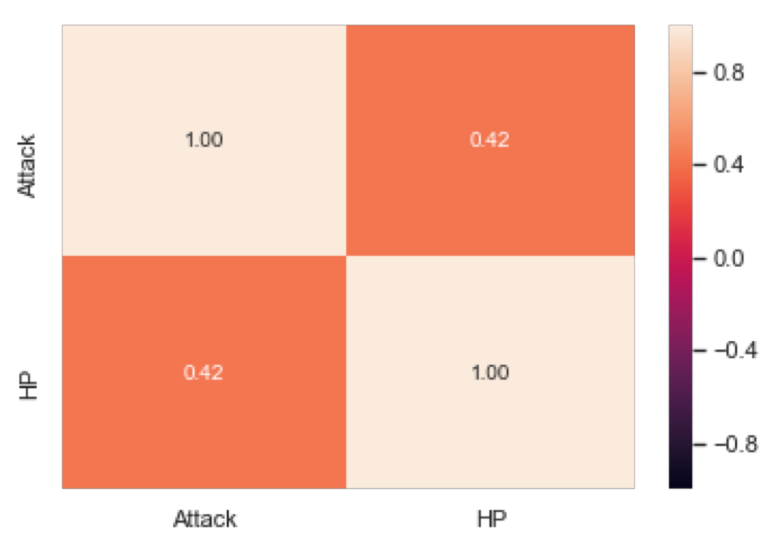
\includegraphics[width=.9\linewidth]{./images/2-variable-correlation-plot.png}
\end{center}
\subsubsection{Mutual correlation plot}
\label{sec:org8b6a829}
\begin{center}
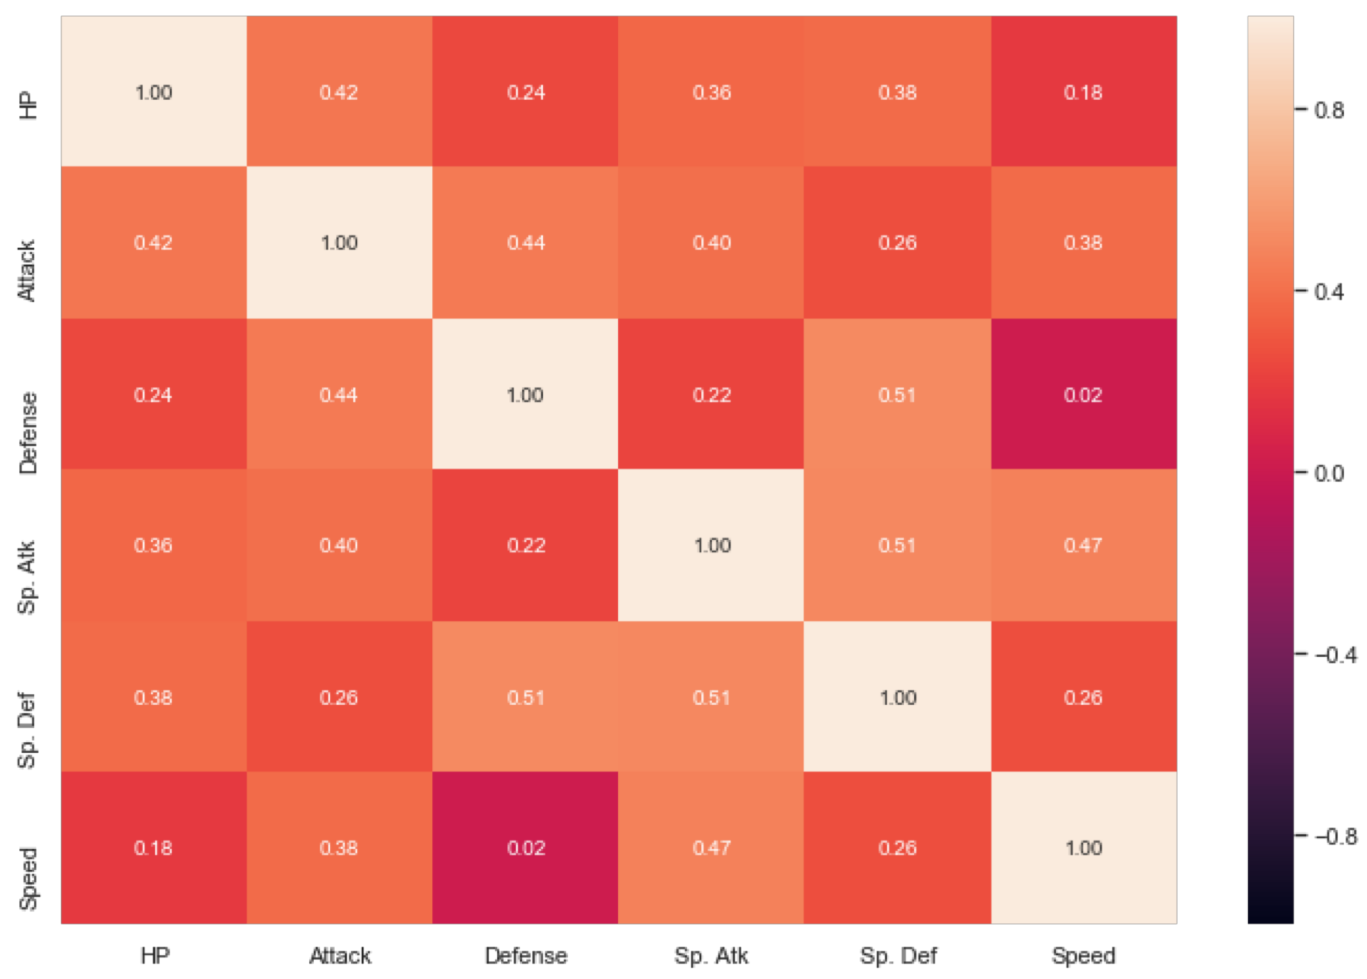
\includegraphics[width=.9\linewidth]{./images/mutual-correlation-plot.png}
\end{center}
\subsubsection{Examples}
\label{sec:orga508e02}
\begin{center}
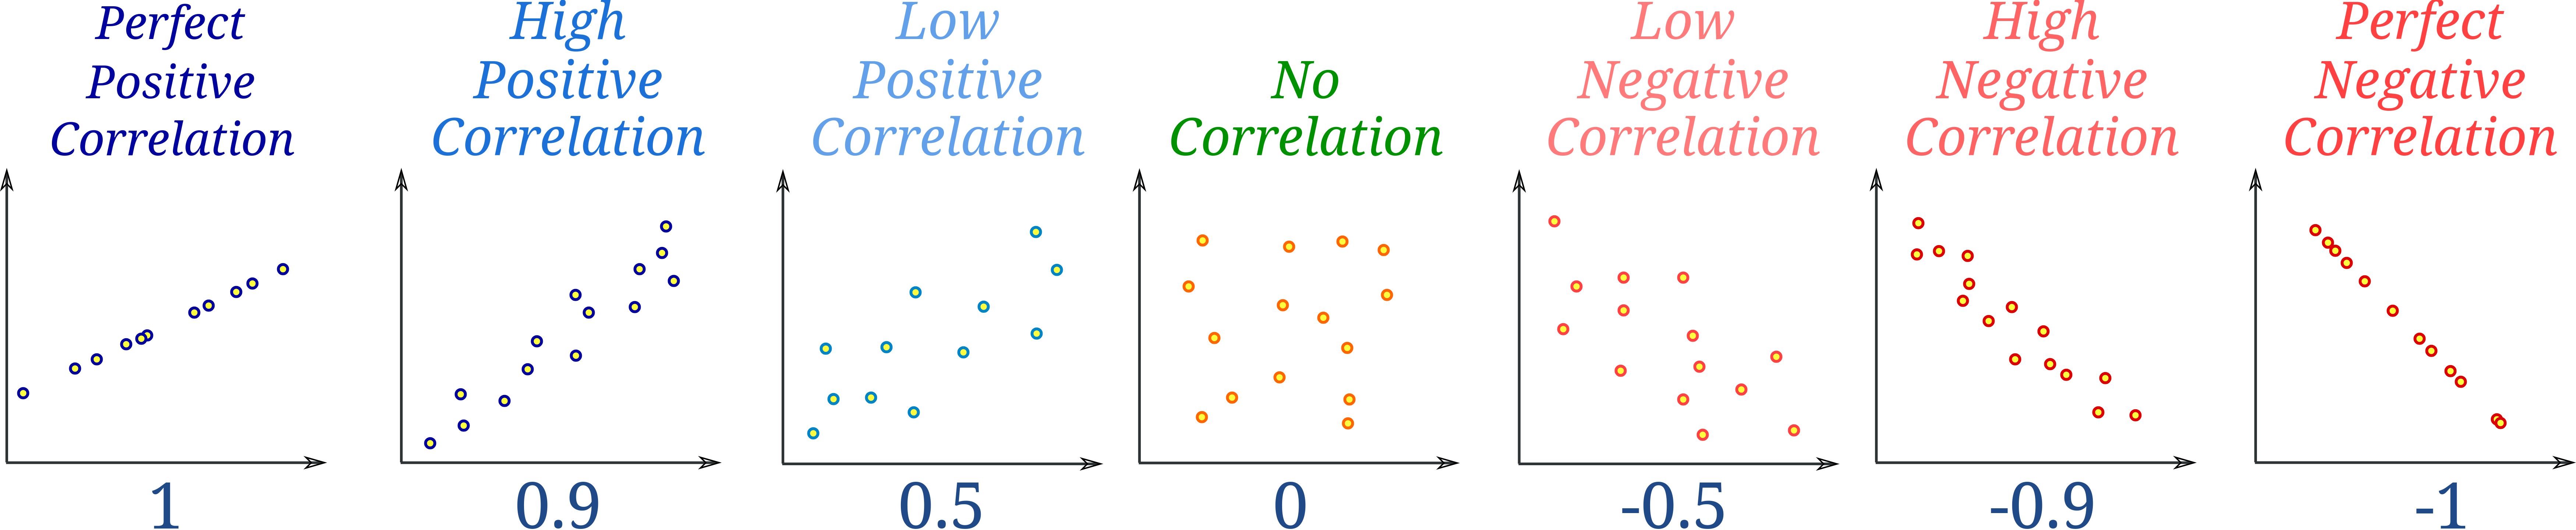
\includegraphics[width=.9\linewidth]{./images/correlation-examples.png}
\end{center}
\subsection{Residual sum of squares (\(RSS\))}
\label{sec:orgb3a0edb}
The residual sum of squares is defined as:
\[RSS = \sum (y_{actual} - y_{predicted})^2\]

Where:
\begin{itemize}
\item \(RSS\) is the residual sum of squares
\item \(y_{actual}\) is the actual value from the data set
\item \(y_{predicted}\) is the value predicted by the model
\end{itemize}
\subsection{Mean-squared error (\(MSE\))}
\label{sec:org2877d29}
The lower the mean-squared error (\(MSE\)), the better the model. Mean-squared error is defined as:
\[MSE = \frac{RSS}{n} \]

Where:
\begin{itemize}
\item \(MSE\) is the mean-squared error
\item \(RSS\) is the residual sum of squares
\item \(n\) is the number of items in the data set
\end{itemize}

 \newpage
\subsection{Total sum of squares (\(TSS\))}
\label{sec:org58aca54}
The total sum of squares is sum of the difference between a data point and the mean of the data set, squared. It is defined as:
\begin{align*}
TSS &= \sum_{i = 1}^n (x_i - \bar{x})^2 \\
&= (x_1 - \bar{x})^2 + (x_2 - \bar{x})^2 + \cdots + (x_n - \bar{x})^2
\end{align*}

Where:
\begin{itemize}
\item \(TSS\) is the total sum of squares
\item \(n\) is the total number of items in the data set
\item \(x\) is a data point
\item \(\bar{x}\) is the mean of the data set
\end{itemize}
\subsection{Variance (\(VAR\))}
\label{sec:org1ecd7a0}
The variance is the expected deviation from the mean, squared. It measures how far a set of numbers is spread from their average value. It is defined as:
\[VAR = \frac{TSS}{n}\]

Where:
\begin{itemize}
\item \(VAR\) is the variance
\item \(TSS\) is the total sum of squares
\item \(n\) is the number of items
\end{itemize}
\subsection{Explained variance (\(R^2\))}
\label{sec:org09e3cb3}
The higher the explained variance (\(R^2\)), the better the model. Explained variance is defined as:
\[R^2 = 1 - \frac{MSE}{VAR}\]

Where:
\begin{itemize}
\item \(R^2\) is the explained variance
\item \(MSE\) is the mean-squared error
\item \(VAR\) is the variance
\end{itemize}
\subsection{Gini Index (Gini Impurity)}
\label{sec:orgf96fc94}
The Gini Index tells you the chance of misclassification when you are in a specific partition of your data. It is defined as follows:
\begin{align*}
Gini &= \sum_{i = 1}^n \frac{x_i}{N} \left(1 - \frac{x_i}{N} \right) \\
&= \frac{x_1}{N} \left(1 - \frac{x_1}{N} \right) + \frac{x_2}{N} \left(1 - \frac{x_2}{N} \right) + \cdots + \frac{x_n}{N} \left(1 - \frac{x_n}{N} \right)
\end{align*}

Where:
\begin{itemize}
\item \(Gini\) is the Gini Index
\item \(x\) is the number of items belonging to a class in the data partition
\item \(N\) is the total number of items in your data set
\end{itemize}

A simpler equation for two items is shown below:
\[Gini = \frac{x}{N} \left(1 - \frac{x}{N} \right) + \frac{y}{N} \left(1 - \frac{y}{N} \right)\]

Where:
\begin{itemize}
\item \(Gini\) is the Gini Index
\item \(x\) is the number of items belonging to one class in that node or partition
\item \(N\) is the total number of items in the that node or partition
\item \(y\) is the number of items belonging to the other class in that node or partition
\end{itemize}
\subsection{Within-cluster sum of squares}
\label{sec:orgb876a5f}
The within-cluster sum of squares is calculated as follows:
\begin{itemize}
\item Take the point that represents the middle of the cluster as a reference point.
\item For each point \textbf{in} the cluster, calculate the distance between the point and the reference point (the point in the middle of the cluster) and square it.
\item Sum up the distances for all the points, and you have the within-cluster sum of squares.
\end{itemize}
\subsection{Classification accuracy}
\label{sec:orgae1895b}
The classification accuracy is the number of items classified correctly over the total number of items. It is defined as:
\[\text{Classification accuracy} = \frac{T_p + T_n}{n}\]

Where:
\begin{itemize}
\item \(T_p\) is the number of true positives
\item \(T_n\) is the number of true negatives
\item \(n\) is the total number of items
\end{itemize}
\subsection{Classification accuracy metrics}
\label{sec:org55280e3}
The easy way to remember these metrics is to remember that the equations are always divided by themselves plus the inverse of themselves.
\subsubsection{True positive rate (\(tpr\))}
\label{sec:org1aa8795}
\[tpr = \frac{T_p}{T_p + F_n}\]

Where:
\begin{itemize}
\item \(tpr\) is the true positive rate
\item \(T_p\) is the number of true positives
\item \(F_n\) is the number of false negatives
\end{itemize}
\subsubsection{True negative rate (\(tnr\))}
\label{sec:org00428f9}
\[tnr = \frac{T_n}{T_n + F_p}\]

Where:
\begin{itemize}
\item \(tnr\) is the true negative rate
\item \(T_n\) is the number of true negatives
\item \(F_p\) is the number of false positives
\end{itemize}
\subsubsection{False positive rate (\(fpr\))}
\label{sec:org74b075d}
\[fpr = \frac{F_p}{F_p + T_n}\]

Where:
\begin{itemize}
\item \(fpr\) is the false positive rate
\item \(F_p\) is the number of false positives
\item \(T_n\) is the number of true negatives
\end{itemize}
\subsubsection{False negative rate (\(fnr\))}
\label{sec:org3f336d2}
\[fnr = \frac{F_n}{F_n + T_p}\]

Where:
\begin{itemize}
\item \(fnr\) is the false positive rate
\item \(F_n\) is the number of false negatives
\item \(T_p\) is the number of true positives
\end{itemize}
\subsection{Precision}
\label{sec:org6574743}
Precision is defined as:
\[P = \frac{T_p}{T_p + F_p}\]

Where:
\begin{itemize}
\item \(P\) is the precision
\item \(T_p\) is the number of true positives
\item \(F_p\) is the number of false positives
\end{itemize}

 \newpage
\subsection{Recall}
\label{sec:org1a012f3}
Recall is defined as:
\[R = \frac{T_p}{T_p + F_n}\]

Where:
\begin{itemize}
\item \(R\) is the recall
\item \(T_p\) is the number of true positives
\item \(F_p\) is the number of false positives
\end{itemize}

 \newpage
\subsection{Normal distribution}
\label{sec:org8db950a}
\begin{center}
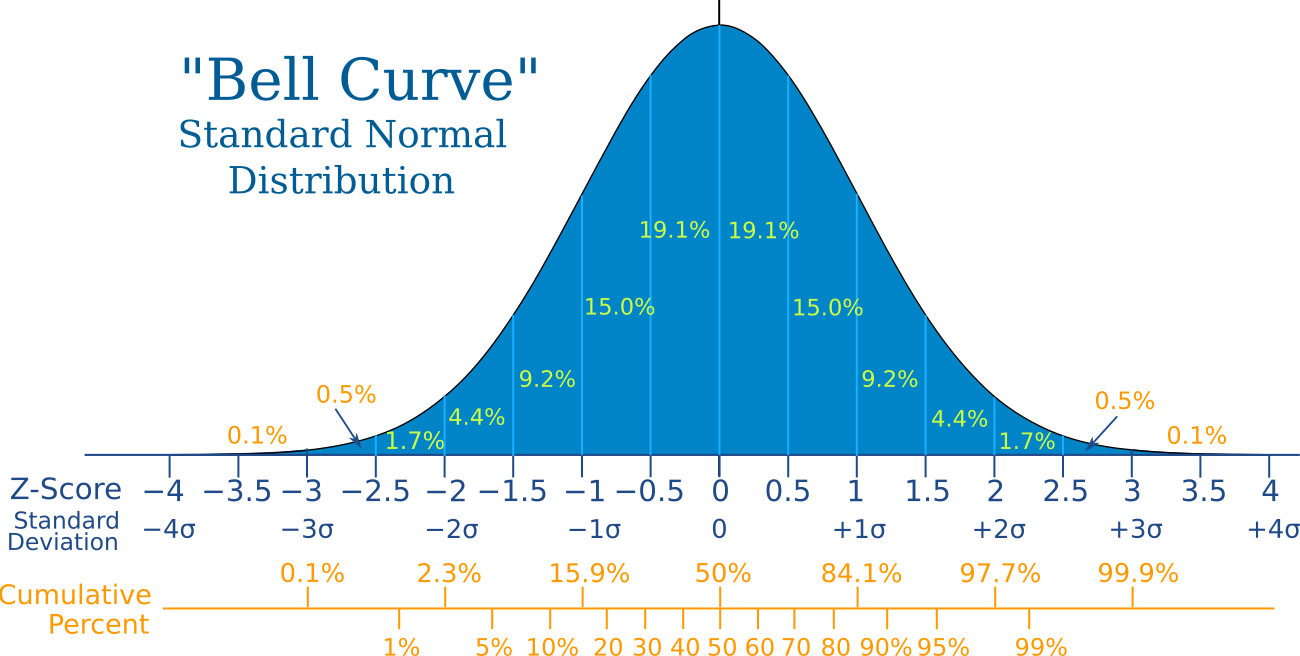
\includegraphics[width=.9\linewidth]{./images/normal-distribution-curve-granular-percentages.png}
\end{center}

\begin{center}
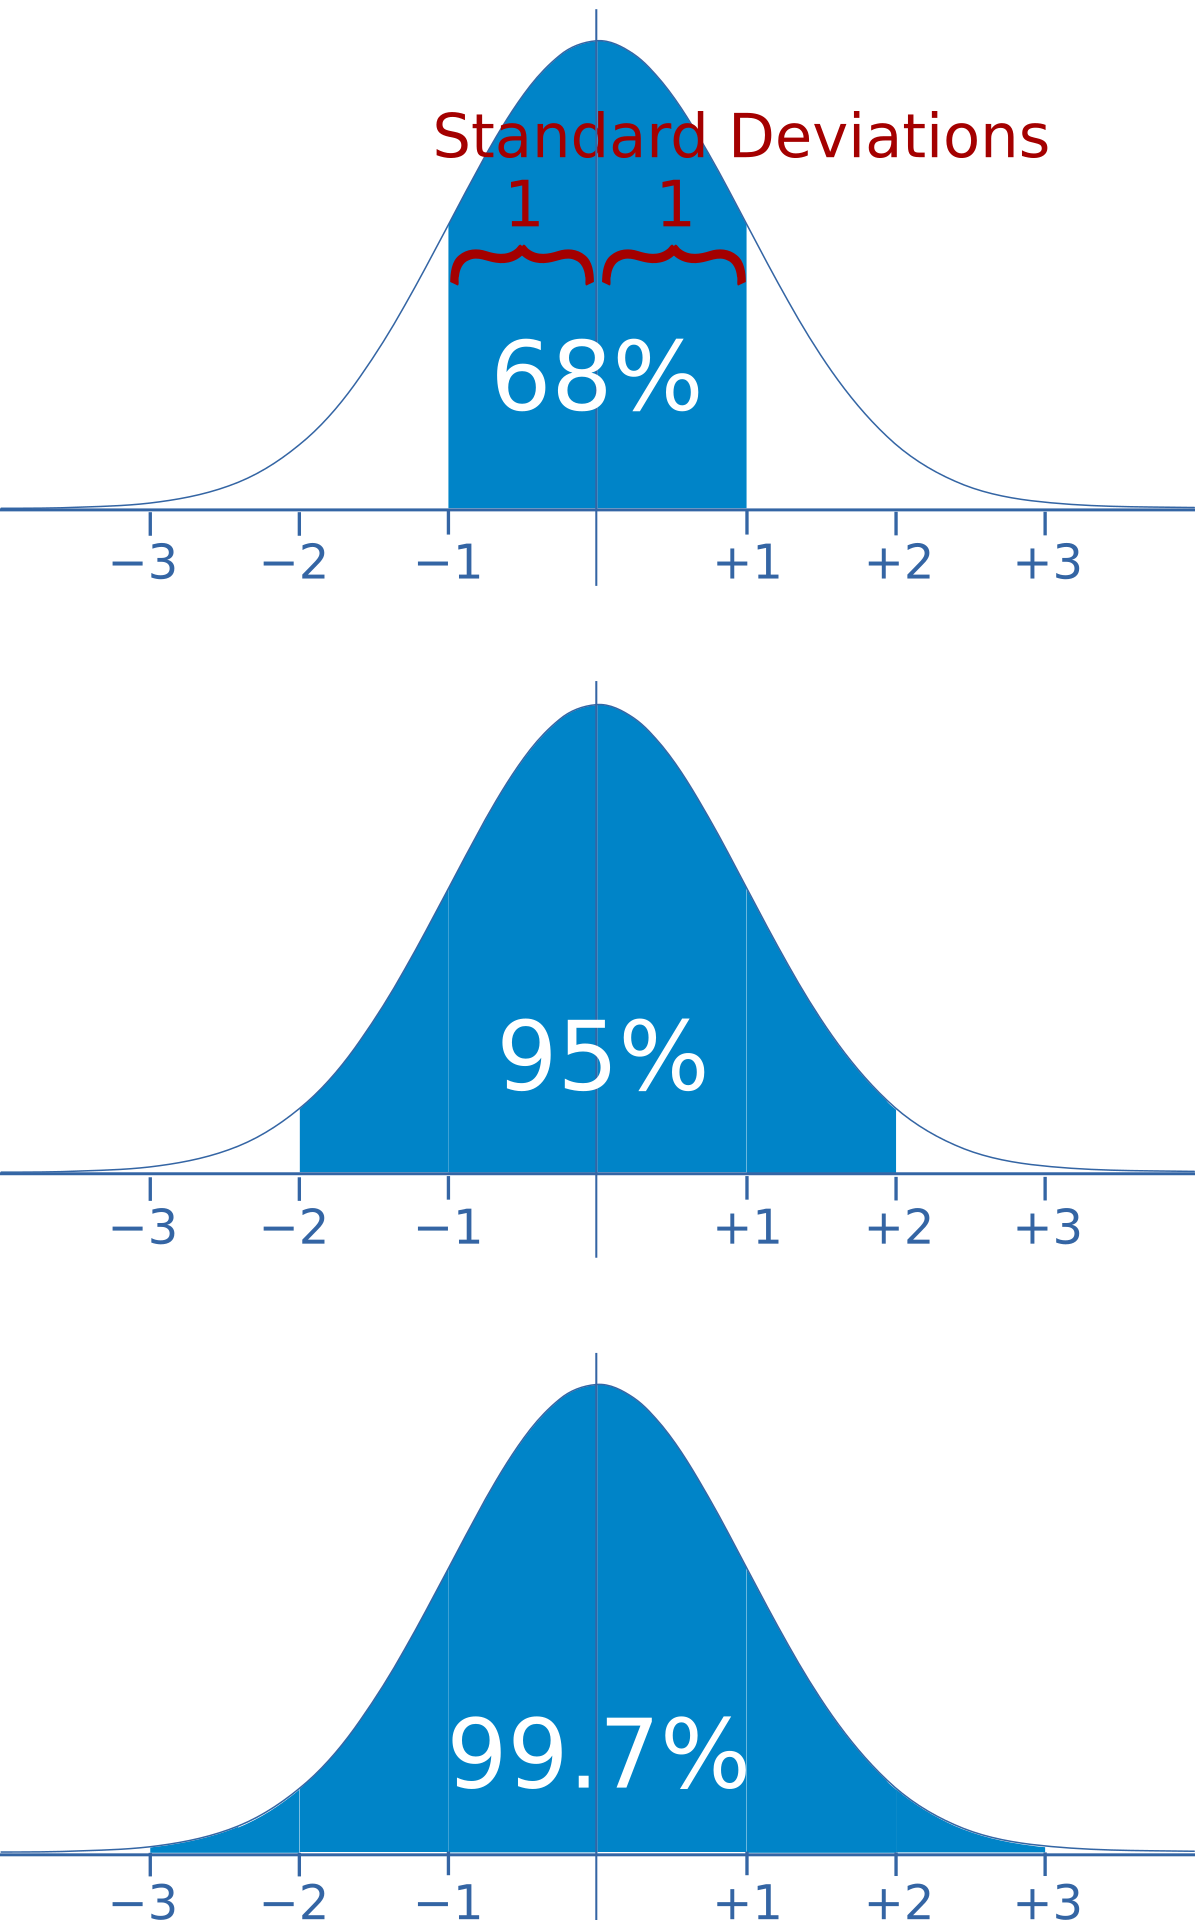
\includegraphics[height=32em]{./images/normal-distribution-curves-broad-percentages.png}
\end{center}
\subsection{Artificial Intelligence (AI)}
\label{sec:orgbb3cd1a}
AI is intelligence demonstrated by machines, in contrast to the *natural intelligence (NI) displayed by humans and other animals.
\subsection{Agent}
\label{sec:orgc0b5ed2}
An \textbf{agent} is an entity that \textbf{perceives} through sensors, like eyes, ears, cameras, and infrared range sensors, and \textbf{acts} through effectors, such as hands, legs and motors.

\begin{center}
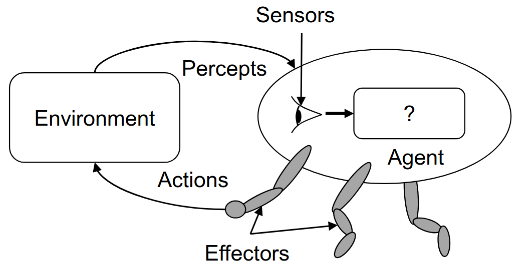
\includegraphics[width=.9\linewidth]{./images/agent-diagram.png}
\end{center}
\subsection{Rational action}
\label{sec:org46fe313}
A rational action is an action that maximises the expected value of an objective \textbf{performance} measure given the perception sequence to date.

 \newpage
\section{Data science pipeline}
\label{sec:orgd6aea0b}

\subsection{Practical motivation}
\label{sec:org649604e}
How to identify a data science case?
\begin{itemize}
\item What is the real-life problem?
\item Can you relate the problem to data?
\item Would data help you in practice?
\end{itemize}
\subsubsection{Sample collection}
\label{sec:orgb0503c9}
How to effectively sample real data?
\begin{itemize}
\item How to collect the relevant data?
\item Does the data match the problem?
\item Does the data represent reality?
\end{itemize}
\subsection{Problem formulation}
\label{sec:org74dc711}
How to intelligently construct a problem?
\begin{itemize}
\item What is the data science problem?
\item How do you formulate it using data?
\item How do you solve it using the data?
\end{itemize}
\subsubsection{Data preparation}
\label{sec:org6513711}
How to prepare raw data for analysis?
\begin{itemize}
\item How to prepare the relevant data?
\item Is the data clean enough to analyse?
\item Is the data structured for analysis?
\end{itemize}
\subsection{Statistical description}
\label{sec:org47e993c}
How to succinctly represent the data?
\begin{itemize}
\item How to clearly describe the data?
\item How do you summarise the data?
\item Which vital statistics are relevant?
\end{itemize}
\subsubsection{Exploratory analysis}
\label{sec:org95b6e42}
How to gain basic insight from data?
\begin{itemize}
\item How to explore the acquired data?
\item How to effectively mine the data?
\item How to compute the vital statistics?
\end{itemize}

How to intelligently explore acquired data?
\begin{itemize}
\item What are the variables in the data?
\item How to characterise the variables?
\item How to find relations between them?
\end{itemize}
\subsection{Pattern recognition}
\label{sec:orgd44b931}
How to find intrinsic insight from the data?
\begin{itemize}
\item How to identify structure in data?
\item Can you see the known patterns?
\item Can you discover unknown traits?
\end{itemize}
\subsubsection{Analytic visualisation}
\label{sec:org5100345}
How to represent the data for humans?
\begin{itemize}
\item How to clearly visualise the data?
\item How to visually represent statistics?
\item How to highlight "interesting" traits?
\end{itemize}
\subsection{Machine learning}
\label{sec:orge8e960b}
How to efficiently learn from the data?
\begin{itemize}
\item How to learn from the data?
\item Can you formulate the "learning"?
\item Can you automate the "learning"?
\end{itemize}
\subsubsection{Algorithmic optimisation}
\label{sec:orgf8effd1}
How to optimally learn from the data?
\begin{itemize}
\item How to form "learning" algorithms?
\item How to reduce errors in learning?
\item How to generalise the algorithms?
\end{itemize}
\subsection{Statistical inference}
\label{sec:org6c88008}
How to confidently infer from the data?
\begin{itemize}
\item How to draw conclusion from data?
\item Can you generalise the "learning"?
\item Can you estimate the confidence?
\end{itemize}
\subsubsection{Information presentation}
\label{sec:orgab00cfb}
How to communicate your data analysis?
\begin{itemize}
\item How to present analysis outcomes?
\item How to present descriptive analysis?
\item How to present inferential analysis?
\end{itemize}
\subsection{Intelligent decision}
\label{sec:orgbde3984}
How to solve a real-life problem by data?
\begin{itemize}
\item How to make decisions in practice?
\item Can you decide based on the data?
\item Can you optimise the outcomes?
\end{itemize}
\subsubsection{Ethical consideration}
\label{sec:orgdb1311c}
How to responsibly work in data science?
\begin{itemize}
\item How to conform to ethical values?
\item Does the analysis violate legality?
\item Does the decision violate ethics?
\end{itemize}

 \newpage
\section{Data science problems and solutions}
\label{sec:org08dcadb}

\subsection{How much? How many?}
\label{sec:org20fed12}
The model should \textbf{predict} a \textbf{numeric} value.

Examples:
\begin{itemize}
\item What is the expected sales of the next game of this game franchise?
\item Is it profitable to make the sequel?
\end{itemize}
\subsubsection{Solution: Regression}
\label{sec:org58bbfa4}
Try to find the relationship of sales of the games with other variables, like graphics quality, genre, etc.

\[\text{Model: } \text{Sales} = f(\text{Variables})\]

Examples:
\begin{itemize}
\item Linear regression models
\item Tree models for regression
\item Neural network for regression
\end{itemize}
\subsection{Is it type A or type B?}
\label{sec:orgd29f018}
The model should \textbf{predict} a \textbf{category} or a \textbf{class} for an object.

Examples:
\begin{itemize}
\item What is the chance that a student will get into NTU in AY2019-2020?
\item Will an application be successful?
\end{itemize}
\subsubsection{Solution: Classification}
\label{sec:org1564ed6}
Try to find the probability of getting admitted to NTU in terms of other variables, like scores, gender, etc.

\[\text{Model: } \mathcal{P} (\text{Admit}) = f(\text{Variables})\]

Examples:
\begin{itemize}
\item Logistic Regression Model
\item Tree models for classification
\item Neural network for classification
\end{itemize}
\subsection{How is this organised?}
\label{sec:org566e946}
The model should \textbf{detect} the \textbf{structure} of an object.

Examples:
\begin{itemize}
\item Is there any structure apparent within the FairPrice customers?
\item Which customer group to target?
\end{itemize}
\subsubsection{Solution: Clustering}
\label{sec:orgcf6c580}
Try to find groups of data points that are close together but far from the other groups of points. How close and how far depends on the "distance", like the Minkowski distance, as shown below:

\[D(X, Y) = \left(\sum_{i = 1}^n \left| x_i - y_i \right|^p \right)^{\frac{1}{p}}\]

Some examples of "distances":
\begin{itemize}
\item Euclidean distance
\item Jaccard distance
\end{itemize}

Examples of clustering models:
\begin{itemize}
\item k-Means algorithm for clustering
\item Hierarchical model for clustering
\end{itemize}
\subsection{Is it weird behaviour?}
\label{sec:org1e6612a}
The model should \textbf{detect anomalies} in the data.

Examples:
\begin{itemize}
\item Is this Boeing engine behaving unusually during the flight?
\item Is the engine still safe to operate?
\end{itemize}
\subsubsection{Solution: Anomaly detection}
\label{sec:orgc2f5a59}
Try to find deviations in the data compared to the regular pattern observed through the data model. The deviations depend on the model.

Examples:
\begin{itemize}
\item Cluster-analysis based detection
\item Nearest neighbour detection model
\item Support vector-based detection
\end{itemize}
\subsection{What should be done next?}
\label{sec:org7fad579}
The model should \textbf{detect} the next \textbf{action} to be done.

Examples:
\begin{itemize}
\item Should the car brake at the yellow light, or should the car accelerate instead?
\item Which action will be rewarded?
\end{itemize}
\subsubsection{Solution: Adaptive learning}
\label{sec:orga79ef12}
Try to model a profit or loss function depending on the given state, and try to maximise the profit or minimise the loss, respectively.

\[\text{Optimisation function}: f(\text{State, Variables})\]

Examples of using the reinforcement learning approach:
\begin{itemize}
\item Monte-Carlo
\item State-Action-Reward
\item Q-Learning
\item Deep Reinforcement
\end{itemize}

 \newpage
\section{Common data types}
\label{sec:org6d5c150}

\subsection{Structured data}
\label{sec:orgebfc0e9}
\begin{itemize}
\item Highly organised
\item Easy to analyse
\end{itemize}
\subsubsection{Numeric data}
\label{sec:orgc37b80e}
\begin{itemize}
\item Highly organised data
\item Clearly defined variables
\item Easy to mine and analyse
\item Numeric continuous variables
\end{itemize}

Possible sources:
\begin{itemize}
\item Spreadsheets (Excel, CSV)
\item Standard SQL databases
\item Sensors and devices
\end{itemize}
\subsubsection{Categorical data}
\label{sec:org14439c5}
\begin{itemize}
\item Highly organised data
\item Clearly defined variables
\item Easy to mine and analyse
\item Factor, level or class variables
\end{itemize}

Possible sources:
\begin{itemize}
\item Spreadsheets (Excel, CSV)
\item Standard SQL databases
\item Sensors and devices
\end{itemize}
\subsubsection{Mixed data}
\label{sec:org80fbc76}
\begin{itemize}
\item Highly organised data
\item Clearly defined variables
\item Easy to mine and analyse
\item Numeric and categorical
\end{itemize}

Possible sources:
\begin{itemize}
\item Spreadsheets (Excel, CSV)
\item Standard SQL databases
\item Sensors and devices
\end{itemize}
\subsubsection{Time series data}
\label{sec:org3f39f15}
\begin{itemize}
\item Highly organised data
\item Clearly defined variables
\item Easy to mine and analyse
\item Numeric with timestamps
\end{itemize}

Possible sources:
\begin{itemize}
\item Stock and equity markets
\item Weather data over time
\item Prices and promotions
\end{itemize}

 \newpage
\subsubsection{Network data}
\label{sec:org40fa7df}
\begin{itemize}
\item Highly organised data
\item Clearly defined variables
\item Easy to mine and analyse
\item Numeric with timestamps
\end{itemize}

Possible sources:
\begin{itemize}
\item Social networks and the web
\item Transport networks (MRT)
\item Financial transactions
\end{itemize}
\subsection{Unstructured data}
\label{sec:orgac0c685}
\begin{itemize}
\item Highly unorganised
\item Contextual
\end{itemize}
\subsubsection{Text data}
\label{sec:org139bdf5}
\begin{itemize}
\item Highly unorganised data
\item Non-obvious variables
\item Highly context-sensitive
\item Words, phrases and emoticons
\end{itemize}

Possible sources:
\begin{itemize}
\item Social networks and the web
\item Text messages or WhatsApp
\item Books, wikis and documents
\end{itemize}
\subsubsection{Image data}
\label{sec:orge7e40be}
\begin{itemize}
\item Highly unorganised data
\item Non-obvious variables
\item Highly context-sensitive
\item Words, phrases and emoticons
\end{itemize}

Possible sources:
\begin{itemize}
\item Social networks and the web
\item Mobile phone cameras
\item Blogs, wikis and documents
\end{itemize}
\subsubsection{Video data}
\label{sec:org89f1720}
\begin{itemize}
\item Highly unorganised data
\item Non-obvious variables
\item Highly context-sensitive
\item Images, frames and objects
\end{itemize}

Possible sources:
\begin{itemize}
\item YouTube and social media
\item Video messages and calls
\item Mobile phone cameras
\end{itemize}

 \newpage
\subsubsection{Voice data}
\label{sec:orgcf1520d}
\begin{itemize}
\item Highly unorganised data
\item Non-obvious variables
\item Highly context-sensitive
\item Voice signals and waves
\end{itemize}

Possible sources:
\begin{itemize}
\item Songs and social media
\item Microphones and cameras
\item Recordings and announcements
\end{itemize}
\section{Plots}
\label{sec:org3e262b5}

\subsection{Uni-variate box-plot}
\label{sec:org1eb338c}
\begin{center}
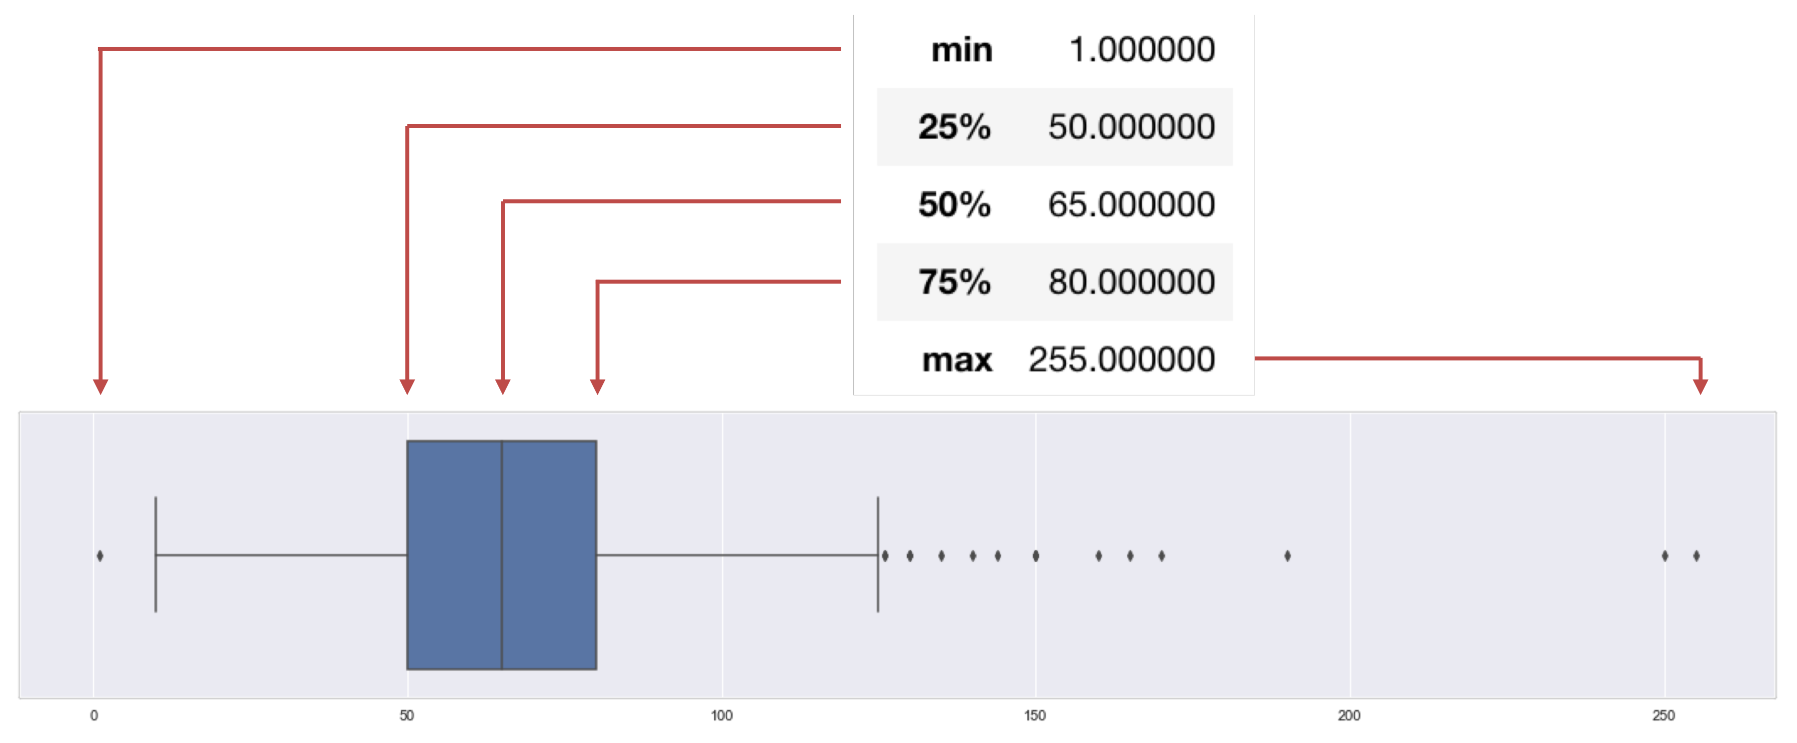
\includegraphics[width=.9\linewidth]{./images/uni-variate-box-plot.png}
\end{center}
\subsection{Uni-variate histogram}
\label{sec:orgf49b1c5}

\subsubsection{Variation 1}
\label{sec:orge9222a0}
\begin{center}
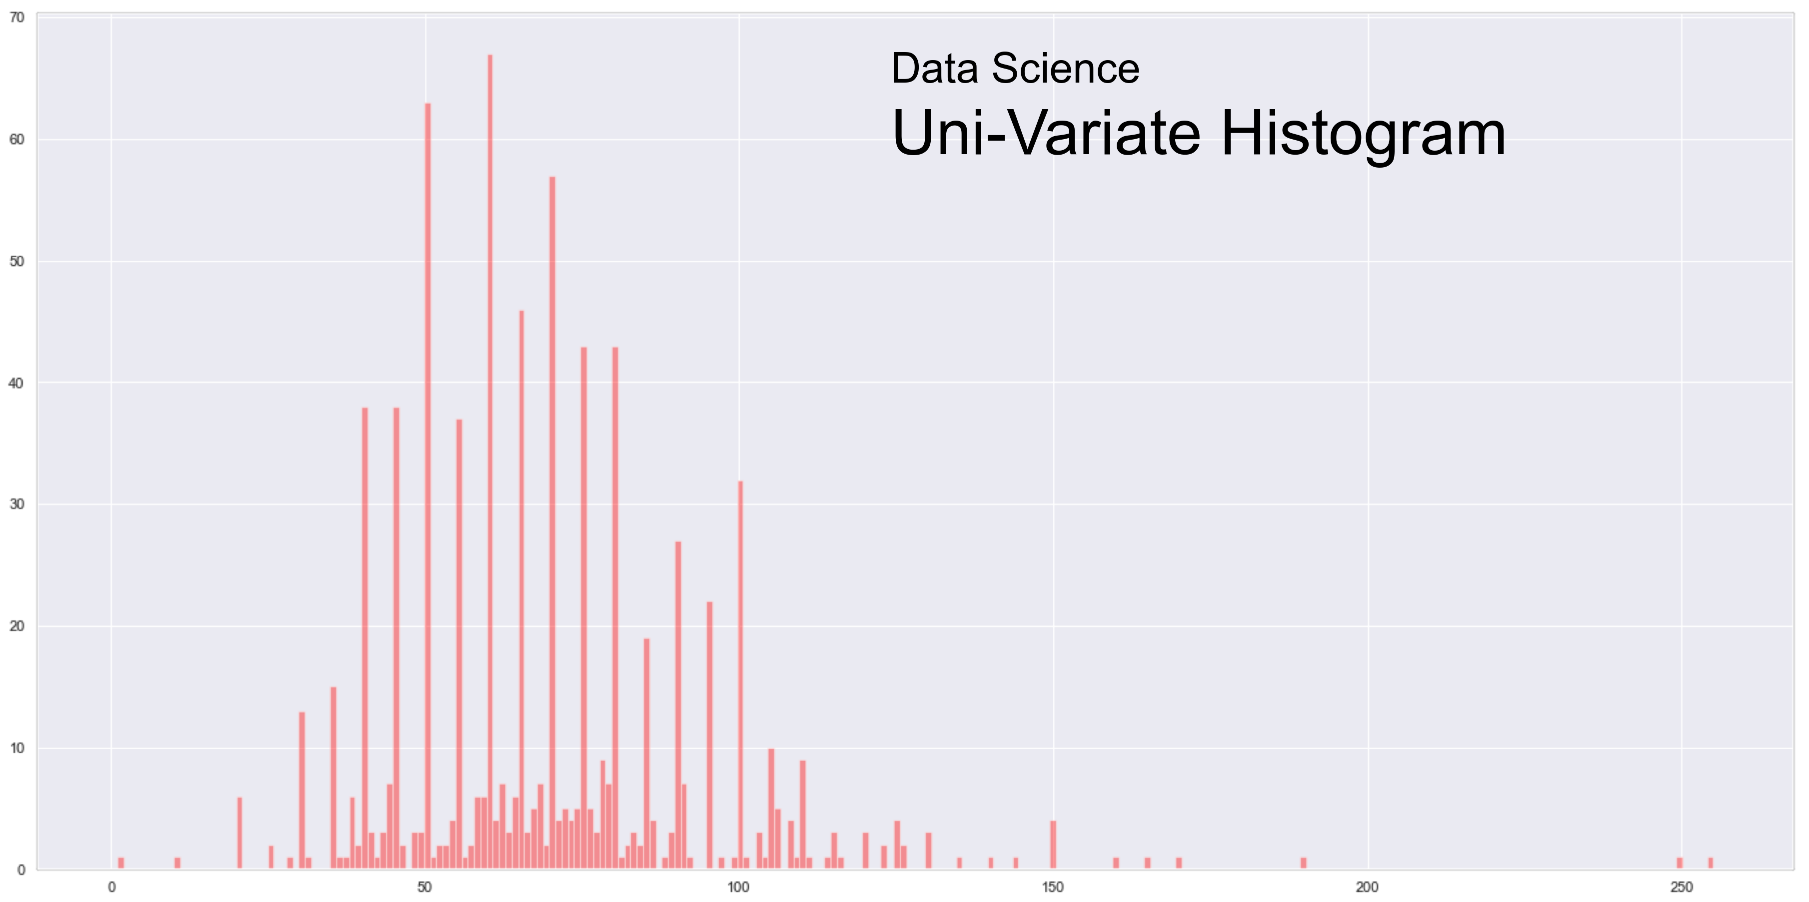
\includegraphics[width=.9\linewidth]{./images/uni-variate-histogram-variation-1.png}
\end{center}
\subsubsection{Variation 2}
\label{sec:org2ec3975}
\begin{center}
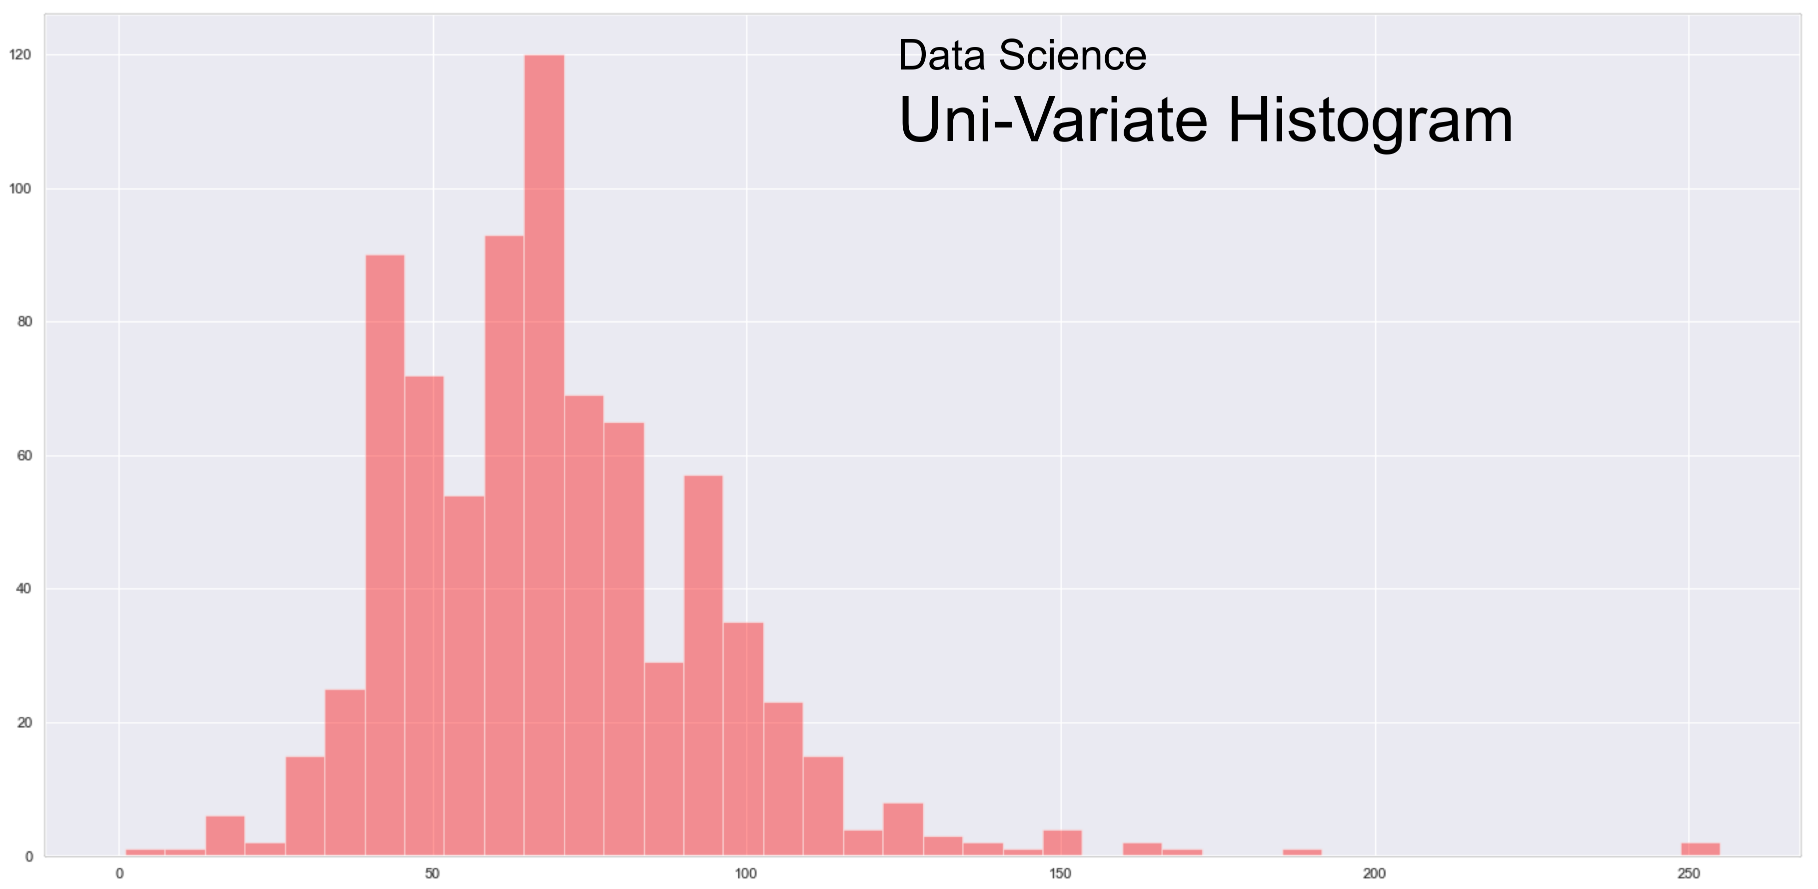
\includegraphics[width=.9\linewidth]{./images/uni-variate-histogram-variation-2.png}
\end{center}
\subsection{Uni-variate density plot}
\label{sec:orgce45b1a}
\begin{center}
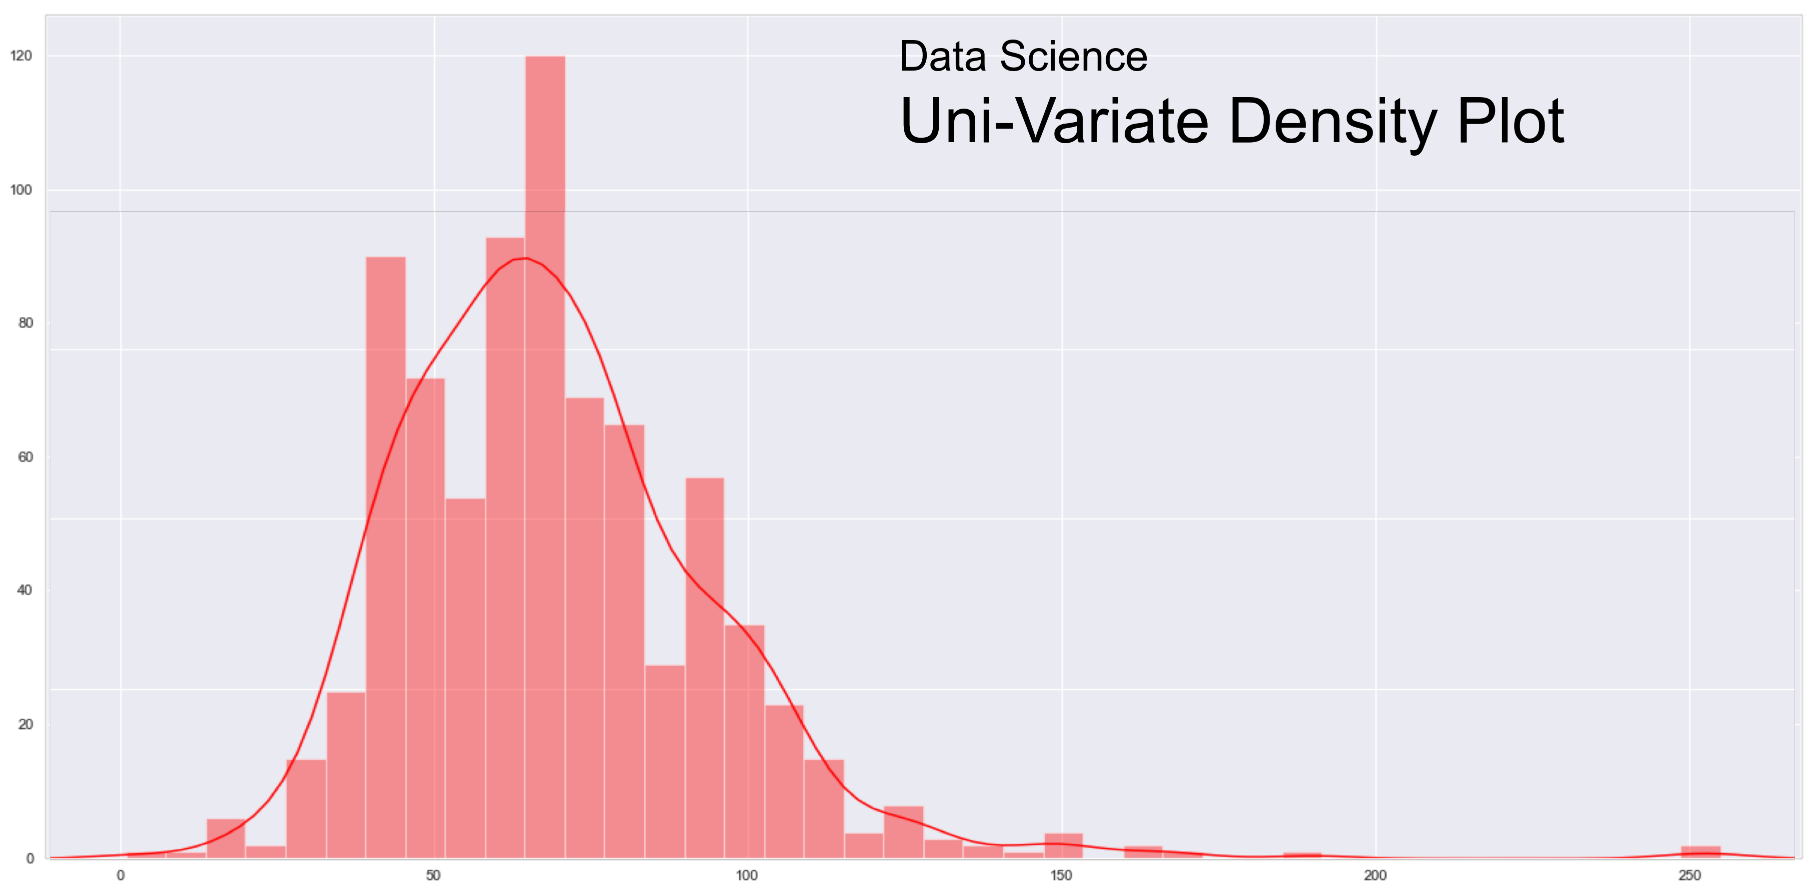
\includegraphics[width=.9\linewidth]{./images/uni-variate-density-plot.png}
\end{center}
\subsection{Uni-variate violin plot}
\label{sec:org18eee74}
\begin{center}
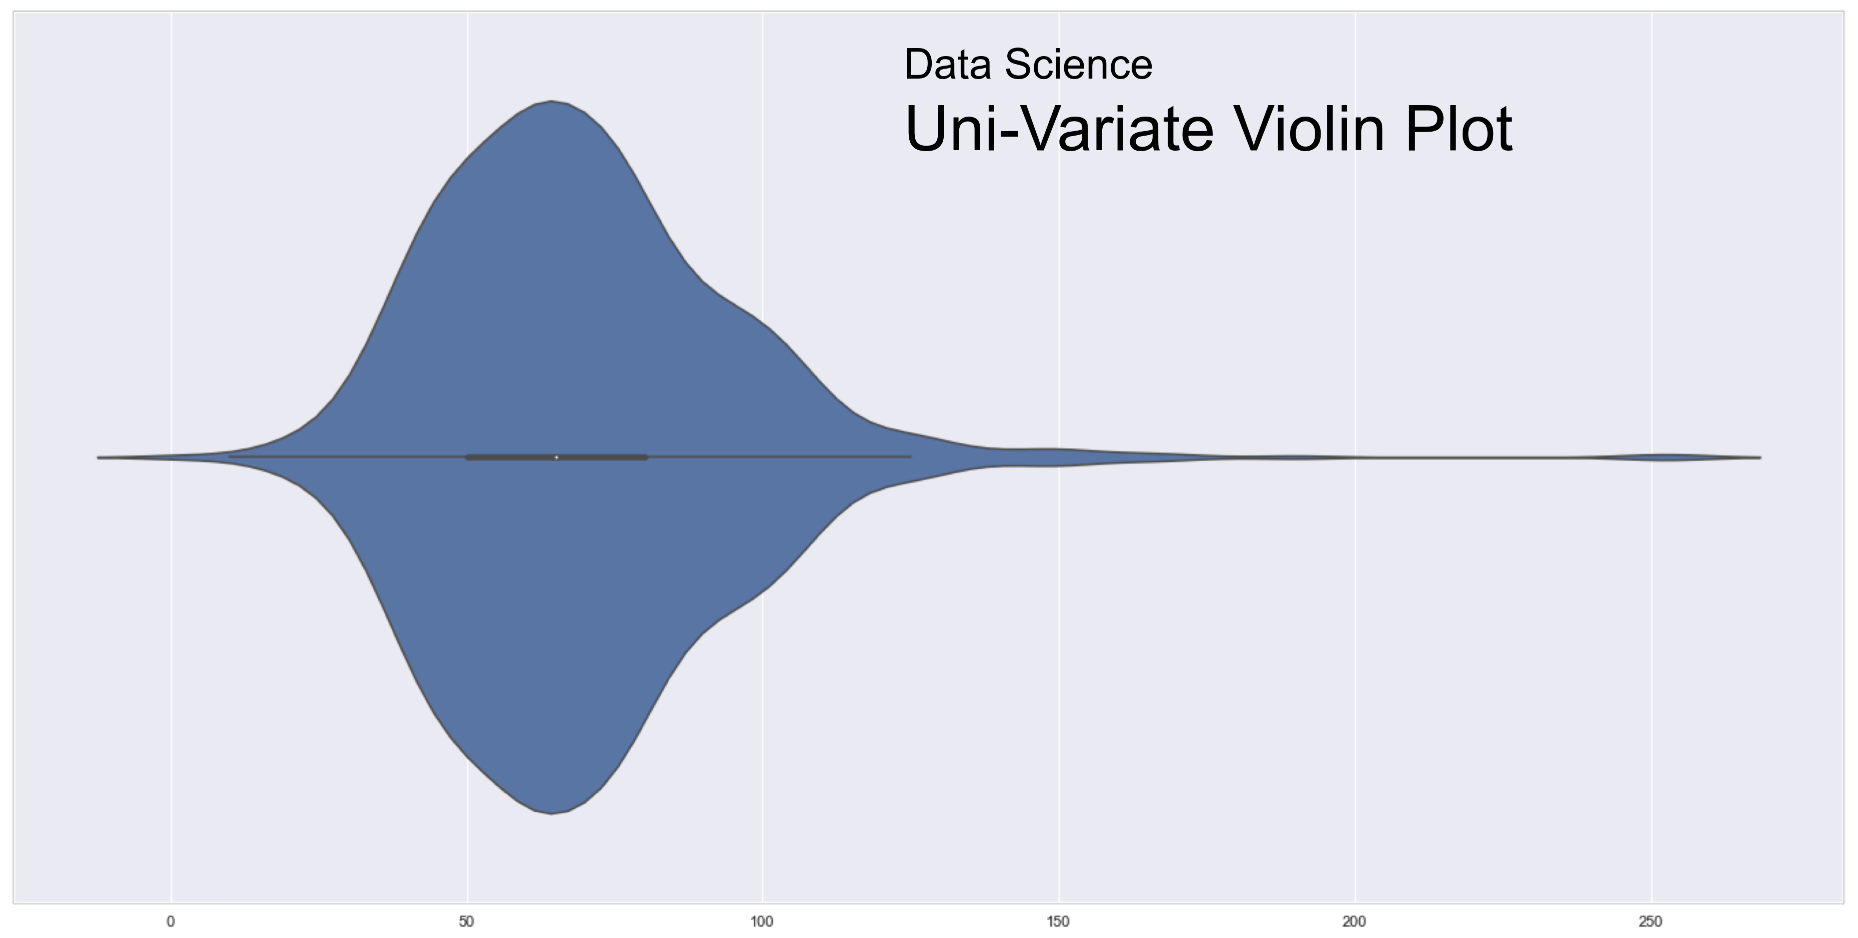
\includegraphics[width=.9\linewidth]{./images/uni-variate-violin-plot.png}
\end{center}
\subsection{Uni-variate swarm-plot}
\label{sec:orgf126e4a}
\begin{center}
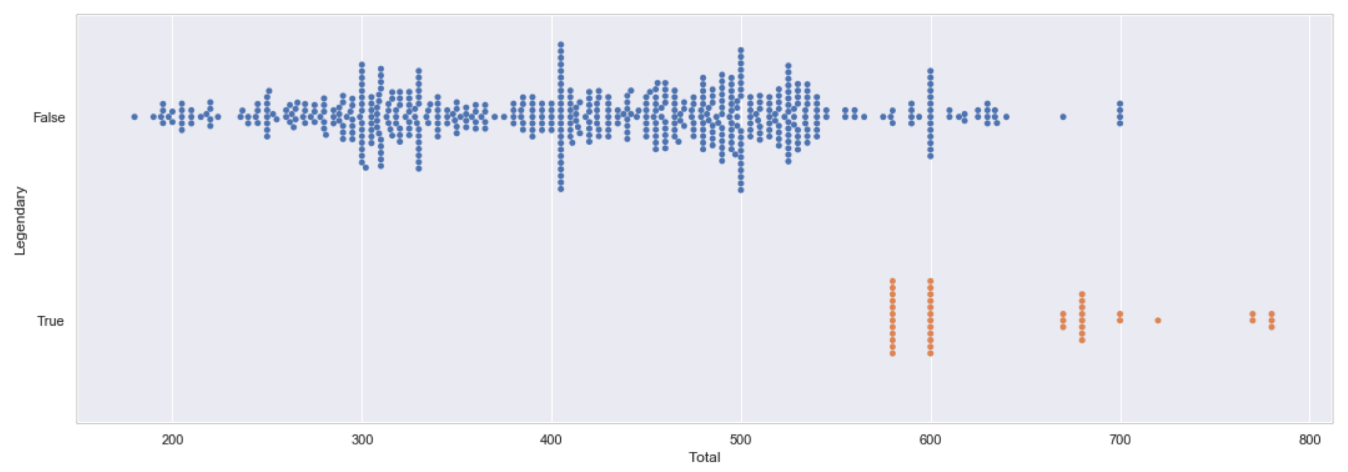
\includegraphics[width=.9\linewidth]{./images/uni-variate-swarm-plot.png}
\end{center}
\subsection{Bivariate joint plot}
\label{sec:org16ee4ca}
\begin{center}
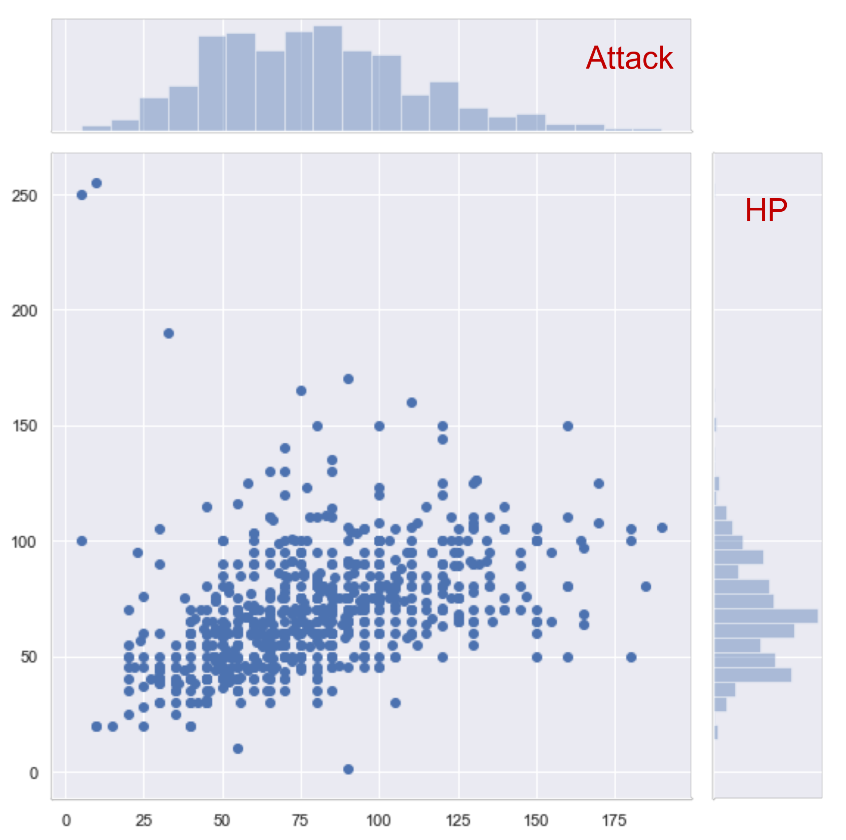
\includegraphics[width=.9\linewidth]{./images/bi-variate-joint-plot.png}
\end{center}

 \newpage
\section{Machine learning}
\label{sec:org2d1d16a}
How to optimally learn from the data?
\begin{itemize}
\item What do we know about the problem?
\item Does the data provide hints?
\item Can we learn from the hints in the data?
\item Can we test how well we have learnt?
\end{itemize}
\subsection{Supervised learning}
\label{sec:org13228e9}
\begin{itemize}
\item Regression
\item Classification
\end{itemize}
\subsection{Unsupervised learning}
\label{sec:orgd45b5c4}
\begin{itemize}
\item Clustering
\item Anomaly detection
\end{itemize}
\subsection{Numeric prediction problem}
\label{sec:org8a4ea0e}
\begin{itemize}
\item How much?
\item How many?
\end{itemize}
\subsubsection{Regression}
\label{sec:orge2df95e}
\[\text{Model: Total} = f(\text{Variables}) \]

For example:
\begin{itemize}
\item Given some Pokémon to train.
\item Learn the model for total points.
\item Predict the estimated total for the others.
\end{itemize}
\subsection{Classes prediction problem}
\label{sec:orgaf146d5}
Is it type A or type B?
\subsubsection{Classification}
\label{sec:org0bee356}
\[\text{Model: } P (\text{Legend}) = f(\text{Variables})\]

For example:
\begin{itemize}
\item Given some Pokémon to train.
\item Learn the model for legendary Pokémon.
\item Determine the class for others.
\end{itemize}
\subsection{Structure detection problem}
\label{sec:orgd88882b}
How is this organised?
\subsubsection{Clustering}
\label{sec:orgf167c23}
Grouping depends on "distance".

For example:
\begin{itemize}
\item Given the distance on all Pokémon.
\item Find the optimal groups in the data.
\item Justify the interpretation of the groups.
\end{itemize}
\subsection{Anomaly detection problem}
\label{sec:org6ed3592}
Is it weird behaviour?

 \newpage
\section{Uni-variate regression}
\label{sec:orgd2431e4}
\begin{itemize}
\item Are variables mutually dependent?
\item How to find the relations between them?
\item How to predict one using the other?
\end{itemize}
\subsection{Split the data set into 2}
\label{sec:org352264f}
\begin{enumerate}
\item A training data set to train the model.
\item A testing data set to test the model's performance.
\end{enumerate}

The objectives:
\begin{itemize}
\item Learn the relationship from the training data set.
\item Try to predict the total on the testing data set.
\end{itemize}
\subsection{Statistical modelling}
\label{sec:org2b55e3f}

\subsubsection{Hypothesise a linear model}
\label{sec:org3967752}
\[y = ax + b\]

Where:
\begin{itemize}
\item \(y\) is the dependent variable, like the ranking of Pokémon, for example
\item \(a\) is a constant that we need to find
\item \(x\) is the independent variable, like the HP of a Pokémon, for example
\item \(b\) is another constant that we need to find
\end{itemize}
\subsubsection{Steps}
\label{sec:org2e0512d}
\begin{enumerate}
\item Guess parameters \(a\) and \(b\) in the model.
\item Predict the values of the \textbf{dependent variable}, \(y\), in the training data.
\item Calculate the \textbf{errors} in the predicted value compared to the actual data.
\item Tune the parameters \(a\) and \(b\) to minimise errors.
\end{enumerate}
\subsubsection{Algorithmic optimisation}
\label{sec:org3b005b4}
The cost function to minimise errors is the total-squared error:
\[J(a, b) = \sum(y - ax - b)^2\]
\subsubsection{Learning from training data}
\label{sec:org1ddfe96}
\begin{center}
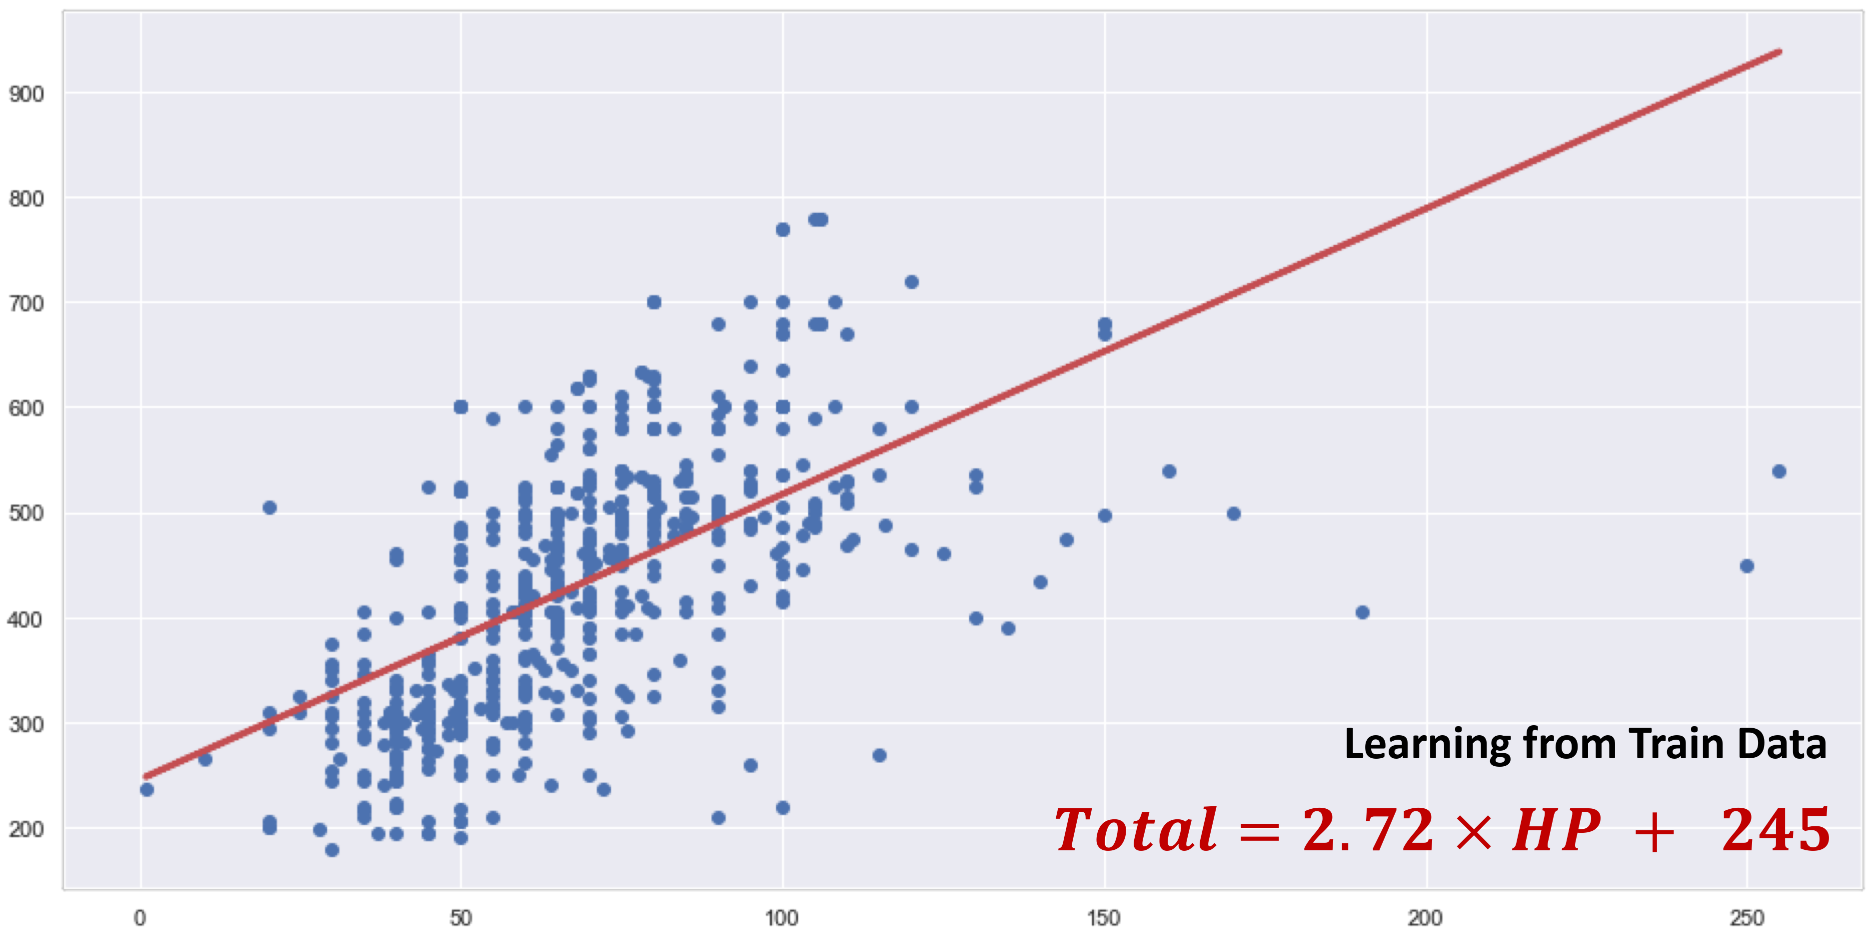
\includegraphics[width=.9\linewidth]{./images/learning-from-training-data.png}
\end{center}
\subsubsection{Prediction on test data}
\label{sec:org6cc6d0e}
\begin{center}
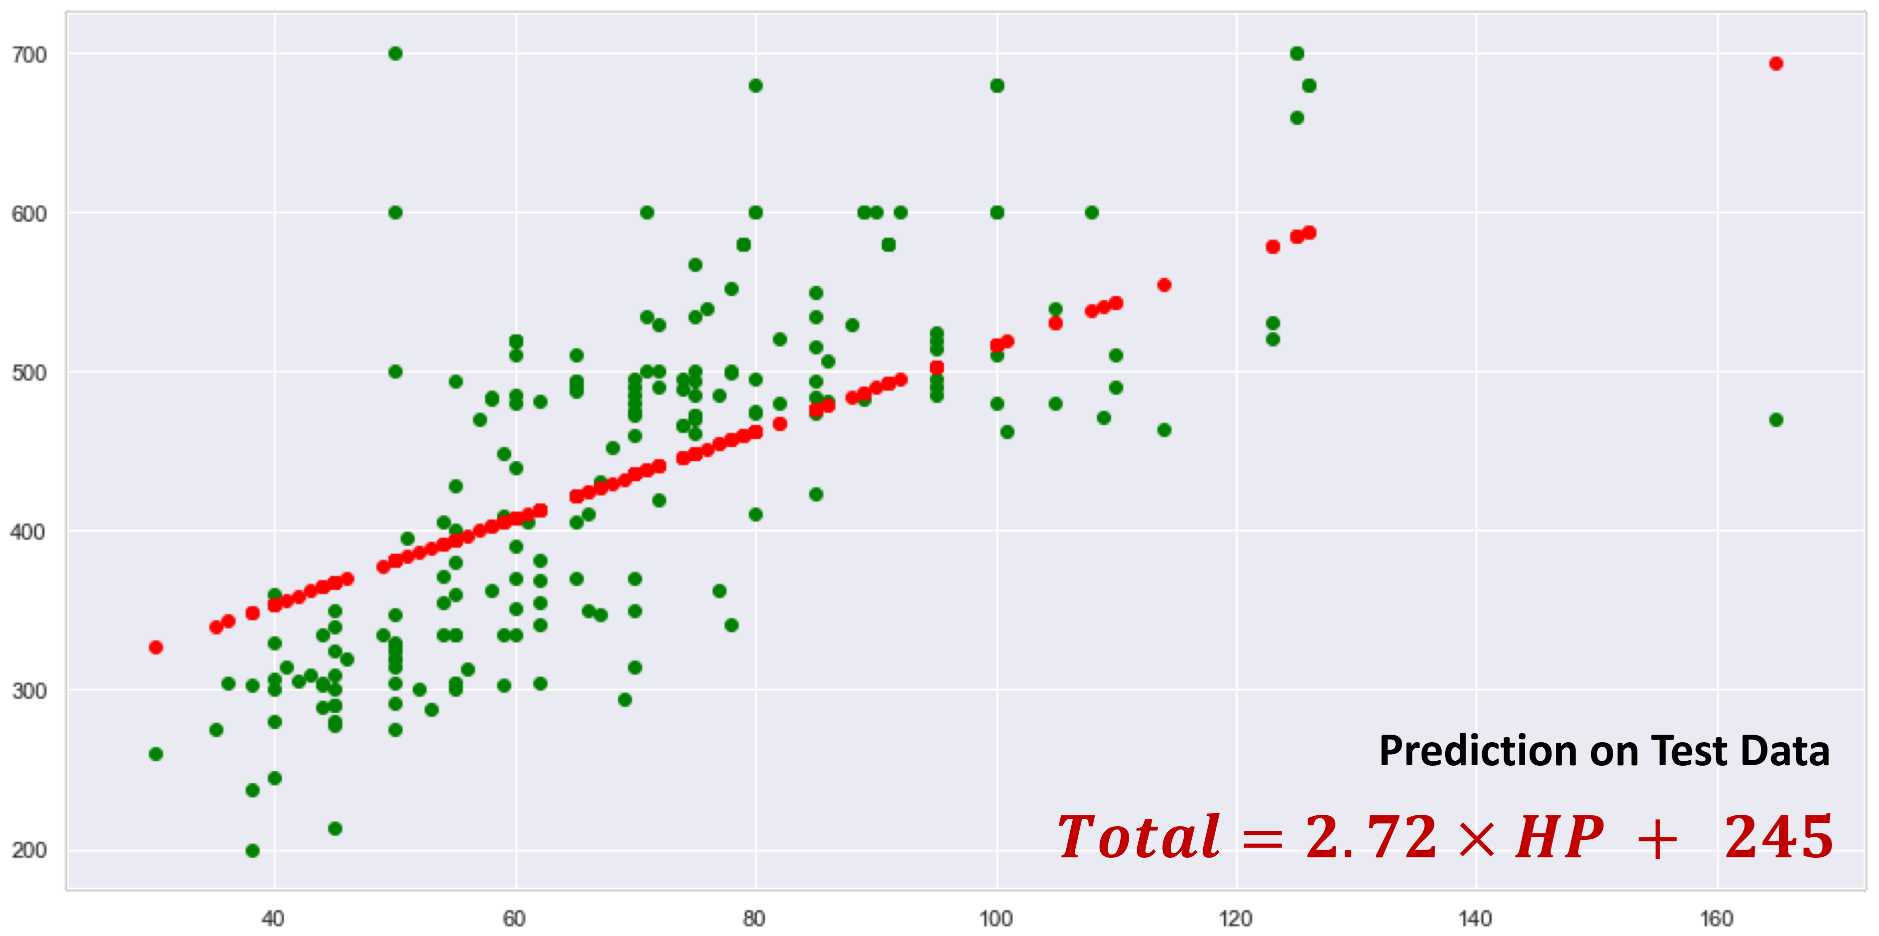
\includegraphics[width=.9\linewidth]{./images/prediction-on-test-data.png}
\end{center}

 \newpage
\subsection{Performance evaluation}
\label{sec:org21ff230}
The hypothesised model is a linear model:
\[y = ax + b\]

Where:
\begin{itemize}
\item \(y\) is the dependent variable, like the ranking of Pokémon, for example
\item \(a\) is a constant that we need to find
\item \(x\) is the independent variable, like the HP of a Pokémon, for example
\item \(b\) is another constant that we need to find
\end{itemize}
\subsubsection{Mean-squared error (\(MSE\))}
\label{sec:org0fcc3b5}
The lower the mean-squared error (\(MSE\)), the better the model. Mean-squared error is defined as:
\[MSE = \frac{1}{n} \sum (y - ax - b)^2\]

Where:
\begin{itemize}
\item \(MSE\) is the mean-squared error
\item \(n\) is the number of items in the data set
\item \(y\) is the dependent variable, like the ranking of Pokémon, for example
\item \(a\) is a constant that we need to find
\item \(x\) is the independent variable, like the HP of a Pokémon, for example
\item \(b\) is another constant that we need to find
\end{itemize}

 \newpage
\subsubsection{Explained variance (\(R^2\))}
\label{sec:orgc7ec5f4}
The higher the explained variance (\(R^2\)), the better the model. Explained variance is defined as:
\[R^2 = 1 - \frac{\sum (y - ax - b)^2}{\sum(y - \bar{y})^2}\]

Where:
\begin{itemize}
\item \(R^2\) is the explained variance
\item \(y\) is the dependent variable, like the ranking of Pokémon, for example
\item \(a\) is a constant that we need to find
\item \(x\) is the independent variable, like the HP of a Pokémon, for example
\item \(b\) is another constant that we need to find
\item \(\bar{y}\) is the mean of the data set for \(y\)
\end{itemize}

 \newpage
\section{Binary classification}
\label{sec:org1bda5a4}
How to optimally learn from the data?
\begin{itemize}
\item Are variables mutually dependent?
\item How to find relations between them?
\item How to predict one using another?
\end{itemize}
\subsection{Decision tree}
\label{sec:org8c988c6}
\begin{itemize}
\item A decision tree is the partitions made in the data space, which is methodically represented using consecutive binary decisions.
\item The decision of the partition depends on the Gini Index, which tells you the chance of misclassification when you are in a specific node of a tree, or that specific partition of your data.
\[Gini = \frac{x}{n} \left(1 - \frac{x}{n} \right) + \frac{y}{n} \left(1 - \frac{y}{n} \right)\]

Where:
\begin{itemize}
\item \(Gini\) is the Gini Index
\item \(x\) is the number of items belonging to one class in that node or partition
\item \(n\) is the total number of items in the that node or partition
\item \(y\) is the number of items belonging to the other class in that node or partition
\end{itemize}
\end{itemize}
\subsubsection{Example}
\label{sec:orge2741f3}
\begin{center}
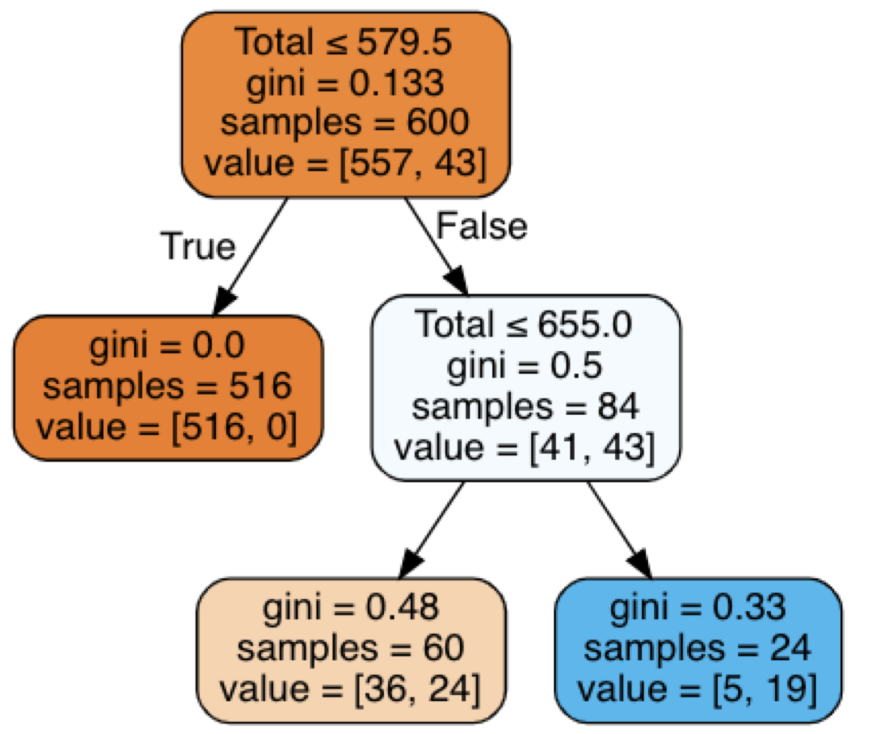
\includegraphics[height=20em]{./images/binary-classification-decision-tree.png}
\end{center}
\subsubsection{Prediction using decision tree}
\label{sec:org1d59fc6}
The confusion matrix is shown below. The \(x\)-axis represents the predicted values, and the \(y\)-axis represents the actual values.
\begin{center}
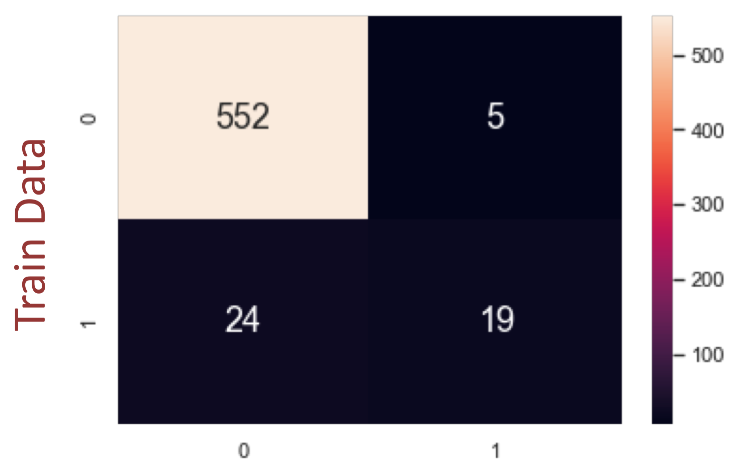
\includegraphics[width=.9\linewidth]{./images/binary-classification-training-data-prediction.png}
\end{center}
\subsection{Classification accuracy}
\label{sec:orgcb0699a}
\begin{itemize}
\item The classification accuracy is the fraction of correct predictions.
\begin{itemize}
\item A true positive (TP) is when true is predicted as true.
\item A true negative (TN) is when false is predicted as false.
\end{itemize}
\end{itemize}

It is given by:
\[\text{Classification accuracy} = \frac{\text{Number of true positives} + \text{Number of true negatives}}{\text{Total number of data points}}\]
\subsection{Classification errors}
\label{sec:org5f9cb08}
\begin{itemize}
\item A false negative (FN) is when true is predicted as false.
\item A false positive (FP) is when false is predicted as true.
\end{itemize}

\[fpr = \frac{\text{Number of false positives}}{\text{Number of false positives + Number of true negatives}}\]
\[fnr = \frac{\text{Number of false negatives}}{\text{Number of false negatives + Number of true positives}}\]
\subsubsection{Training data example}
\label{sec:orgb464e67}
\begin{center}
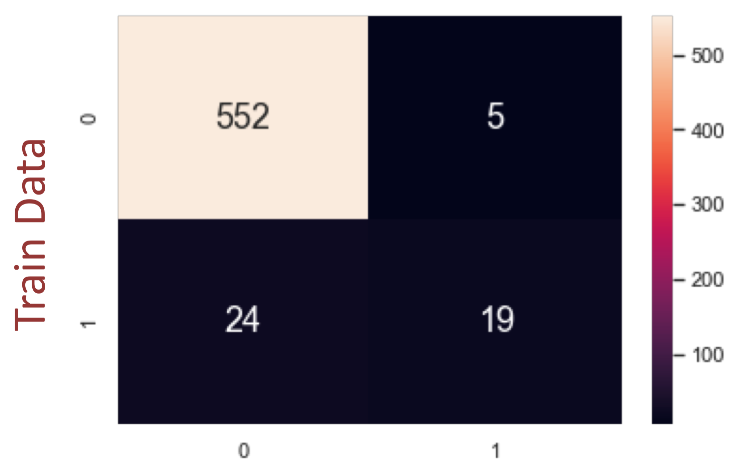
\includegraphics[width=.9\linewidth]{./images/binary-classification-training-data-prediction.png}
\end{center}
\[fpr = \frac{5}{557}, \quad fnr = \frac{24}{43}\]
\subsubsection{Test data example}
\label{sec:org30b710c}
\begin{center}
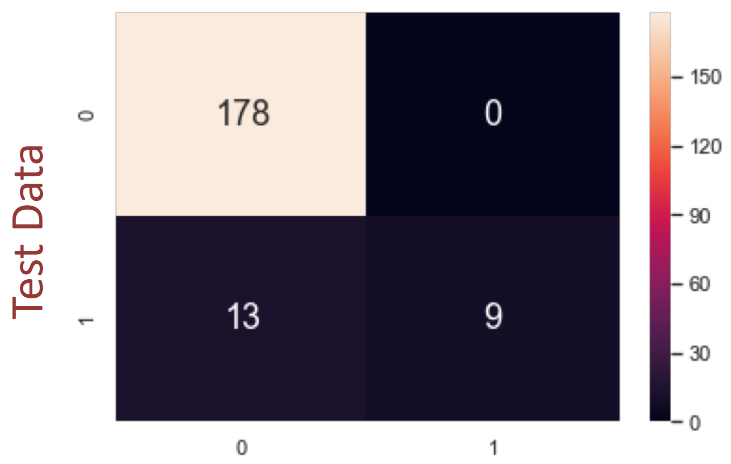
\includegraphics[width=.9\linewidth]{./images/binary-classification-test-data-prediction.png}
\end{center}
\[fpr = \frac{0}{178}, \quad fnr = \frac{13}{22}\]

 \newpage
\subsection{Two-level decision tree}
\label{sec:org4f82f87}
The two-level decision tree and its corresponding confusion matrix is shown below.
\begin{center}
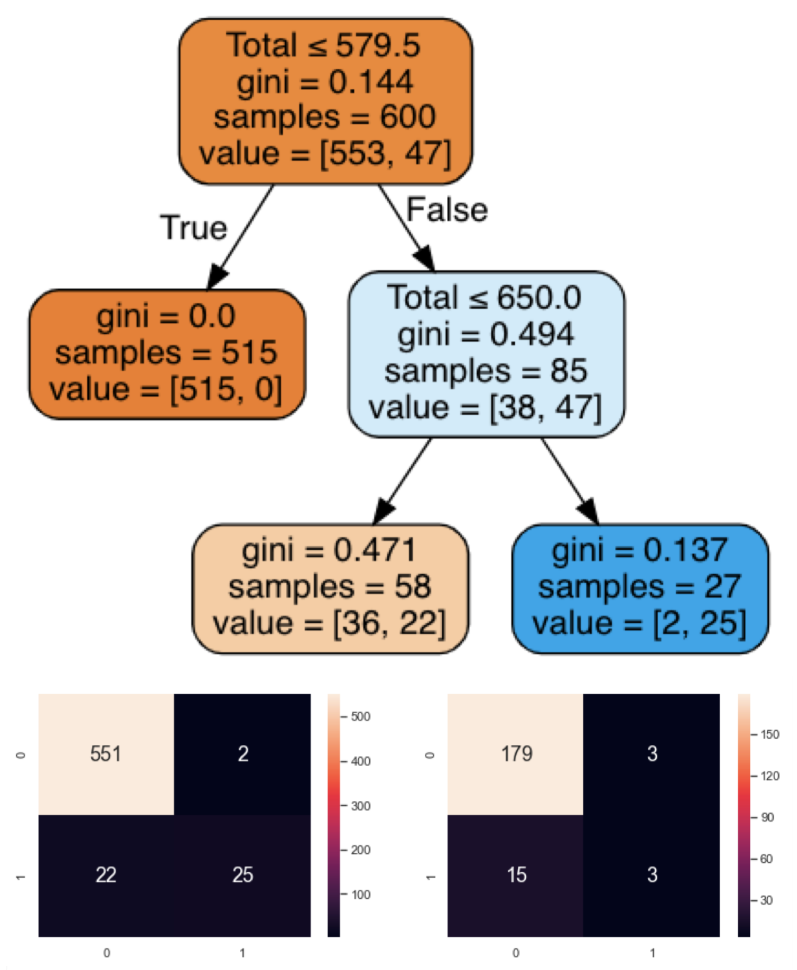
\includegraphics[width=.9\linewidth]{./images/binary-classification-two-level-decision-tree.png}
\end{center}

 \newpage
\subsection{Three-level decision tree}
\label{sec:org329d1ba}
The three-level decision tree and its corresponding confusion matrix is shown below.
\begin{center}
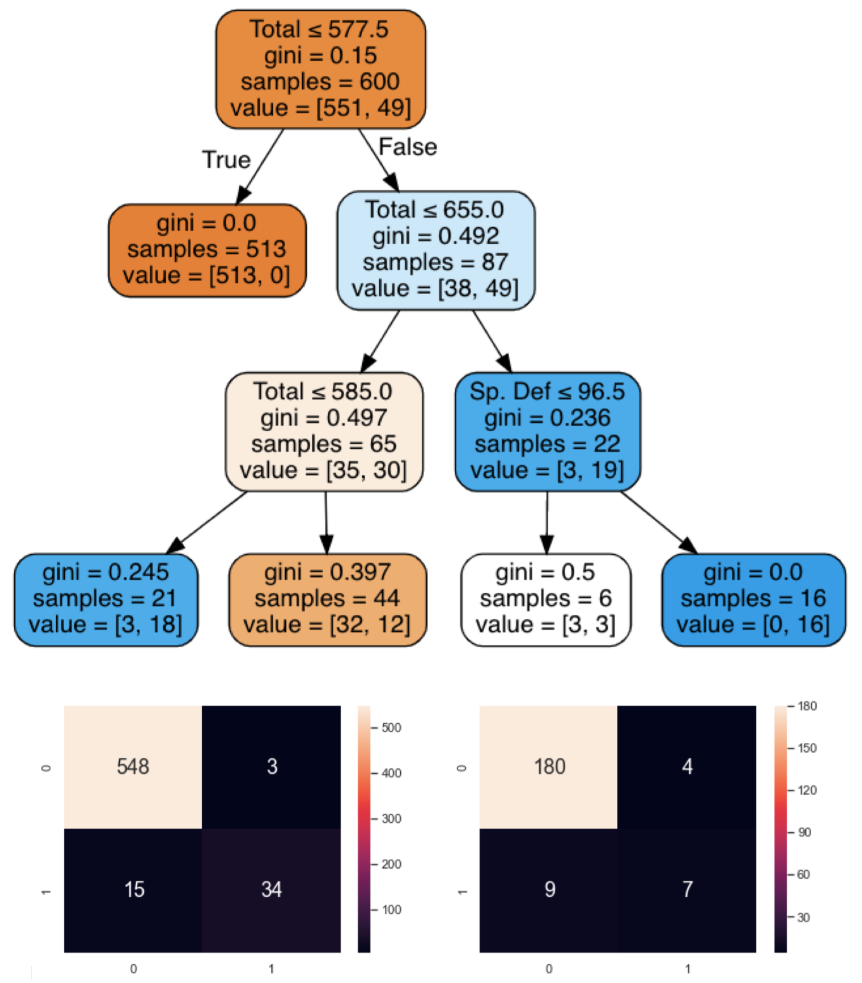
\includegraphics[width=.9\linewidth]{./images/binary-classification-three-level-decision-tree.png}
\end{center}
\section{Pattern recognition}
\label{sec:org703639a}
How to optimally learn from the data?
\begin{itemize}
\item Is there a pattern in the acquired data?
\item How to learn the underlying pattern?
\item How to exploit the pattern in the data?
\end{itemize}
\subsection{K-means clustering}
\label{sec:org4d05385}
\begin{itemize}
\item \textbf{K} is the potential number of clusters.
\item We will need to choose \textbf{K} cluster centroids from the data set, i.e. we will need to pick \textbf{K} number of points in the data set that is roughly in the middle of a cluster, to initialise the model.
\item For each point in the data set, relabel the point according to the nearest centroid.
\item For each cluster of data points, recompute the centroid of the cluster.
\end{itemize}

\begin{center}
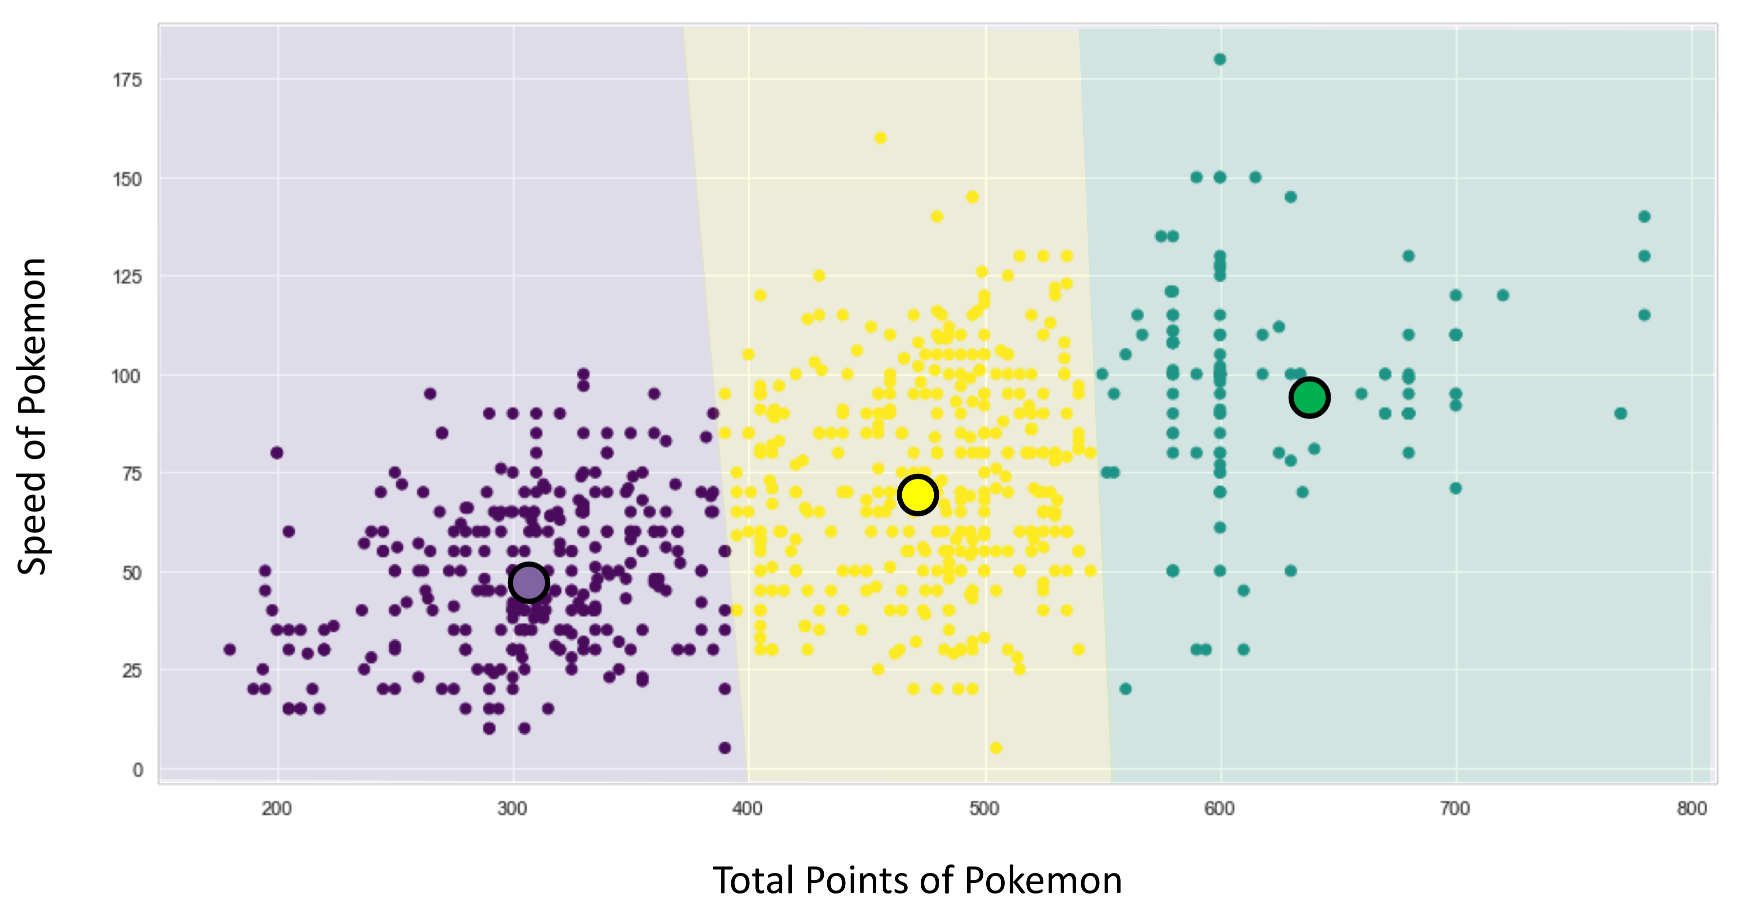
\includegraphics[width=.9\linewidth]{./images/k-means-clustering-graph.png}
\end{center}

Machine learning questions:
\begin{itemize}
\item How many clusters are "visible"?
\item Can we identify those clusters?
\item What do the clusters signify?
\end{itemize}

Optimisation questions:
\begin{itemize}
\item What is the "optimal" cluster count?
\item Can we justify the cluster count?
\item What is a nice clustering metric?
\end{itemize}
\subsubsection{Example}
\label{sec:org00c5ab6}
\begin{center}
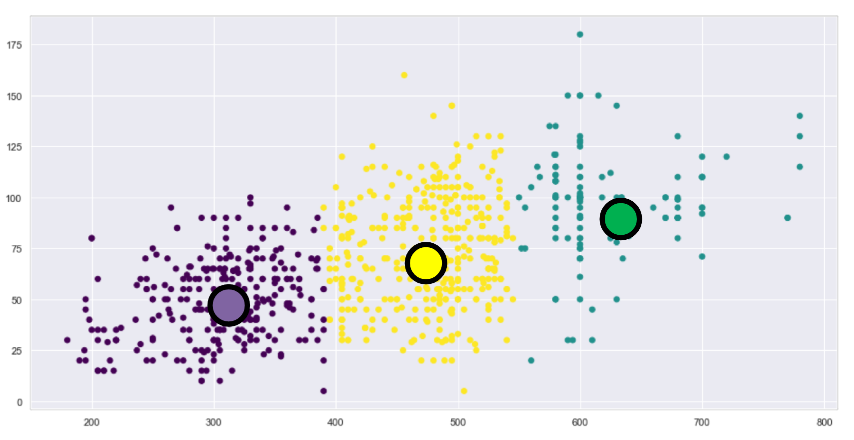
\includegraphics[width=.9\linewidth]{./images/k-means-clustering-example.png}
\end{center}

\begin{center}
\begin{tabular}{lrr}
Features & Total & Speed\\
\hline
Cluster 0 & 305.65 & 49.36\\
Cluster 1 & 622.57 & 97.08\\
Cluster 2 & 474.27 & 73.55\\
\end{tabular}
\end{center}

The within-cluster sum of squares is 2118651.

 \newpage
\subsubsection{Determining the optimal number of clusters}
\label{sec:orgac50b5c}
For the above data set:
\begin{center}
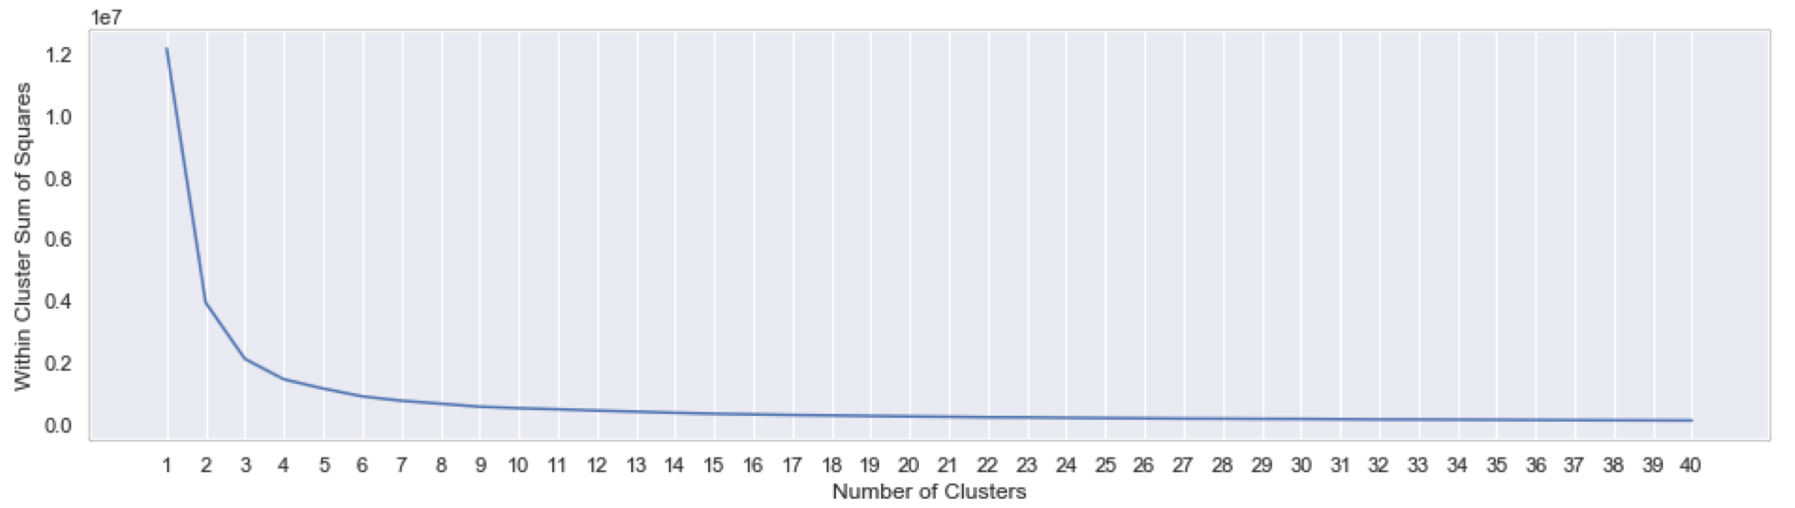
\includegraphics[width=.9\linewidth]{./images/within-cluster-sum-of-squares-graph.png}
\end{center}

The guess for the optimal number of clusters is 4.

\begin{center}
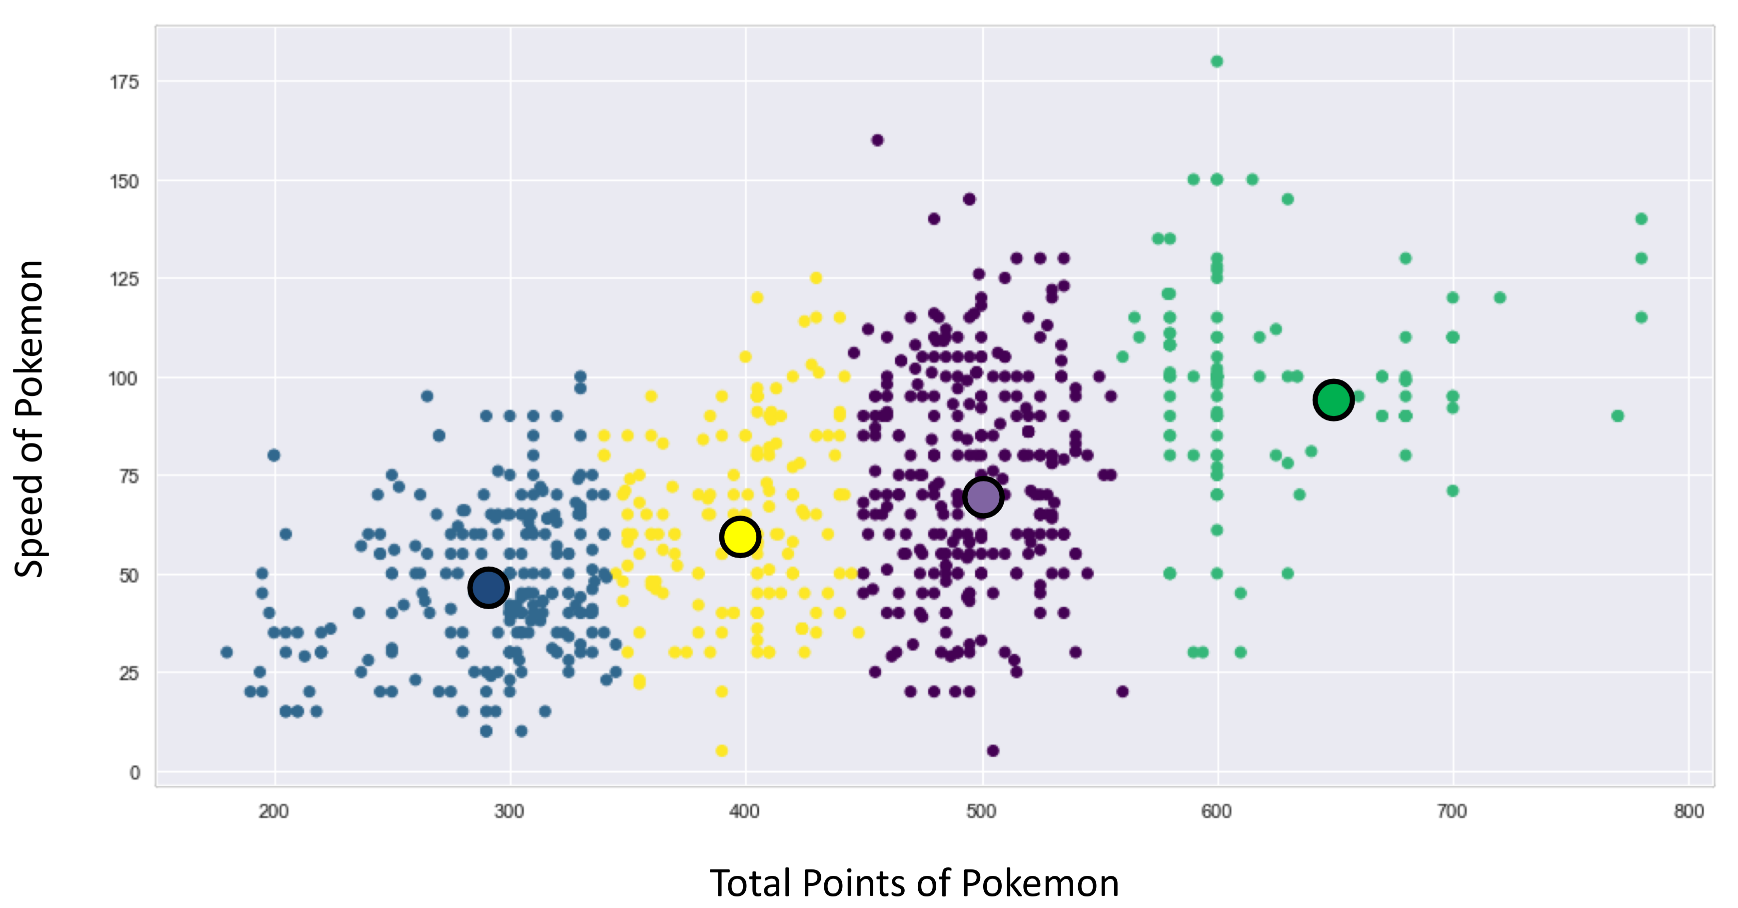
\includegraphics[width=.9\linewidth]{./images/result-of-optimal-number-of-clusters.png}
\end{center}

\begin{center}
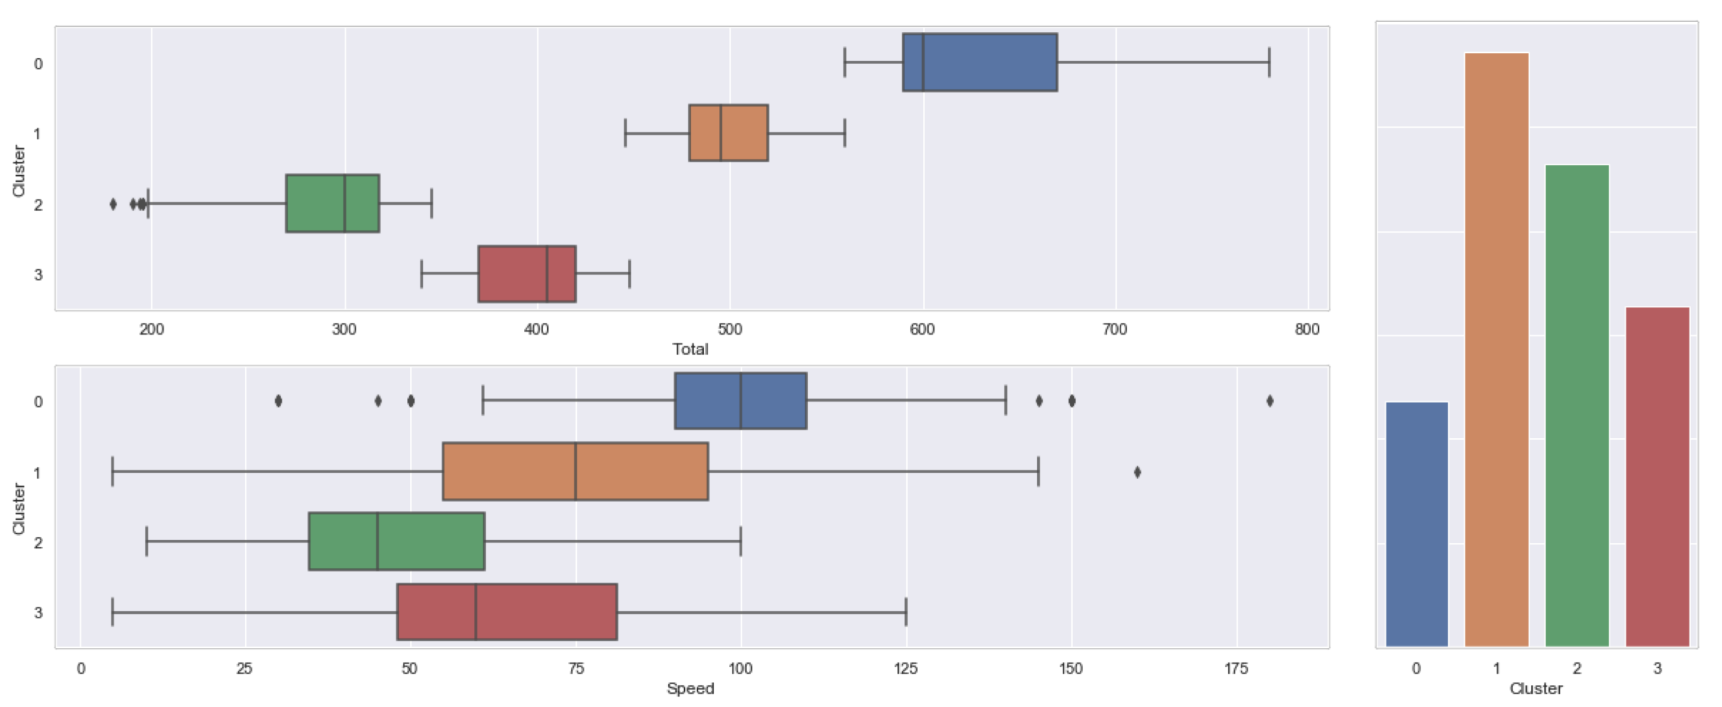
\includegraphics[width=.9\linewidth]{./images/box-plot-of-the-optimal-number-of-clusters.png}
\end{center}

 \newpage
\subsection{Local outlier factor (anomaly detection)}
\label{sec:orga9722a3}
\begin{itemize}
\item \textbf{K} is the total number of neighbours.
\item \textbf{d} is the fraction of anomalies in the data.
\item For each point in the dataset, find \textbf{K} nearest neighbours in the data, and compute if the density is high enough.
\item The density can be obtained by dividing the number of neighbours by the area on the plot, i.e.
\[\text{Density} = \frac{\text{Number of neighbours}}{\pi \left(\text{Radius of the circular area occupied} \right)^2}\]
\end{itemize}

\begin{center}
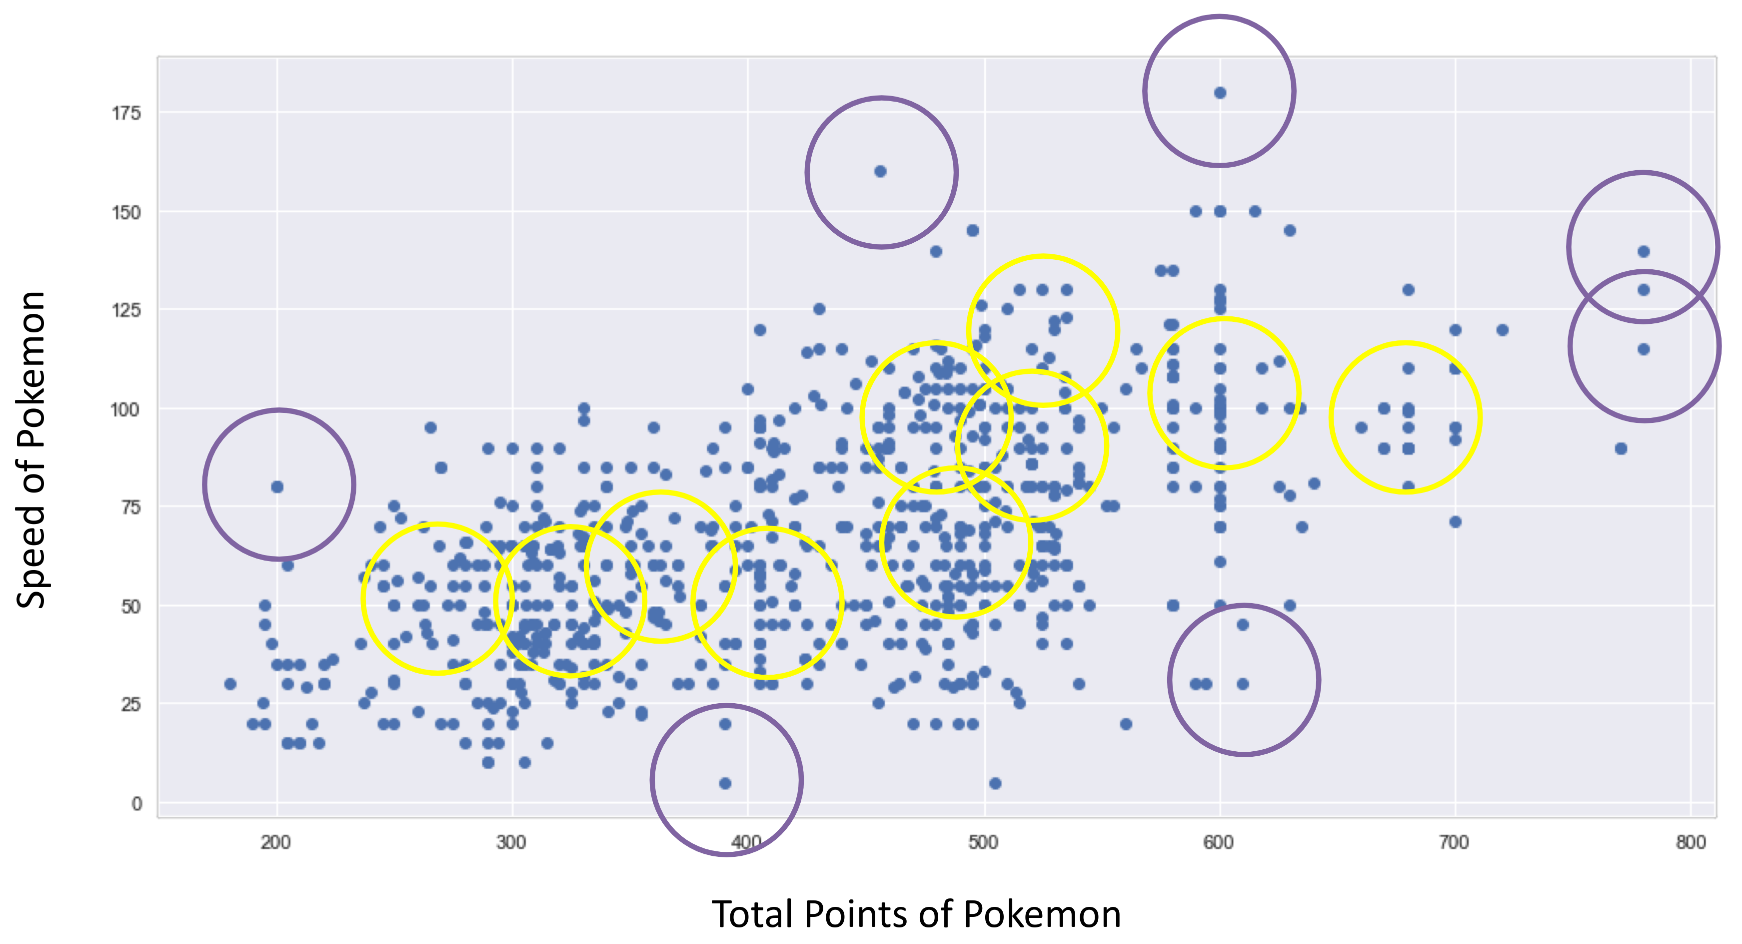
\includegraphics[height=12em]{./images/k-th-nearest-neighbours-graph.png}
\end{center}

\begin{center}
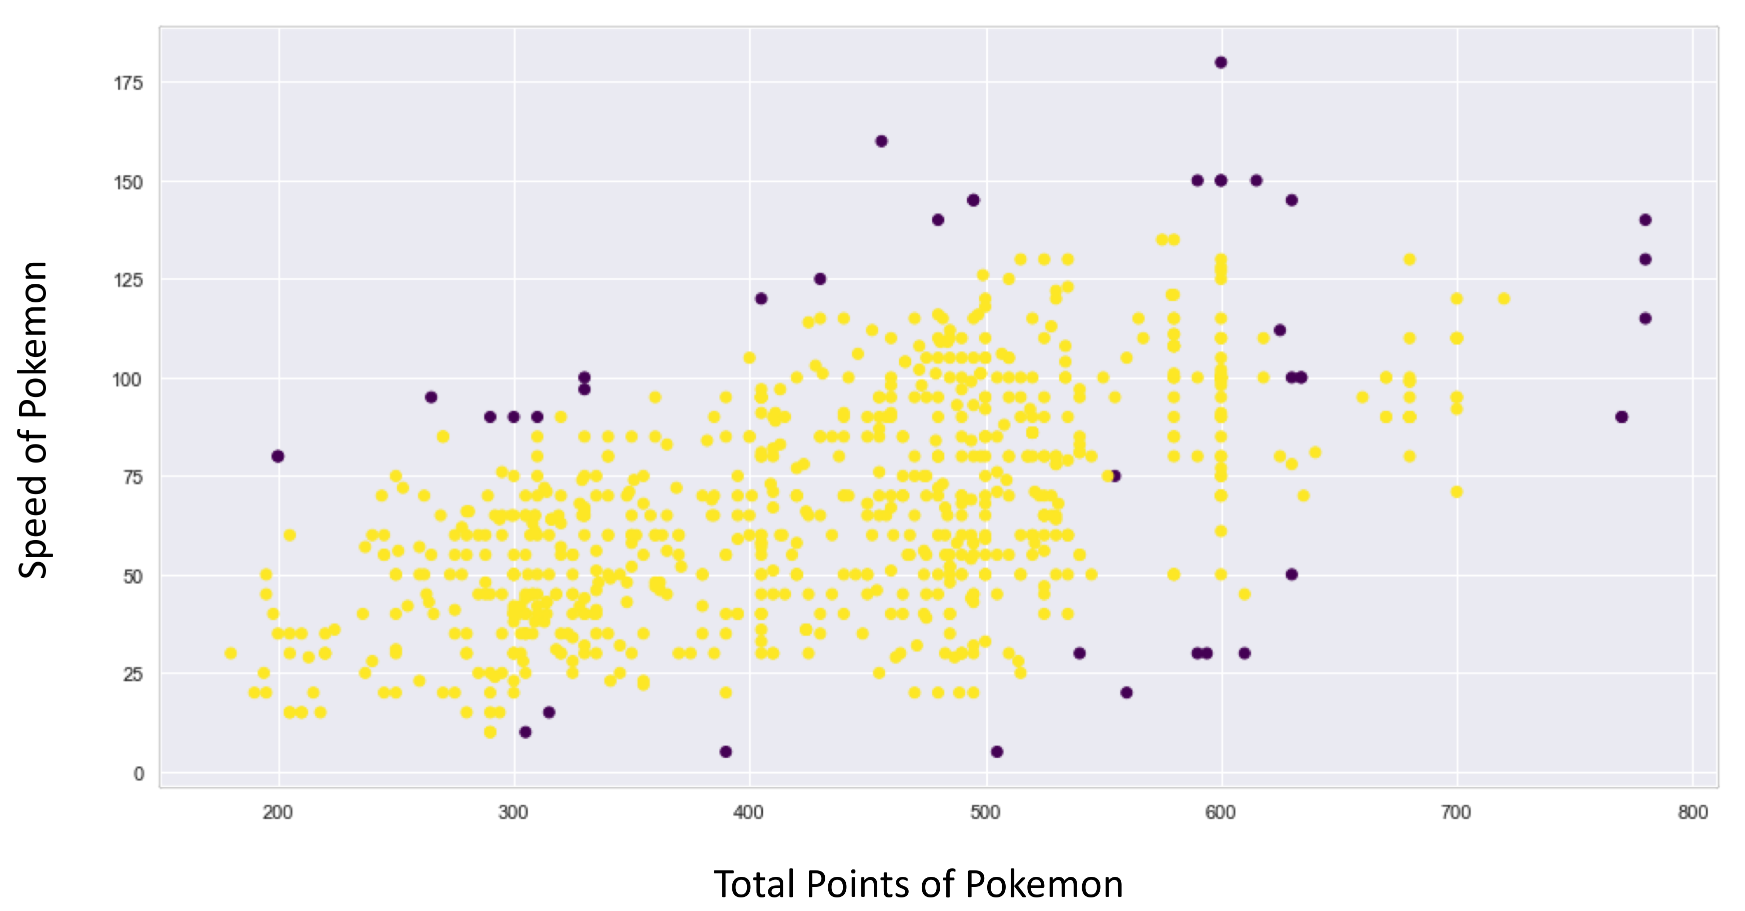
\includegraphics[height=12em]{./images/k-th-nearest-neighbours-result.png}
\end{center}

Machine learning questions:
\begin{itemize}
\item How many anomalies are "visible"?
\item Can we identify those anomalies?
\item What do the anomalies signify?
\end{itemize}
\section{Data visualisation}
\label{sec:org7bfcce9}
How to present data in the most engaging way?
\begin{itemize}
\item Is there a "story" hidden in your data?
\item How to use visuals as information?
\item How to tell the "story" effectively?
\end{itemize}

There are two goals when presenting data:
\begin{itemize}
\item Convey your story.
\item Establish credibility.
\end{itemize}
\subsection{Conveying your story}
\label{sec:org5613002}

\subsubsection{Effectiveness}
\label{sec:orgb26f1e9}
\begin{itemize}
\item A visualisation is more effective than another if the information conveyed by one visualisation is more \textbf{readily perceived} than the information in the other visualisation.
\item Use encodings that people decode more quickly and accurately.
\end{itemize}

\begin{center}
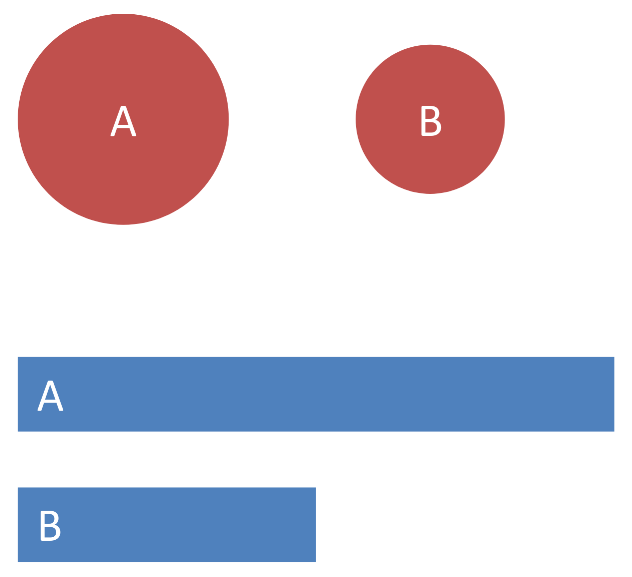
\includegraphics[height=20em]{./images/data-visualisation-effectiveness-diagram.png}
\end{center}
\subsection{Establish credibility}
\label{sec:org16a9743}

\subsubsection{Expressiveness}
\label{sec:org6d1a516}
\begin{itemize}
\item A set of facts is expressible in a visual language if the visualisations in the language express \textbf{all the facts} in the set of data, and \textbf{only the facts} in the data.
\item Tell the truth and nothing but the truth.
\item Do not lie, and do not lie by omission.
\end{itemize}

\begin{center}
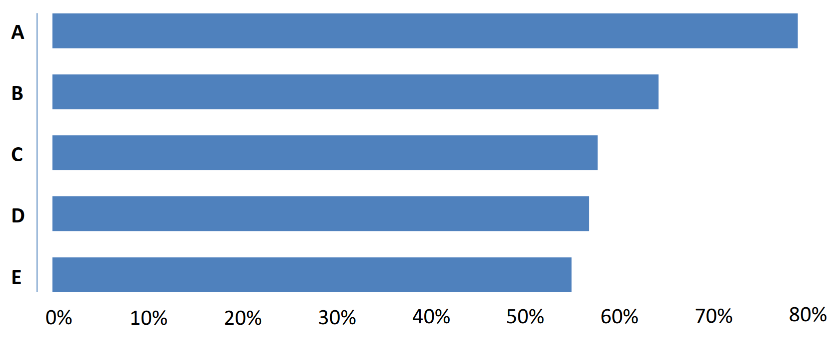
\includegraphics[width=.9\linewidth]{./images/data-visualisation-expressiveness-example-diagram.png}
\end{center}
\subsection{Good versus bad visualisations}
\label{sec:org223f764}
\begin{center}
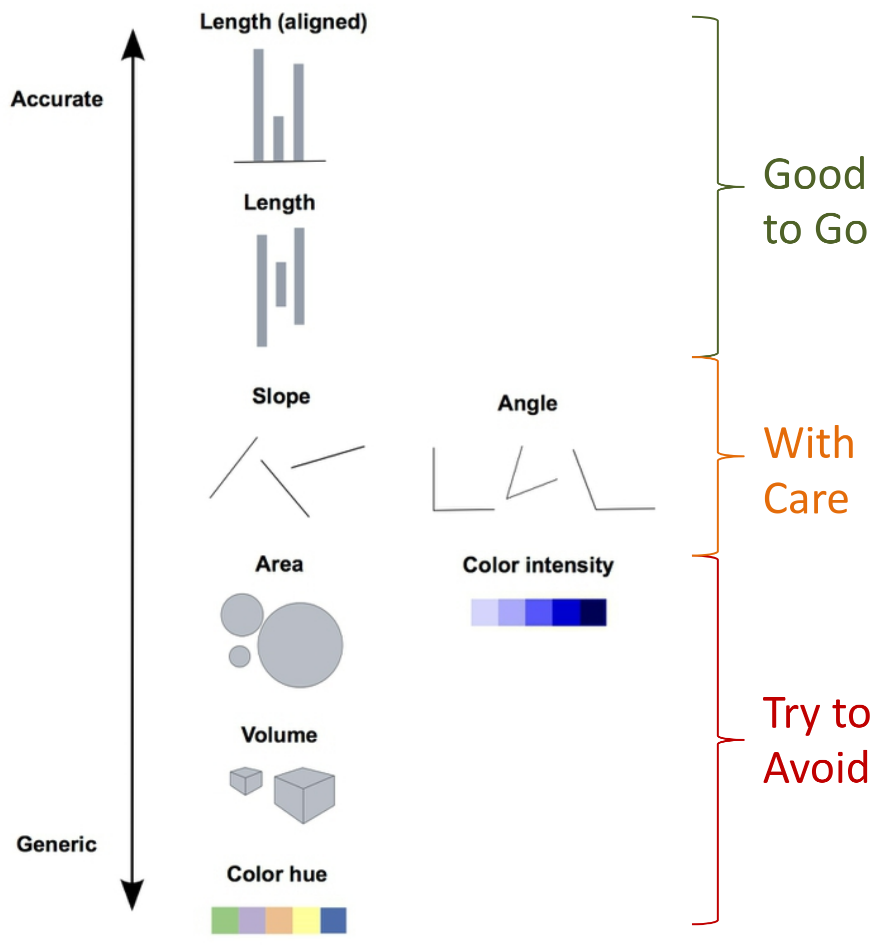
\includegraphics[width=.9\linewidth]{./images/good-vs-bad-visualisations.png}
\end{center}

 \newpage
\subsection{Data ink}
\label{sec:org68e0290}
Bold fonts and high contrast should be used to ensure that the data ink ratio is as high as possible.
\subsubsection{Good example}
\label{sec:org322fc2e}
\begin{center}
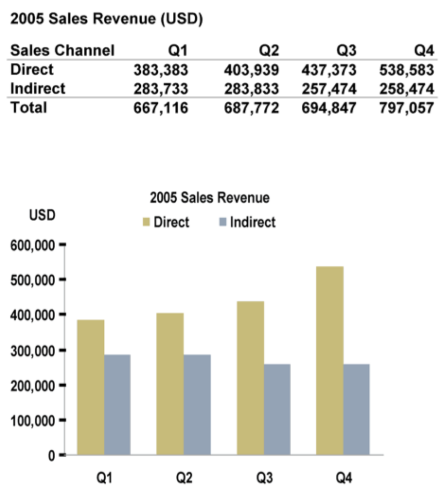
\includegraphics[width=.9\linewidth]{./images/data-ink-example.png}
\end{center}
\subsubsection{Bad example}
\label{sec:org46ce965}
\begin{center}
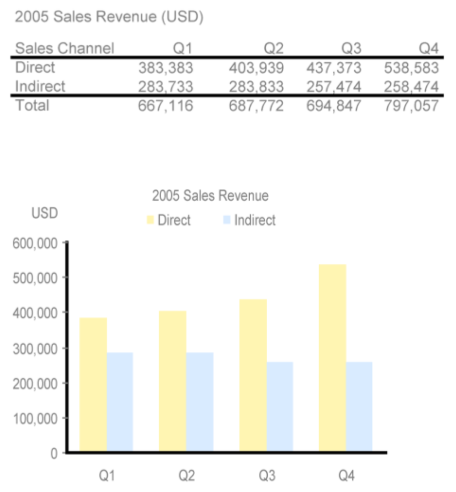
\includegraphics[width=.9\linewidth]{./images/non-data-ink-example.png}
\end{center}

 \newpage
\subsection{Interpretation}
\label{sec:orga44dd95}
Think about the context of your data and figure out the most effective way to present that data to your audience.

\begin{center}
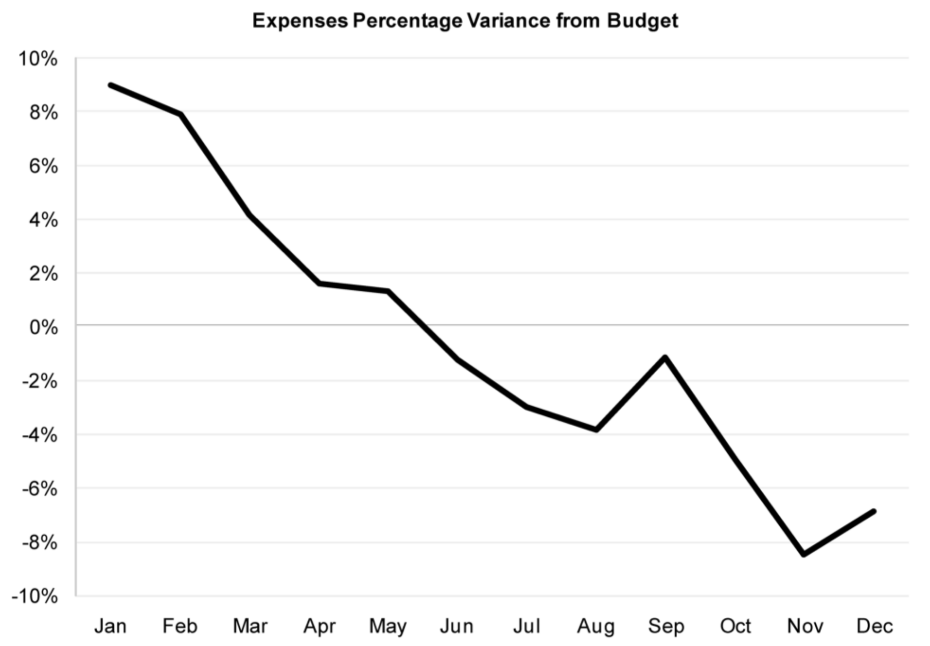
\includegraphics[width=.9\linewidth]{./images/interpretation-example.png}
\end{center}
\subsection{Visual vocabulary}
\label{sec:org9a96f2f}
\begin{center}
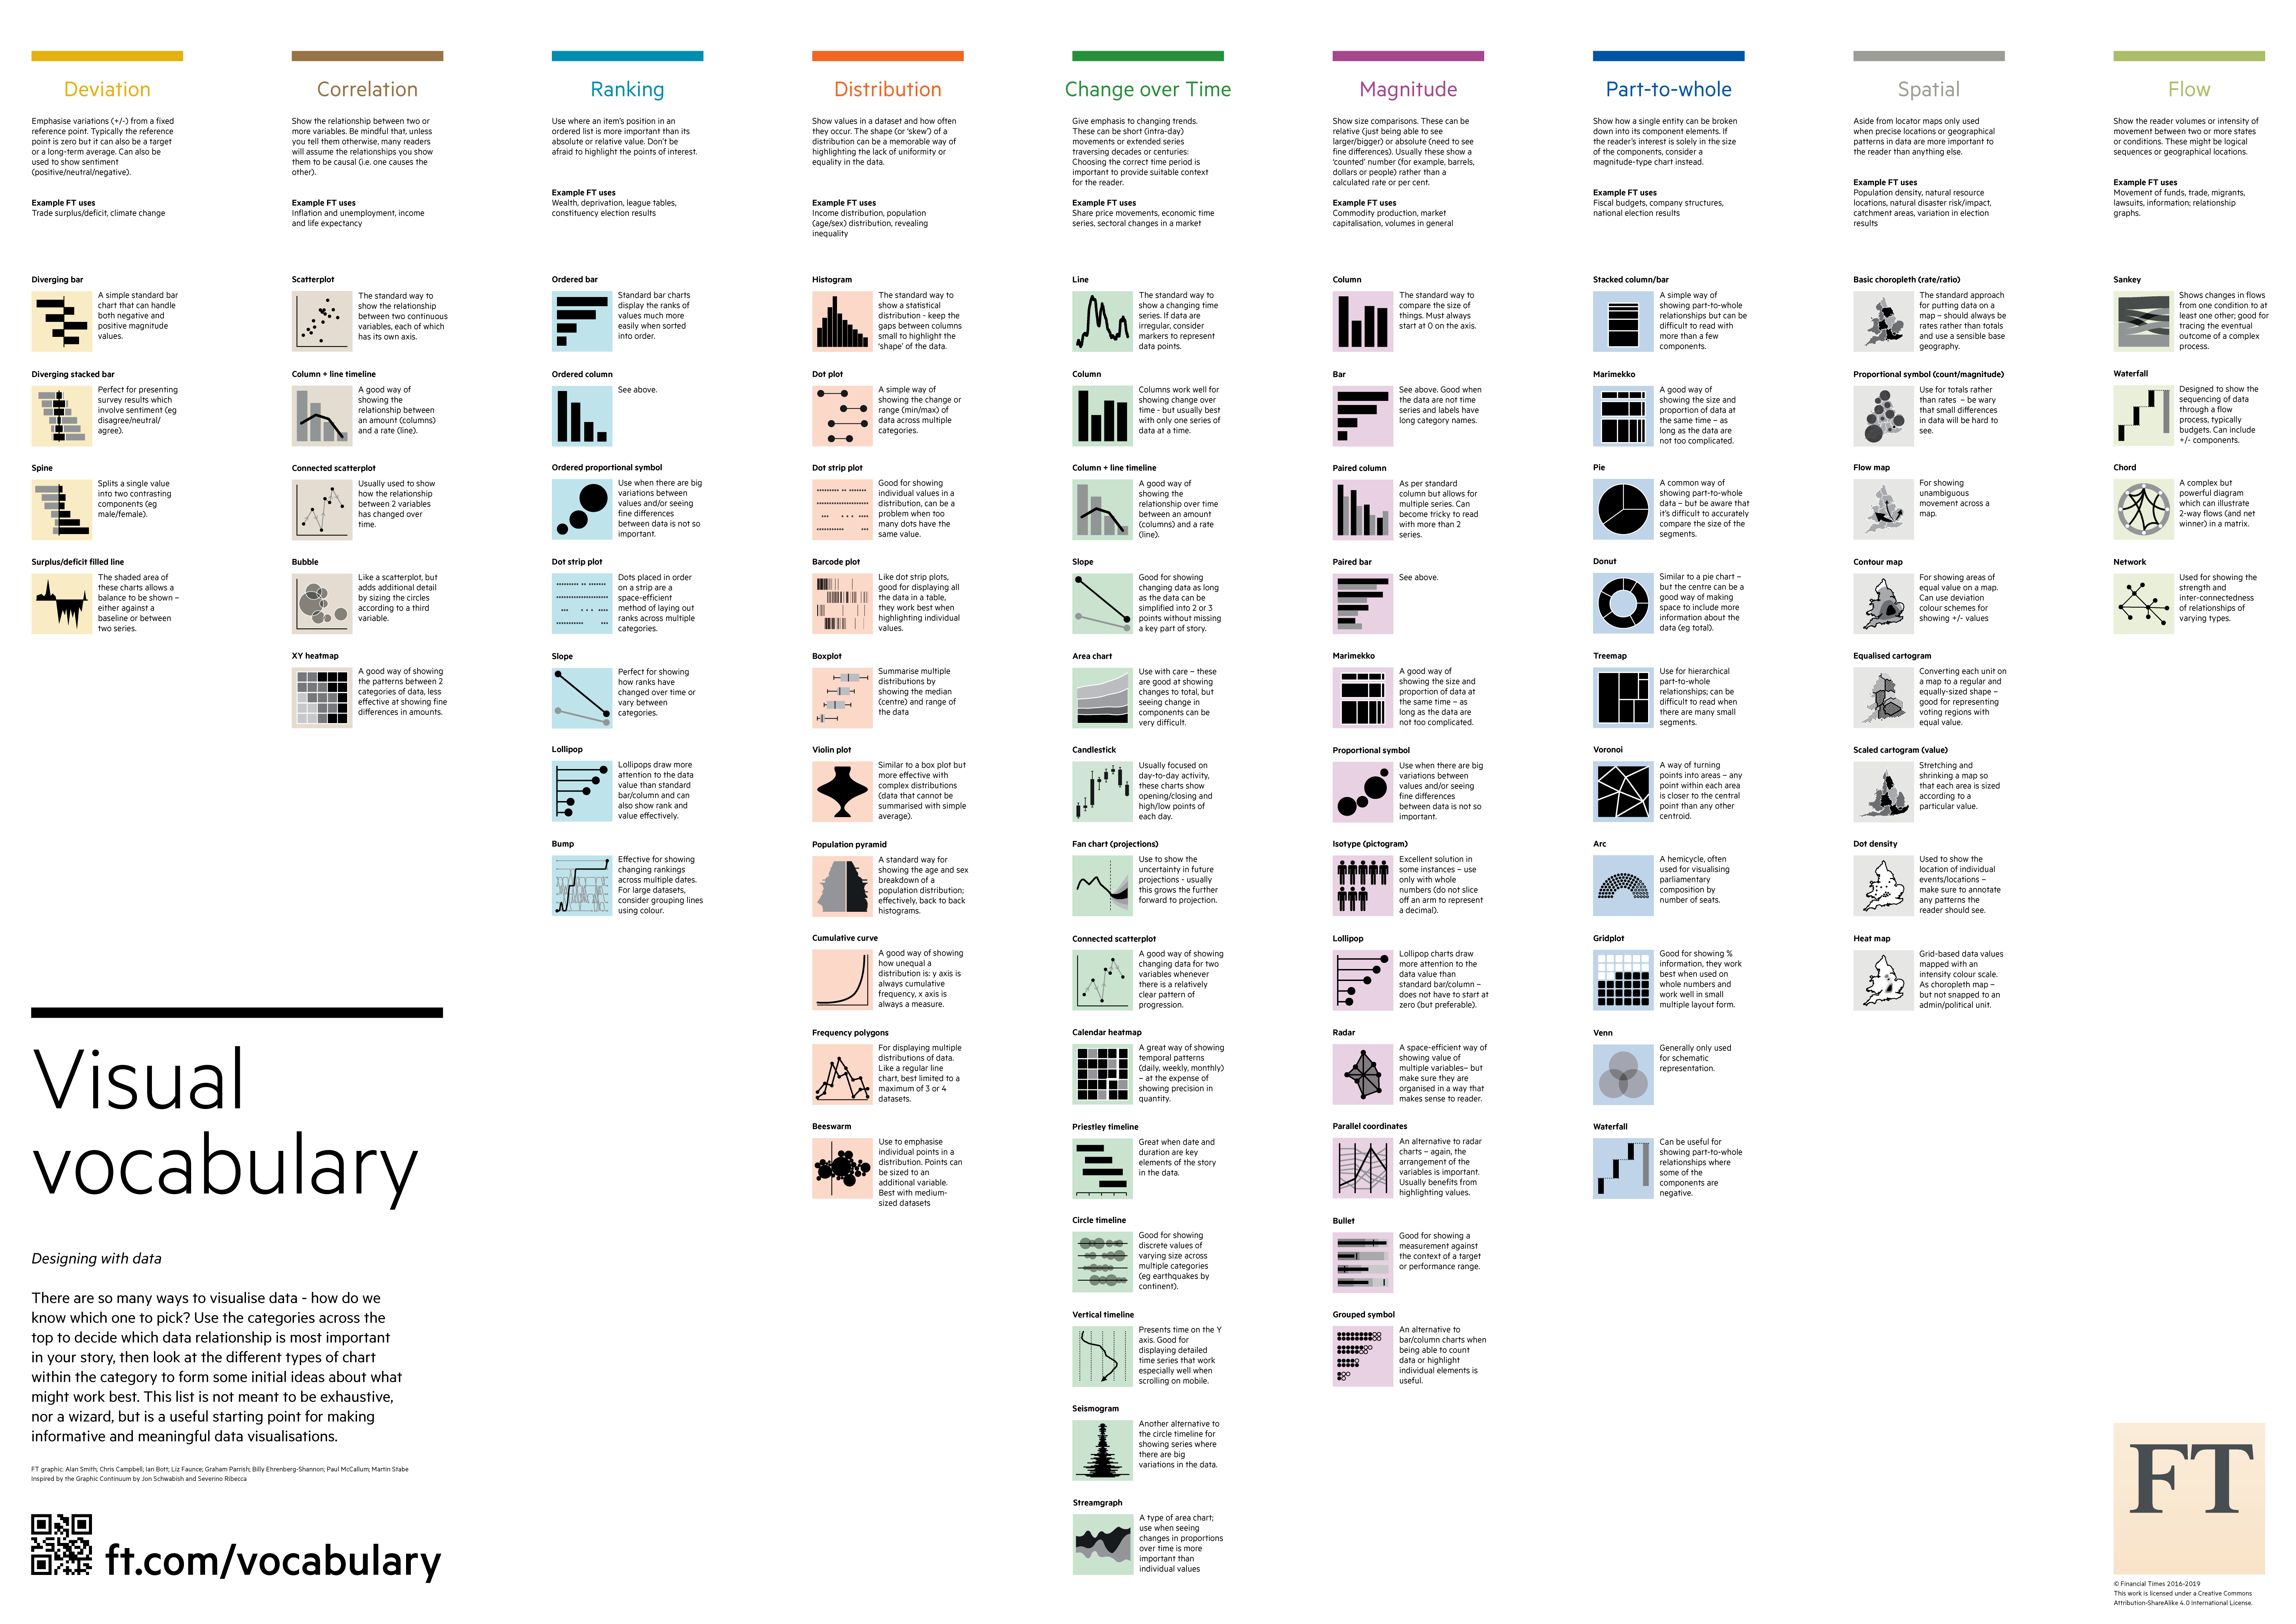
\includegraphics[width=.9\linewidth]{./images/visual-vocabulary.png}
\end{center}

 \newpage
\section{Introduction to artificial intelligence (AI)}
\label{sec:org23fcf09}
AI is intelligence demonstrated by machines, in contrast to the *natural intelligence (NI) displayed by humans and other animals.
\subsection{Founding fathers of AI}
\label{sec:orgb4827e7}
\begin{enumerate}
\item John MacCarthy
\item Marvin Minsky
\item Claude Shannon
\item Ray Solomonoff
\item Alan Newell
\item Herbert Simon
\item Arthur Samuel
\item Oliver Selfridge
\item Nathaniel Rochester
\item Trenchard More
\end{enumerate}
\subsection{Timeline}
\label{sec:org96495d8}
\begin{center}
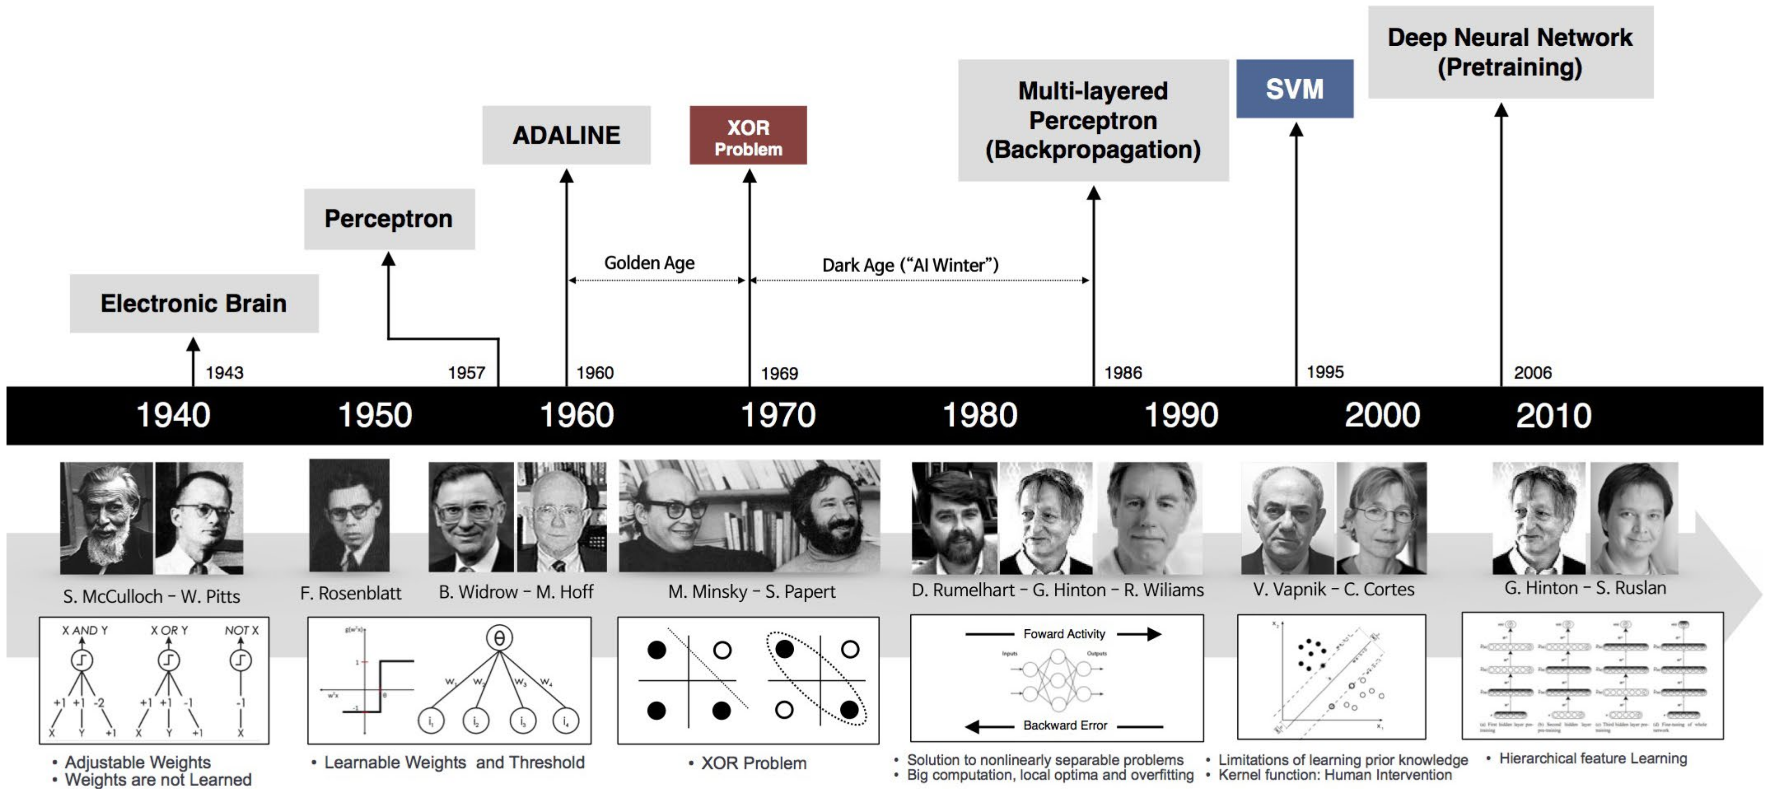
\includegraphics[width=.9\linewidth]{./images/timeline-of-ai-development.png}
\end{center}
\subsection{Views of AI}
\label{sec:org53638ec}
\begin{enumerate}
\item Thinking humanly
\item Acting humanly
\item Thinking rationally
\item Acting rationally
\end{enumerate}
\subsubsection{Thinking humanly: Cognitive Modelling}
\label{sec:orgab681dc}
\begin{itemize}
\item In the 1960s, there was a "cognitive revolution" with the advent of information-processing psychology.
\item It requires scientific theories of internal activities of the brain.
\item Both approaches (cognitive science and cognitive neuroscience) are now distinct from AI.
\end{itemize}
\subsubsection{Acting humanly: Turing test}
\label{sec:orga0b734a}
\begin{itemize}
\item Alan Turing created the Turing test in the 1950s, initially called the imitation game.
\item The aim is to test a machine's ability to exhibit intelligent behaviour equivalent to that of a human.
\item In the test, a human evaluator judges a text transcript of a natural-language conversation between a human and a machine.
\item The evaluator tries to identify the machine, and the machine passes if the evaluator cannot reliably tell them apart.
\item Suggested major components of AI: knowledge, reasoning, language understanding, learning.
\end{itemize}

 \newpage
\subsubsection{Thinking rationally: "Laws of Thought"}
\label{sec:org6e2217a}
\begin{itemize}
\item Aristotle: What are correct arguments and thought processes?
\begin{itemize}
\item Several Greek schools developed various forms of logic, which are notations and rules of derivation for thoughts and may or may not have proceeded to the idea of mechanisation.
\end{itemize}
\item Direct line through mathematics and philosophy to modern AI.
\item Problems:
\begin{itemize}
\item Not all intelligent behaviour is mediated by logical deliberation.
\item What is the purpose of thinking? What thoughts should I have?
\end{itemize}
\end{itemize}
\subsubsection{Acting rationally}
\label{sec:orgbd587e6}
\begin{itemize}
\item Rational behaviour is doing the right thing.
\item The right thing is the thing that is expected to maximise goal achievement, given the available information.
\end{itemize}
\subsection{AI beating humans}
\label{sec:org803988f}

\subsubsection{AlphaGo vs world Champions}
\label{sec:orgf2ad889}
\textbf{March 9 to 15, 2016 (Lee Sedol)}
\begin{itemize}
\item Time limit: 2 hours
\item Venue: Seoul Four Seasons Hotel
\item AlphaGo wins (4:1)
\end{itemize}

\textbf{May 23 to 27, 2017 (Ke Jie)}
\begin{itemize}
\item Venue: Wuzhen, China
\item AlphaGo Wins (3:0)
\end{itemize}
\subsubsection{Libratus vs world champions}
\label{sec:org345abfb}
\begin{itemize}
\item Libratus is the first AI to defeat top human poker players.
\item The competition was held in 2017, from January 11 to 31, in Pittsburgh, with 120,000 hands being dealt.
\item It has nothing to do with deep learning, but it represents algorithms for solving large-scale games.
\end{itemize}
\subsection{Examples of natural language processing devices}
\label{sec:org6ee1ad5}
\begin{itemize}
\item Mi Box Voice Assistant
\item Google Assistant
\item Amazon Alexa
\end{itemize}
\subsection{Artificial intelligence for finance}
\label{sec:org570466a}
\begin{center}
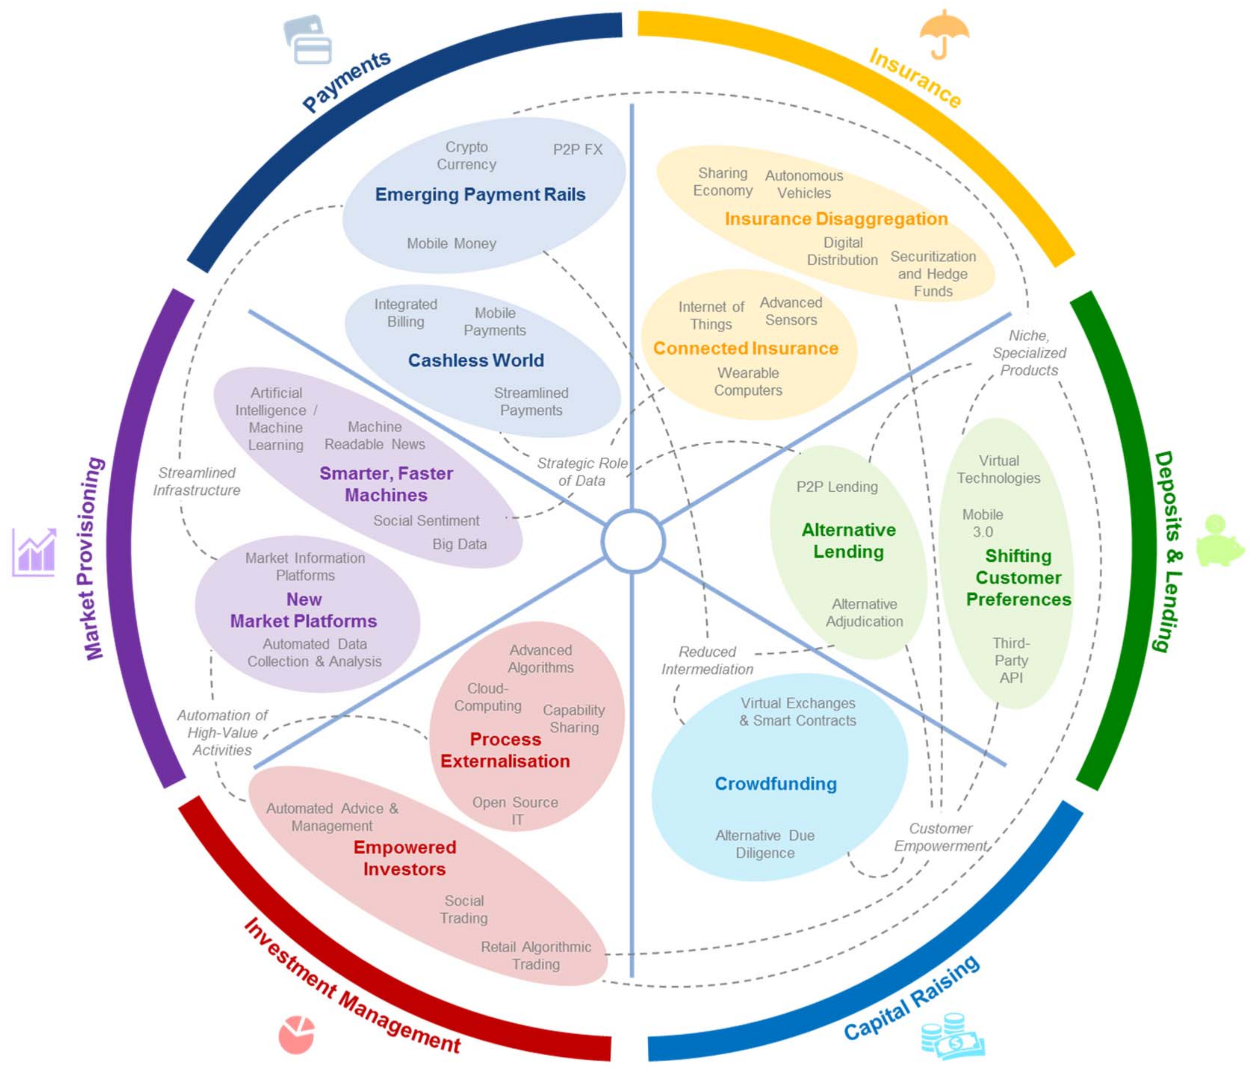
\includegraphics[width=.9\linewidth]{./images/artificial-intelligence-for-finance.png}
\end{center}
\subsection{What's next in AI for games?}
\label{sec:org520f1c5}
\begin{itemize}
\item Stochastic, open environment
\item Multiple players
\item Sequential decision, online
\item Strategic (selfish) behaviour
\item Distributed optimisation
\end{itemize}

 \newpage
\section{State of the art in data science and artificial intelligence}
\label{sec:org68cf77d}

\subsection{What is artificial intelligence?}
\label{sec:org3ac58ec}
\begin{itemize}
\item Artificial intelligence consists of 4 aspects:
\begin{itemize}
\item Thinking
\item Perception
\item Action
\item Reasoning
\end{itemize}
\item To create artificial intelligence is to build computer programs with algorithms that have the representation of the models targeted at thinking, perception, action and reasoning.
\end{itemize}
\subsection{History of artificial intelligence}
\label{sec:orgd3d1bab}

\subsubsection{1943}
\label{sec:org60a200f}
Warren McCulloch and Walter Pitts created the first artificial neural model, based on the human neuron.

\begin{center}
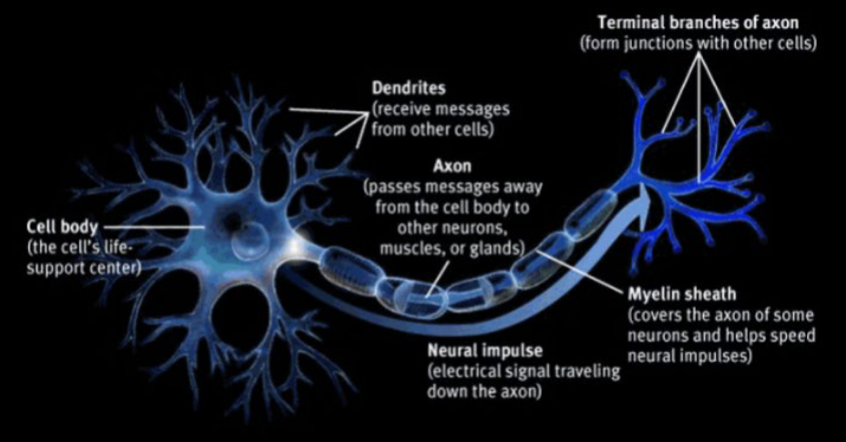
\includegraphics[width=.9\linewidth]{./images/human-neuron.png}
\end{center}

 \newpage
\subsubsection{World War II (1939 - 1945)}
\label{sec:org2f0697e}
During World War II, the Enigma machine was built to encrypt and decrypt communications.

\begin{center}
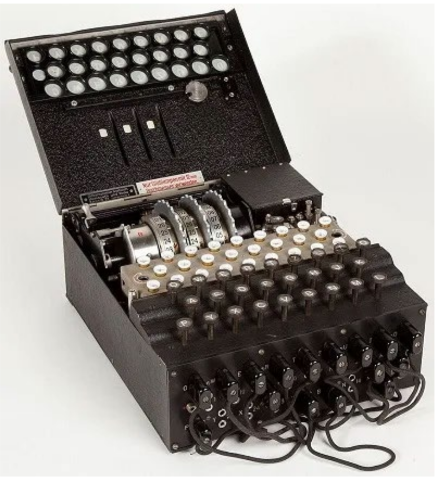
\includegraphics[height=15em]{./images/enigma-machine.png}
\end{center}
\subsubsection{1950}
\label{sec:org5c47a77}
Alan Turing, the father of modern computer science, created the Turing machine.

\begin{center}
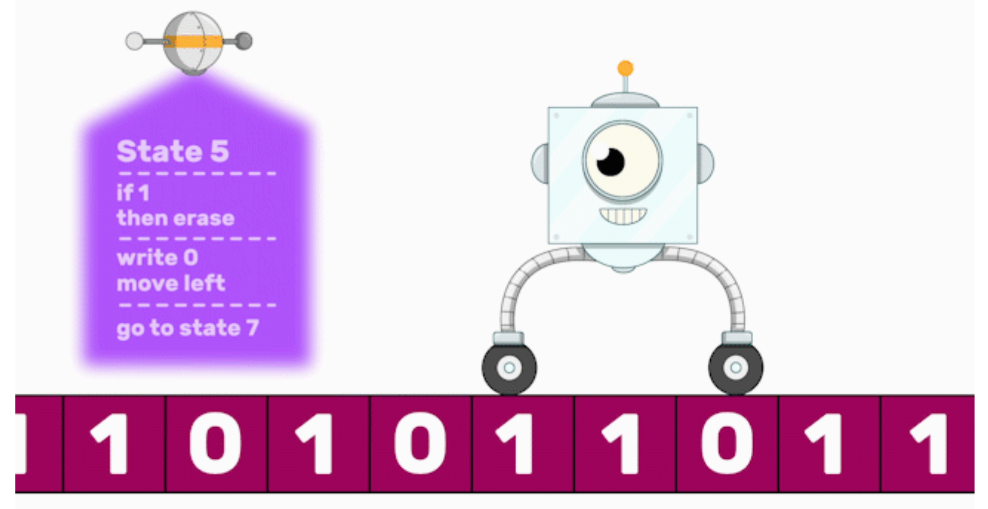
\includegraphics[width=.9\linewidth]{./images/turing-machine-graphic.png}
\end{center}

 \newpage
\subsubsection{1950s}
\label{sec:org2522679}
Early AI programs include:
\begin{itemize}
\item Arthur Samuel's Checkers Program
\item Newell and Simon's Logic Theorist
\item Gelernter's Geometry Theorem Prover
\end{itemize}
\subsubsection{1956 Darthmouth Conference}
\label{sec:orga18c918}
The 1956 Darthmouth Conference was attended by:
\begin{itemize}
\item Nathaniel Rochester
\item Marvin Minsky
\item John McCarthy
\item Oliver Selfridge
\item Ray Solomonoff
\item Trenchard More
\item Claude Shannon
\end{itemize}
\subsubsection{1957}
\label{sec:orge218bfa}
Frank Rosenblatt's created the perceptron, which was a device with the ability to learn.
\subsubsection{1961}
\label{sec:orgaf7ec7a}
The paper "Steps Toward Artificial Intelligence" was published by Marvin Minsky, talking about the possible uses of AI, such as:
\begin{itemize}
\item Search
\item Pattern recognition
\item Learning
\item Planning
\item Induction
\end{itemize}
\subsubsection{The Golden Years (1960 - 1974)}
\label{sec:org4159e77}
\begin{itemize}
\item Robinson created a complete algorithm for logical reasoning.
\item Appearance of expert systems, which are explicit, rule-based programs.
\begin{center}
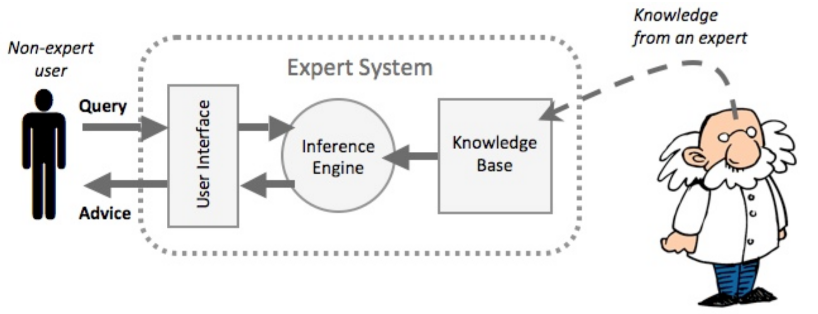
\includegraphics[width=.9\linewidth]{./images/expert-system-diagram.png}
\end{center}
\item Marvin Minsky's book, "Perceptrons", showed the limitations of simple neural networks in 1969.
\end{itemize}
\subsubsection{The first AI winter (1974 - 1980)}
\label{sec:orgd246945}
The first AI winter was mainly due to:
\begin{itemize}
\item Low computational power.
\item Results being primarily for toy problems.
\item Loss of government funding in AI.
\end{itemize}

 \newpage
\subsubsection{The second AI spring (1980 - 1988)}
\label{sec:org6d92cc9}
Japan created the Fifth Generation Computer Project (FGCP)
\begin{itemize}
\item It is a new generation of computers for "knowledge processing".
\item They were expert systems used in businesses with specialised hardware.
\end{itemize}

\begin{figure}[htbp]
\centering
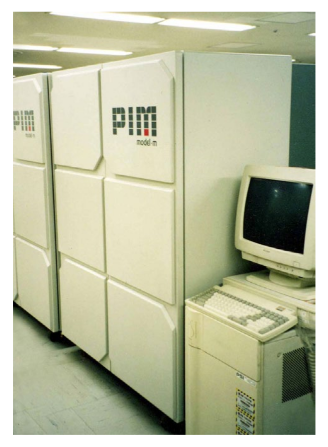
\includegraphics[height=30em]{./images/parallel-inference-machine.png}
\caption{Parallel Inference Machine in the 1980s}
\end{figure}

 \newpage
\subsubsection{The second AI winter (1988 - 1993)}
\label{sec:org6ba3830}
The second AI winter was due to:
\begin{itemize}
\item The goals of the Fifth Generation Computer Project being too ambitious.
\item Marvin Minsky talking about the coming of the AI winter.
\item Funding for AI ceasing.
\item Personal computers becoming popular.
\begin{center}
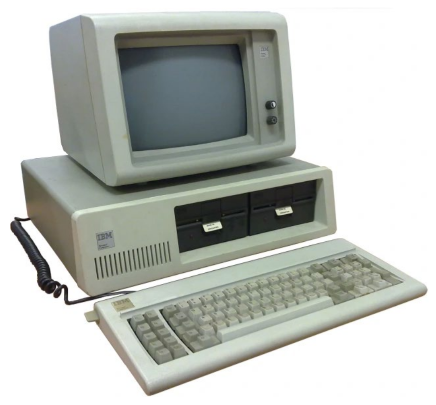
\includegraphics[height=20em]{./images/pc-in-the-1980s.png}
\end{center}
\end{itemize}
\subsubsection{AI comeback (1994 - 2000)}
\label{sec:org909213d}
\begin{itemize}
\item Resurgence of probability theories and focus on uncertainty.
\item IBM's Deep Blue defeated Chess World Champion Garry Kasparov in chess.
\item Moore's Law, which states that the number of transistors in an integrated circuit doubles every two years.
\end{itemize}
\subsubsection{The quiet years (2001 - 2012)}
\label{sec:org957e622}
\begin{itemize}
\item Internet boom.
\item Focus on big data and statistical techniques.
\item Graphics Processing Units (GPU) were created.
\item AI is used for narrow use cases, such as:
\begin{itemize}
\item 2005: Autonomous driving in the desert
\item 2011: IBM's Watson won Jeopardy
\item 2012: Convolutional Neural Networks (CNN) excelled at image recognition
\end{itemize}
\end{itemize}
\subsubsection{2012}
\label{sec:org9e743d9}
AlexNet wins the ImageNet competition, marking the resurgence of neural networks in computer vision.
\subsubsection{2014}
\label{sec:orgbae2d99}
Ian Goodfellow introduces Generative Adversarial Networks (GANs), revolutionising image generation.
\subsubsection{2015}
\label{sec:org86878b8}
Google DeepMind's AlphaGo beats the European Go champion, a milestone in game-playing AI.
\subsubsection{2016}
\label{sec:orgd2d3e00}
Google DeepMind introduces WaveNet, a deep generative model for generating raw audio waveforms.
\subsubsection{2017}
\label{sec:orge977868}
The paper "Attention Is All You Need" by Google introduces the transformer model, revolutionising natural language processing.
\subsection{GPT and Large Language Models}
\label{sec:org0c46ae0}
\begin{itemize}
\item AI has evolved from simple rule-based systems to complex models that understand and generate human language.
\item Generative Pre-trained Transformer (GPT) models are a series of AI models designed by OpenAI, showcasing significant advancements in machine learning.
\item Large Language Models (LLMs) like GPT are the cutting edge in natural language understanding and generation.
\end{itemize}
\subsubsection{Examples}
\label{sec:org1b53330}
\begin{itemize}
\item Midjourney
\item OpenAI's ChatGPT
\item DeepSeek AI
\item Dall-E 2
\item Google's Gemini
\item Microsoft and GitHub Copilot
\end{itemize}

 \newpage
\subsubsection{What is GPT?}
\label{sec:orgc8b4520}
\begin{itemize}
\item GPT models use transformer architecture, enabling them to efficiently process and generate language.
\item These models are "pre-trained" on vast amounts of text data, allowing them to understand context and produce relevant responses.
\item GPT's ability to generate coherent and contextually appropriate text has revolutionised AI's interaction with human language.
\item GPT 1 has 117 million parameters, GPT 2 has 1.5 billion parameters, and GPT 3 has 175 billion parameters.
\begin{center}
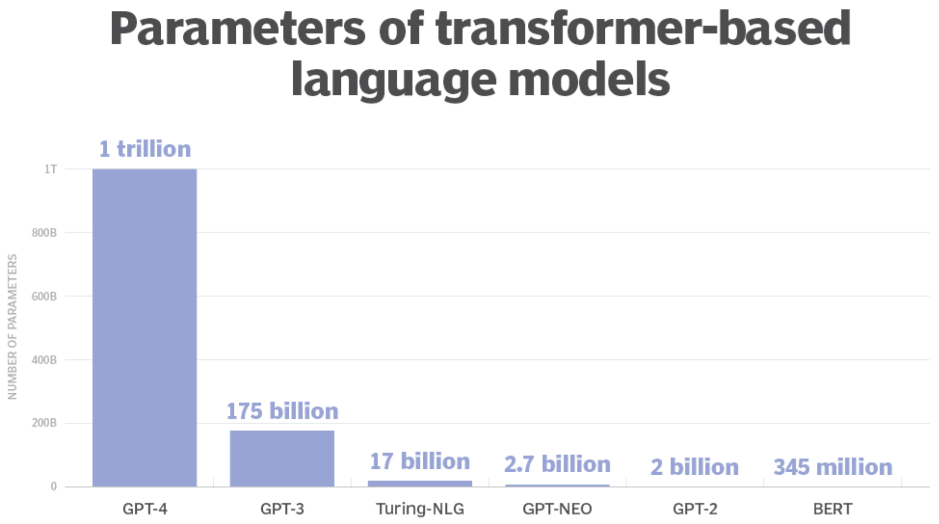
\includegraphics[width=.9\linewidth]{./images/parameters-of-transformer-based-language-models.png}
\end{center}
\end{itemize}

\begin{figure}[htbp]
\centering
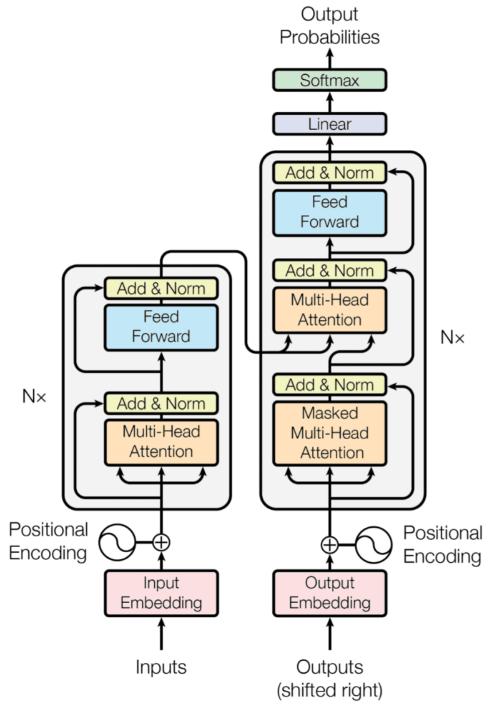
\includegraphics[height=40em]{./images/encoder-decoder-transformer-structure.png}
\caption{The encoder-decoder structure of the Transformer architecture.}
\end{figure}

 \newpage
\subsubsection{Limitations}
\label{sec:orgadf5876}
\begin{itemize}
\item Data bias, as GPT models can inherit biases present in their training data.
\item Computation cost, as training large models requires significant computation resources.
\item Ethical concerns, as there is potential for misuse in misinformation, privacy, and security.
\end{itemize}
\subsection{Features required for a machine to pass the Turing test}
\label{sec:orgdc66f04}
The features required for a machine to pass the Turing test are:
\begin{itemize}
\item Natural language processing (NLP), as NLP is required to communicate with the interrogator in general human language like English
\item Knowledge representation, as it is needed to store and retrieve information during the test.
\item Automated reasoning, which is needed to use the previously stored information for answering the questions.
\item Machine learning, which is needed to adapt new changes and can detect generalised patterns.
\item Vision (for total Turing test), which is needed to recognise the interrogator actions and other objects during a test.
\item Motor control (for total Turing test), which is needed to act upon objects if requested.
\end{itemize}

 \newpage
\section{Intelligent agents}
\label{sec:org48d830a}
An \textbf{agent} is an entity that \textbf{perceives} through sensors, like eyes, ears, cameras, and infrared range sensors, and \textbf{acts} through effectors, such as hands, legs and motors.

\begin{center}
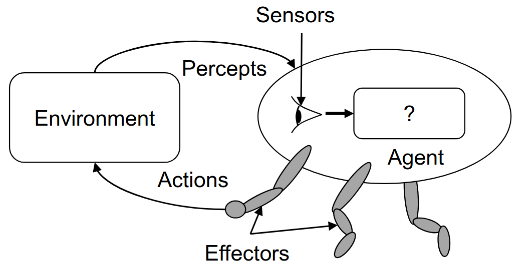
\includegraphics[width=.9\linewidth]{./images/agent-diagram.png}
\end{center}
\subsection{Rational agents}
\label{sec:org659cea3}
\begin{itemize}
\item A rational agent is one that does the \textbf{right} thing.
\end{itemize}
The rationality of the agent depends on:
\begin{itemize}
\item Performance measures.
\item Everything that the agent has perceived so far.
\item Built-in knowledge about the environment.
\item Actions that can be performed.
\end{itemize}
\subsubsection{Example: Google's X2 Driverless Taxi}
\label{sec:org53ce318}
\begin{itemize}
\item \textbf{Percepts}: Video, speed acceleration, engine status, GPS, radar, etc.
\item \textbf{Actions}: Steer, accelerate, brake, horn, display, etc.
\item \textbf{Goals}: Safety, arrive at destination, maximise profits, obey laws, passenger comfort, etc.
\item \textbf{Environment}: Singapore urban streets, highways, traffic, pedestrians, weather, customers, etc.
\end{itemize}
\subsubsection{Example: Medical diagnosis system}
\label{sec:org62a6ed9}
\begin{itemize}
\item \textbf{Percepts}: Symptoms, findings, patient's answers, etc.
\item \textbf{Actions}: Questions, medical tests, treatments, etc.
\item \textbf{Goals}: Healthy patient, faster recovery, minimise costs, etc.
\item \textbf{Environment}: Patient, hospital, clinic, etc.
\end{itemize}
\subsection{Autonomous agents}
\label{sec:org1ba6895}
\begin{itemize}
\item Autonomous agents do \textbf{not} rely entirely on the built-in knowledge about the environment, i.e. they are not entirely pre-programmed.
\item Otherwise, the agent will only operate successfully when the built-in knowledge is all correct.
\item Such agents adapt to the environment through experience.
\end{itemize}
\subsubsection{Example: Driverless car}
\label{sec:org8067171}
\begin{itemize}
\item Learning to drive in a driving centre.
\item Drive at NTU.
\item Drive on public roads.
\item Drive on highways.
\item Drive in City Hall.
\end{itemize}

 \newpage
\subsection{Simple reflex agents}
\label{sec:org521af11}
\begin{enumerate}
\item Find the \textbf{rule} whose condition matches the current situation, as defined by the percept.
\item Perform the action associated with that rule.
\end{enumerate}

\begin{center}
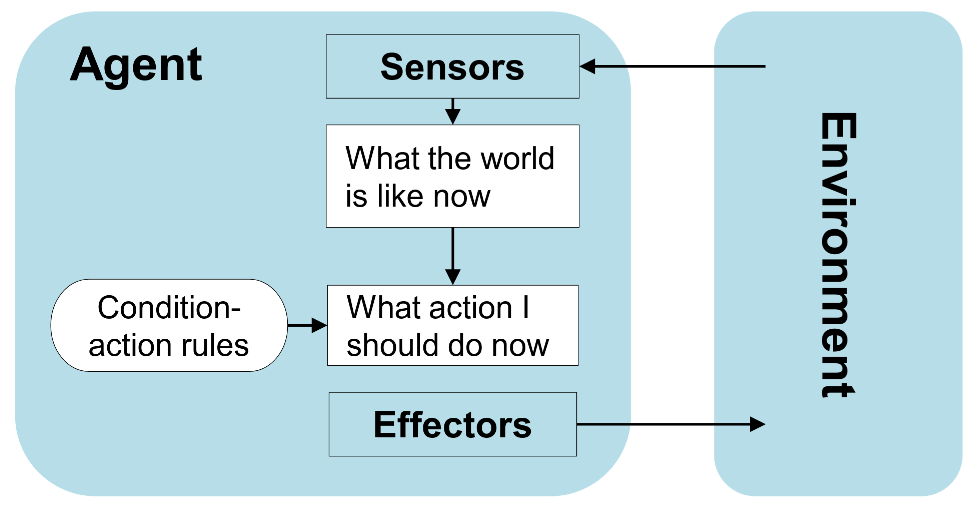
\includegraphics[height=14em]{./images/simple-reflex-agent-example.png}
\end{center}

For example, if the car in front is braking, then initiate braking.
\subsection{Reflex agent with state}
\label{sec:org149f81e}
\begin{enumerate}
\item Find the rule whose condition matches the current situation, as defined by the percept and the stored internal state.
\item Perform the action associated with that rule.
\end{enumerate}

\begin{center}
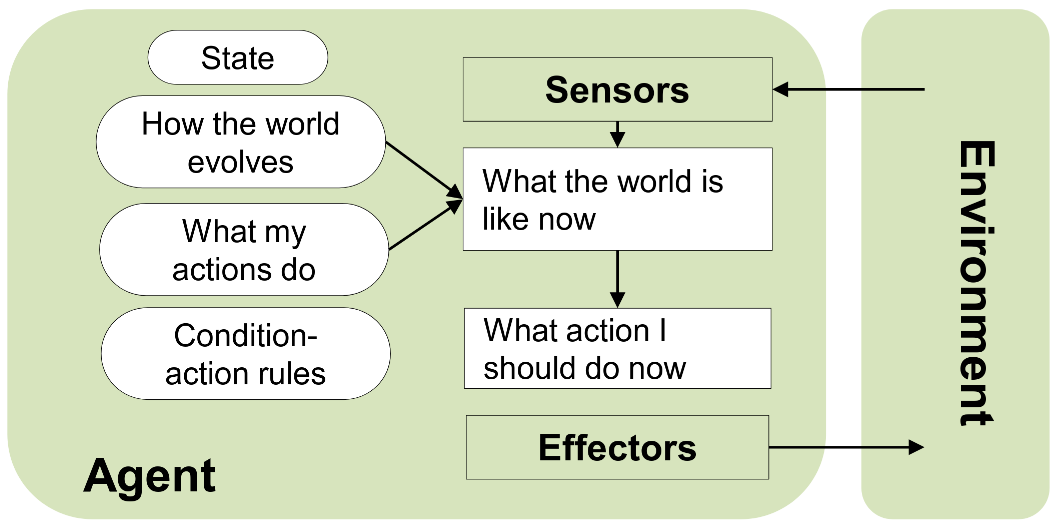
\includegraphics[height=14em]{./images/reflex-agent-with-state-diagram.png}
\end{center}

For example, if the agent was at NTU yesterday, and there is no traffic jam currently, then go to Orchard.
\subsection{Goal-based agents}
\label{sec:org5e91085}
Goal-based agents need some sort of goal information.

\begin{center}
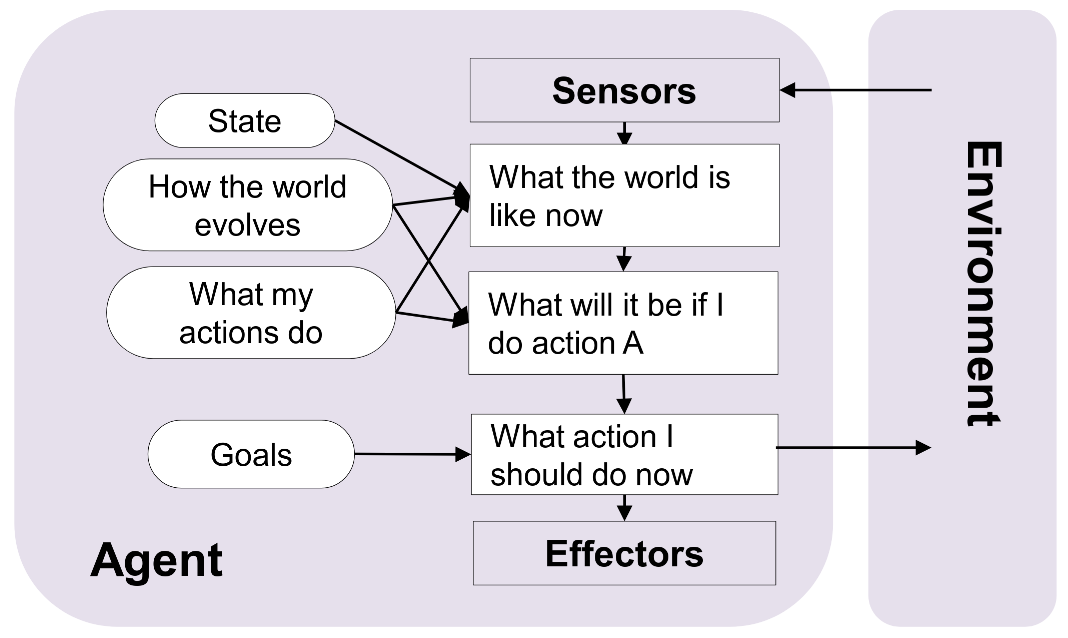
\includegraphics[width=.9\linewidth]{./images/goal-based-agent-diagram.png}
\end{center}

For example, for a driverless taxi:
\begin{itemize}
\item At a junction, which is a known state, should I go left, right or straight on?
\item Do I reach my destination, which is Orchard?
\end{itemize}

 \newpage
\subsection{Utility-based agents}
\label{sec:orga1d0fe5}
\begin{itemize}
\item There may be many action sequences that can achieve the same goal, which action sequence should it take?
\item How happy the agent will be if it attains a certain state is called the utility.
\end{itemize}

\begin{center}
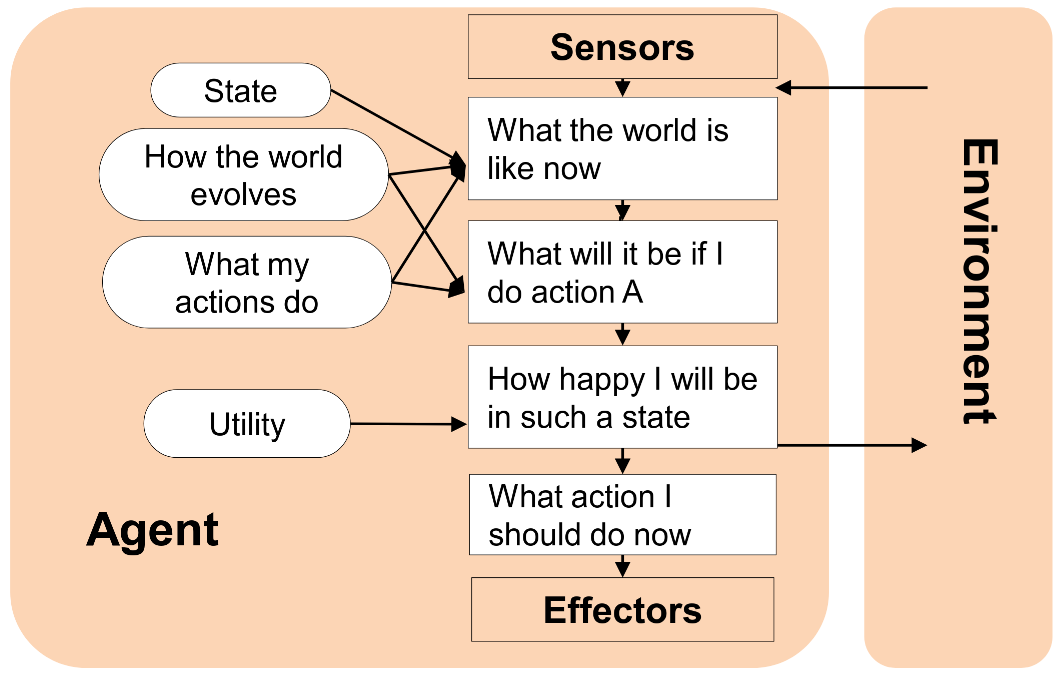
\includegraphics[width=.9\linewidth]{./images/utility-based-agent-diagram.png}
\end{center}

For example, for a driverless taxi:
\begin{itemize}
\item Go to Orchard (destination) via PIE or AYE?
\item Which one charges a lower fare?
\end{itemize}

 \newpage
\subsection{Types of environments}
\label{sec:org47fc3bf}
\begin{itemize}
\item Accessible vs inaccessible: Agent's sensory apparatus gives it access to the complete state of the environment.
\item Deterministic vs nondeterministic: The next state of the environment is completely determined by the current state and the actions selected by the agent.
\item Episodic vs sequential: Each episode is not affected by the previous taken actions.
\item Static vs dynamic: The environment does not change while an agent is deliberating.
\item Discrete vs continuous: A limited number of distinct percepts and actions.
\end{itemize}
\subsubsection{Example: Driverless Taxi}
\label{sec:org8b5d214}
\begin{itemize}
\item Accessible? No. Some traffic information on the road is missing.
\item Deterministic? No. Some cars in front may turn right suddenly.
\item Episodic? No. The current action is based on the previous driving actions.
\item Static? No. When the taxi moves, other cars are moving as well.
\item Discrete? No. Speed, distance and fuel consumption are in real domains.
\end{itemize}
\subsubsection{Example: Chess}
\label{sec:org52706b5}
\begin{itemize}
\item Accessible? Yes. All positions in a chessboard can be observed.
\item Deterministic? Yes. The outcome of each movement can be determined.
\item Episodic? No. The action depends on previous movements.
\item Static? Yes. When there is no clock, when you are considering the next step, your opponent can't move. Semi-static in the case where there is a clock, as you give up the movement once the time is up.
\item Discrete? Yes. All positions and movements are in discrete domains.
\end{itemize}
\subsubsection{Example: Minesweeper}
\label{sec:org7146254}
\begin{itemize}
\item Accessible? No. Mines are hidden.
\item Deterministic? No Mines are randomly assigned in different positions.
\item Episodic? No. The action is based on previous outcomes.
\item Static? Yes. When you are considering the next step, the environment does not change.
\item Discrete? Yes. All positions and movements are in discrete domains.
\end{itemize}
\subsubsection{Example: Slot machines}
\label{sec:org826182f}
\begin{itemize}
\item Accessible? No.
\item Deterministic? No.
\item Episodic? Yes.
\item Static? Yes.
\end{itemize}
\subsection{Design of a problem-solving agent}
\label{sec:orgdc45458}

\subsubsection{Idea}
\label{sec:org6b81bd7}
\begin{itemize}
\item A problem-solving agent systematically considers the expected outcomes of different possible sequences of actions that lead to states of known value.
\item Choose the best one.
\begin{itemize}
\item Shortest journey from A to B?
\item Most cost-effective journey from A to B?
\end{itemize}
\end{itemize}
\subsubsection{Steps}
\label{sec:org80faf48}
\begin{enumerate}
\item Goal formulation
\item Problem formulation
\item Search process
\begin{itemize}
\item Uninformed search for a search without prior knowledge.
\item Informed search for a search with prior knowledge.
\end{itemize}
\item Action execution, which is to follow the recommended route.
\end{enumerate}
\subsubsection{Example: Goal based agent}
\label{sec:org66aa2e2}
\begin{center}
\includegraphics[width=.9\linewidth]{./images/romania-cities-diagram.png}
\end{center}

On a holiday in Romania:
\begin{itemize}
\item Initial state: Currently in Arad. The flight leaves tomorrow from Bucharest.
\item Goal: To be in Bucharest. Other factors include cost, time, most scenic route, etc.
\item State: To be in a city, which is defined by the map above.
\item Action: Transition between states, which are the highways defined by the map.
\end{itemize}
\subsubsection{Example: Vacuum cleaner agent}
\label{sec:orgcab10c4}
\begin{itemize}
\item Robotic vacuum cleaners move autonomously.
\item Some can come back to a docking station to charge their batteries.
\item A few are able to empty their dust containers into the dock as well.
\end{itemize}

 \newpage
\subsubsection{Example: A simple vacuum world}
\label{sec:orgfad5426}
Two locations, each location may or may not contain dirt, and the agent may be in one location or the other.

\begin{center}
\includegraphics[width=.9\linewidth]{./images/simple-vacuum-world-diagram.png}
\end{center}

\begin{itemize}
\item 8 possible world states.
\item Possible actions include turn left, turn right, and suck.
\item The goal is to clean up all dirt. There are two goal states, in the diagram above, 7 and 8.
\end{itemize}

 \newpage
\subsection{Well-defined formulation}
\label{sec:org975048d}

\subsubsection{Definition of a problem}
\label{sec:org3097fbb}
The information used by an agent to decide what to do.
\subsubsection{Specification}
\label{sec:org960f58b}
\begin{itemize}
\item Initial state.
\item Action set, which is all the available actions (successor functions).
\item State space, which is all the states reachable from the initial state.
\begin{itemize}
\item The solution path is a sequence of actions from one state to another.
\end{itemize}
\item Goal test predicate, which can either be a single state, an enumerated list of states, or abstract properties.
\item Cost function, like a path cost \(g(n)\) which is the sum of all action step costs along the path.
\end{itemize}
\subsubsection{Solution}
\label{sec:org7328c7e}
The solution is a path, or a sequence of operators leading from the initial state to a state that satisfies the goal test.
\subsection{Measuring problem-solving performance}
\label{sec:org9b9d3d2}
Search cost:
\begin{itemize}
\item What does it cost to find the solution? How long (time)? How many resources were used (memory)?
\end{itemize}

Total cost of problem-solving:
\begin{itemize}
\item Search cost ("offline", as in when the agent is finding a solution) + execution cost ("online", as in when the agent is executing the solution)
\item Trade-offs are often required. For example, you can either search for a very long time for the optimal solution, or search for a shorter time for a "good enough" solution.
\end{itemize}
\subsubsection{Single-state problem example}
\label{sec:org669acea}
\begin{center}
\includegraphics[width=.9\linewidth]{./images/romania-cities-diagram.png}
\end{center}

\begin{itemize}
\item Initial state: In Arad.
\item Set of possible action and the corresponding next states:
\begin{itemize}
\item Arad \(\rightarrow\) Zerind
\item Arad \(\rightarrow\) Timisoara
\item Arad \(\rightarrow\) Sibiu
\end{itemize}
\item Goal test, which is explicit, like the state being equal to being in Bucharest.
\item Path cost, which is a function. It can be the sum of distances or the number of operators in the executed solution. The executed solution is a sequence of operators leading from the initial state to a goal state.
\end{itemize}
\subsubsection{Example: Vacuum world (single-state version)}
\label{sec:org0b7957c}
\begin{center}
\includegraphics[width=.9\linewidth]{./images/simple-vacuum-world-diagram.png}
\end{center}
\begin{itemize}
\item Initial state: One of the 8 states shown above.
\item Actions: Turn left, turn right, and suck.
\item Goal test: No dirt in any square.
\item Path cost: 1 per action.
\end{itemize}

\begin{center}
\includegraphics[width=.9\linewidth]{./images/simple-vacuum-world-map-of-possible-actions.png}
\end{center}

 \newpage
\subsubsection{Example: 8-puzzle}
\label{sec:org2332684}
\begin{itemize}
\item States: integer locations of tiles.
\begin{itemize}
\item Number of states \(= 9!\)
\end{itemize}
\item Actions: Move blank left, right, up or down.
\item Goal test: Equals to goal state or not, which is shown in the picture below.
\item Path cost: 1 per move.
\end{itemize}

\begin{center}
\includegraphics[width=.9\linewidth]{./images/8-puzzle-start-and-goal-states.png}
\end{center}

 \newpage
\subsubsection{Example: 8-queens}
\label{sec:org7d393f5}
\begin{itemize}
\item States: Any arrangement of 0 to 8 queens on the board.
\item Actions: Add a queen to any empty square.
\item Goal test: 8 queens are on the board, none under attack.
\item Path cost: Not necessary.
\end{itemize}

\begin{center}
\includegraphics[height=20em]{./images/8-queens-puzzle.png}
\end{center}
\subsubsection{Real world problems}
\label{sec:org13809b4}
Route finding problems
\begin{itemize}
\item Routing in computer networks
\item Robot navigation
\item Automated travel advisory
\item Airline travel planning
\end{itemize}

Touring problems:
\begin{itemize}
\item The Travelling salesman problem is a type of shortest tour problem. The goal is to find the shortest path that visits every city exactly once and returns to the origin city.
\end{itemize}

 \newpage
\section{Search algorithms}
\label{sec:org6692025}
\begin{itemize}
\item Search algorithms explore the state space by generating successors of already-explored states.
\item The frontier is the candidate nodes for expansion in the explored set.
\end{itemize}
\subsection{Search strategies}
\label{sec:orge54f1f0}
\begin{itemize}
\item A search strategy is defined by picking the order of node expansion.
\item Strategies are evaluated along the following dimensions:
\begin{itemize}
\item Completeness: Does it always find a solution if one exists?
\item Time complexity: How long does it take to find a solution? This is also the number of nodes generated.
\item Space complexity: The maximum number of nodes in memory.
\item Optimality: Does it always find the best (least-cost) solution?
\end{itemize}
\end{itemize}
\subsubsection{Branching factor}
\label{sec:org504002a}
The branching factor is the maximum number of successors of any node. It is also called the average branching factor.
\subsubsection{Uninformed search}
\label{sec:orgaba991b}
\begin{itemize}
\item Uninformed search strategies use only the information available in the problem definition.
\item Some examples include:
\begin{enumerate}
\item Breadth-first search
\item Uniform-cost search
\item Depth-first search
\item Depth-limited search
\item Iterative deepening search
\end{enumerate}
\end{itemize}
\subsubsection{Informed search}
\label{sec:orge11f01a}
\begin{itemize}
\item Informed search strategies use problem-specific knowledge to guide the search.
\item They are usually more efficient.
\end{itemize}
\subsection{Breadth-first search (BFS)}
\label{sec:orgf6af7d7}
Breadth-first search expands the \textbf{shallowest} unexpanded node, which can be implemented by a first-in-first-out (FIFO) queue.

\begin{center}
\includegraphics[width=.9\linewidth]{./images/breadth-first-search-diagram.png}
\end{center}

Where:
\begin{itemize}
\item \(b\) is the maximum branching factor of the search tree
\item \(d\) is the depth of the least-cost solution
\end{itemize}

The algorithm is complete, and optimal when all step costs are equal.
\subsubsection{Complexity}
\label{sec:org3055aa0}
\begin{itemize}
\item Consider a hypothetical state-space, where every node can be expanded into \(b\) new nodes, with a solution of path-length \(d\).
\item The time complexity would be:
\[1 + b + b^2 + b^3 + \ldots + b^d = O(b^d)\]
\item The space complexity would be the same as the time complexity, as breadth-first search keeps every node in memory, i.e. \(O(b^d)\).
\end{itemize}

\begin{center}
\includegraphics[width=.9\linewidth]{./images/time-and-space-complexity-of-breadth-first-search.png}
\end{center}
\subsection{Uniform-cost search (UCS)}
\label{sec:org27d9b16}
\begin{itemize}
\item Uniform-cost search considers \textbf{edge costs}, and hence expands the unexpanded node with the \textbf{least} path cost \(g\).
\item It is a modification of breadth-first search.
\item Instead of using a first-in-first-out (FIFO) queue, use a priority queue with path cost \(g(n)\) to order the elements.
\item Breadth-first search \(=\) uniform-cost search with \(g(n) = \text{Depth}(n)\)
\end{itemize}

\begin{center}
\includegraphics[width=.9\linewidth]{./images/uniform-cost-search-diagram.png}
\end{center}
\subsubsection{Characteristics}
\label{sec:org977f3e7}
\begin{itemize}
\item Uniform-cost search is complete.
\item The time complexity of uniform-cost search is the number of nodes with the path cost \(g\) that is less than or equal to the cost of the optimal solution. It is equivalent to the number of nodes that pop out from the priority queue.
\item The space complexity of uniform-cost search is the same as the time complexity, i.e. it is the number of nodes with the path cost \(g\) that is less than or equal to the cost of the optimal solution.
\item Uniform-cost search is also optimal.
\end{itemize}

 \newpage
\subsection{Depth-first search (DFS)}
\label{sec:org97e6177}
\begin{itemize}
\item Depth-first search expands the deepest unexpanded node, which can be implemented by using a last-in-first-out (LIFO) stack.
\item It backtracks only when there is no more expansion.
\end{itemize}

\begin{center}
\includegraphics[width=.9\linewidth]{./images/depth-first-search-diagram.png}
\end{center}
\subsubsection{Characteristics}
\label{sec:orgb49b0a5}
Let \(m\) be the maximum depth of the state space.
\begin{itemize}
\item For the characteristic of completeness:
\begin{itemize}
\item Depth-first search is not complete for infinite-depth spaces.
\item It is not complete for finite-depth spaces with loops, but it is complete when these finite-depth spaces with loops have repeated-state checking.
\item It is complete for finite-depth spaces without loops.
\end{itemize}
\item The time complexity of depth-first search is \(O(b^m)\). If the solutions are dense, depth-first search may be much faster than breath-first search.
\item The space complexity of depth-first search is \(O(bm)\).
\item Depth-first search is not optimal.
\end{itemize}

 \newpage
\subsubsection{Depth-limited search}
\label{sec:org2c394df}
\begin{itemize}
\item Depth-limited search is a depth-first search with a \textbf{cut-off} on the maximum depth (\(I\)) of a path to avoid infinite searching.
\item It is complete, if the maximum depth (\(I\)) is greater or equal to the depth of the least cost solution.
\item The time complexity of depth-limited search is \(O(b^l)\).
\item The space complexity of depth-limited search is \(O(bl)\).
\item Depth-limited search is not optimal.
\end{itemize}

 \newpage
\subsection{Iterative deepening search}
\label{sec:orgb6d62f3}
Iterative deepening search iteratively estimates the maximum depth \(I\) of a depth-limited search one by one.
\subsubsection{Limit is 0}
\label{sec:orgbec35ea}
\begin{center}
\includegraphics[width=.9\linewidth]{./images/iterative-deepening-search-limit-is-zero.png}
\end{center}
\subsubsection{Limit is 1}
\label{sec:orgdc2d7a6}
\begin{center}
\includegraphics[width=.9\linewidth]{./images/iterative-deepening-search-limit-is-one.png}
\end{center}
\subsubsection{Limit is 2}
\label{sec:org2a1c1ae}
\begin{center}
\includegraphics[width=.9\linewidth]{./images/iterative-deepening-search-limit-is-two.png}
\end{center}
\subsubsection{Limit is 3}
\label{sec:org5d4517c}
\begin{center}
\includegraphics[width=.9\linewidth]{./images/iterative-deepening-search-limit-is-three.png}
\end{center}
\subsubsection{Pseudocode implementation}
\label{sec:org2b7b0bd}
\begin{minted}[]{lua}
function interative_deepening_search(problem) returns a solution sequence
    inputs: problems, a problem

    for depth = 0 to infinity do
        if depth_limited_search(problem, depth) succeeds then return its result end
    end
end
\end{minted}
\subsubsection{Characteristics}
\label{sec:org5fd6a72}
\begin{itemize}
\item The iterative deepening search is complete.
\item The time complexity of the iterative deepening search is \(O(b^d)\).
\item The space complexity of the iterative deepening search is \(O(bd)\).
\item Iterative deepening search is optimal.
\end{itemize}
\subsection{Summary of search algorithms}
\label{sec:org86fd6ac}
\begin{center}
\begin{tabular}{|m{5em}|m{4em}|m{4em}|m{4em}|m{4em}|m{5em}|m{6em}|}
\hline
Criterion & Breadth-first & Uniform-cost & Depth-first & Depth-limited & Iterative deepening & Bidirectional (if applicable)\\
\hline
Time & \(b^d\) & \(b^d\) & \(b^m\) & \(b^l\) & \(b^d\) & \(b^{\frac{d}{2}}\)\\
\hline
Space & \(b^d\) & \(b^d\) & \(bm\) & \(bl\) & \(bd\) & \(b^{\frac{d}{2}}\)\\
\hline
Optimal & Yes & Yes & No & No & Yes & Yes\\
\hline
Complete & Yes & Yes & No & Yes, if \(l \ge d\) & Yes & Yes\\
\hline
\end{tabular}
\end{center}

 \newpage
\subsection{General search}
\label{sec:org10ffad5}

\subsubsection{Uninformed search strategies}
\label{sec:orgf8f9e67}
\begin{itemize}
\item \textbf{Systematic} generation of new states to pass the goal test
\item \textbf{Inefficient}, as it has exponential space and time complexity.
\end{itemize}
\subsubsection{Informed search strategies}
\label{sec:org4cc9667}
\begin{itemize}
\item Uses \textbf{problem-specific} knowledge to decide the order or node expansion.
\item For example, the best-first search expands the most desirable unexpanded node.
It makes use of an \textbf{evaluation function} to \textbf{estimate} the \textbf{"desirability"} of each node.
\end{itemize}
\subsection{Evaluation function}
\label{sec:org4f62151}
\begin{itemize}
\item The path-cost function \(g(n)\) is the cost from the initial state to the current state (search node) \(n\). It does not provide any information on the cost \textbf{towards the goal}.
\item The evaluation function needs to estimate costs to the closest goal.
\item The "heuristic" function \(h(n)\) is the estimated cost of the cheapest path from \(n\) to a goal state \(h(n)\).
\begin{itemize}
\item The exact cost cannot be determined.
\item The function depends only on the state at that node.
\item \(h(n)\) is not larger than the real cost.
\end{itemize}
\end{itemize}
\subsection{Greedy search}
\label{sec:org71a1e94}
\begin{itemize}
\item Greedy search expands the node that \textbf{appears} to be closest to the goal.
\item The evaluation function \(h(n)\) estimates the cost from \(n\) to the \textbf{goal}.
\end{itemize}
\subsubsection{Pseudocode implementation}
\label{sec:orgeae118a}
\begin{minted}[]{lua}
function greedy_search(problem) returns solution
    return best_first_search(problem, h)    -- h (goal) = 0
end
\end{minted}
\subsubsection{Example}
\label{sec:org9125c4f}
\(h(n)\) is the straight-line distance from \(n\) to \textbf{Bucharest}.

\begin{center}
\includegraphics[height=15em]{./images/greedy-search-example-diagram.png}
\end{center}

Straight-line distance to Bucharest:
\begin{center}
\begin{tabular}{lr}
Arad & 366\\
Bucharest & 0\\
Craiova & 160\\
Dobreta & 242\\
Efoire & 161\\
Fagaras & 176\\
Giurgiu & 77\\
Hirsova & 151\\
Lasi & 226\\
Lugoj & 244\\
Mehadia & 241\\
Neamt & 234\\
Oradea & 380\\
Pitesti & 98\\
Rimnicu Vilcea & 193\\
Sibiu & 253\\
Timisoara & 329\\
Urziceni & 80\\
Vaslui & 199\\
Zerind & 374\\
\end{tabular}
\end{center}

The heuristic of the straight-line distance to Bucharest is useful, but potentially fallible. Heuristic functions are problem-specific as well.

\begin{enumerate}
\item Initial state:
\begin{center}
\includegraphics[height=15em]{./images/greedy-search-example-initial-state-diagram.png}
\end{center}
\item After expanding Arad:
\begin{center}
\includegraphics[width=.9\linewidth]{./images/greedy-search-example-after-expanding-arad-diagram.png}
\end{center}
\item After expanding Sibiu:
\begin{center}
\includegraphics[width=.9\linewidth]{./images/greedy-search-example-after-expanding-sibiu-diagram.png}
\end{center}
\item After expanding Fagaras:
\begin{center}
\includegraphics[width=.9\linewidth]{./images/greedy-search-example-after-expanding-fagaras-diagram.png}
\end{center}
\end{enumerate}
\subsubsection{Characteristics}
\label{sec:orgb11d292}
Let \(m\) be the maximum depth of the search space.
\begin{itemize}
\item The greedy search algorithm is not complete.
\item The time complexity of greedy search is \(O(b^m)\).
\item The space complexity of greedy search is \(O(b^m)\) as it keeps all nodes in memory.
\item The greedy search algorithm is not optimal.
\end{itemize}

 \newpage
\subsection{A* search}
\label{sec:org28f7515}
\begin{itemize}
\item Uniform-cost search
\begin{itemize}
\item \(g(n)\) is the cost to reach \(n\) (past experience).
\item It is optimal and complete, but can be very inefficient.
\end{itemize}
\item Greedy search
\begin{itemize}
\item \(h(n)\) is the cost from \(n\) to the goal (future prediction).
\item It is neither optimal nor complete, but it cuts search space considerably.
\end{itemize}
\item A* search combines greedy search with uniform-cost search.
\item Evaluation function:
\[f(n) = g(n) + h(n)\]

\begin{itemize}
\item \(f(n)\) is the estimated \textbf{total} cost of the path through \(n\) to the goal
\item If \(g = 0\), then it becomes a greedy search.
\item If \(h = 0\), then it becomes a uniform-cost search.
\end{itemize}
\end{itemize}
\subsubsection{Pseudocode implementation}
\label{sec:org9c97543}
\begin{minted}[]{lua}
function a_star_search(problem) returns solution
    return best_first_search(problem, g + h)
end
\end{minted}

 \newpage
\subsubsection{Example}
\label{sec:org9f2a291}
Using best-first-search with evaluation function \(g + h\):

\begin{center}
\includegraphics[width=.9\linewidth]{./images/a-star-search-example-first-three-steps-diagram.png}
\end{center}

(d) After expanding Rimnicu Vilcea:
\begin{center}
\includegraphics[width=.9\linewidth]{./images/a-star-search-example-fourth-step-diagram.png}
\end{center}

(e) After expanding Fagaras:
\begin{center}
\includegraphics[width=.9\linewidth]{./images/a-star-search-example-fifth-step-diagram.png}
\end{center}

 \newpage

(f) After expanding Pitesti:
\begin{center}
\includegraphics[width=.9\linewidth]{./images/a-star-search-example-sixth-step-diagram.png}
\end{center}
\subsubsection{Complexity}
\label{sec:orge05451f}
\begin{itemize}
\item The time complexity of A* search is exponential with respect to the length of the solution.
\item The space complexity of A* search is the same as the time complexity, i.e. it is exponential with respect to the length of the solution.
\item However, with a good heuristic, significant savings are still possible compared to uninformed search methods.
\end{itemize}
\subsection{Route finding in Manhattan example}
\label{sec:org0d834ba}

\subsubsection{Greedy search}
\label{sec:orgf6a00c2}
\begin{center}
\includegraphics[width=.9\linewidth]{./images/route-finding-in-manhattan-example-greedy-search.png}
\end{center}
\subsubsection{Uniform-cost search}
\label{sec:org72f8d74}
\begin{center}
\includegraphics[width=.9\linewidth]{./images/route-finding-in-manhattan-example-uniform-cost-search.png}
\end{center}
\subsubsection{A* search}
\label{sec:org7495b24}
\begin{center}
\includegraphics[width=.9\linewidth]{./images/route-finding-in-manhattan-example-a-star-search.png}
\end{center}

 \newpage
\section{Constraint satisfaction}
\label{sec:orgddc6c60}
The goal of a constraint satisfaction is to discover some state that satisfies a given set of constraints. Some examples include:
\begin{itemize}
\item 8-queens problem
\item Crypt arithmetic puzzle
\item Sudoku
\item Minesweeper
\end{itemize}
\subsection{Definitions}
\label{sec:org9f920e0}

\subsubsection{State}
\label{sec:org865d2ec}
A state of the problem is defined by an \textbf{assignment} of values to some or all of the variables.
\subsubsection{Consistent assignment (Legal assignment)}
\label{sec:org63cfe0a}
An assignment that does not violate any constraints.
\subsubsection{Solution}
\label{sec:orge0a628b}
A \textbf{solution} to a constraint satisfaction problem is an assignment that gives every variable a value (\textbf{complete}), and the assignment satisfies all the constraints.
\subsection{Real world problems}
\label{sec:org41ea34c}
\begin{itemize}
\item Assignment problems, such as who teaches what class
\item Timetabling problems, such as which class is offered when and where
\item Hardware configuration
\item Transportation scheduling
\item Factory scheduling
\item Floor-planning
\end{itemize}
\subsection{Constraint satisfaction problem (CSP)}
\label{sec:orgff01b63}
\begin{itemize}
\item The state is defined by the \textbf{variables} \(V_i\) with values from the domain \(D_i\).
\item For the 8-queens example:
\begin{itemize}
\item The variables would be the locations of each of the eight queens.
\item The values would be the squares on the board.
\end{itemize}
\item The goal test is a set of \textbf{constraints} specifying allowable combinations of values for subsets of variables.
\begin{itemize}
\item For the 8-queens example, the goal test would be to have no two queens in the same row, column or diagonal.
\end{itemize}
\end{itemize}
\subsection{Examples}
\label{sec:orgcef78ea}

\subsubsection{Crypt arithmetic puzzle}
\label{sec:org036ba3b}
\begin{center}
\includegraphics[height=15em]{./images/crypt-arithmetic-puzzle-image.png}
\end{center}
\begin{itemize}
\item Variables: \(D, E, M, N, O, R, S, Y\)
\item Domains: \(\{0, 1, 2, 3, 4, 5, 6, 7, 8, 9\}\)
\item Constraints:
\begin{itemize}
\item \(Y = D + E\) or \(Y = D + E - 10\), etc.
\item \(D \ne E, D \neq M, D \ne N\), etc.
\item \(M \ne 0, S \ne 0\). These are unary constraints, which concern the value of a single variable.
\end{itemize}
\end{itemize}
\subsubsection{Minesweeper}
\label{sec:org3e749d6}
\begin{center}
\includegraphics[height=14em]{./images/minesweeper-image.png}
\end{center}
\begin{itemize}
\item Variables: The cells
\item Domains: \(\{0; 1\}\) representing \(\{\text{safe}, \text{mined}\}\)
\item Constraints: Each cell has a number \(m \in \{1, \ldots, 8\}\) indicating the number of mines nearby, so \(m\) is equal to the sum of the value of neighbouring cells.
\end{itemize}
\subsubsection{Map colouring}
\label{sec:orgc07910b}
Colour a map so that no adjacent parts have the same colour.
\begin{center}
\includegraphics[height=14em]{./images/map-colouring-image.png}
\end{center}
\begin{itemize}
\item Variables: Countries \(Ci\)
\item Domains: \(\{\text{Red}, \text{Blue}, \text{Green}\}\)
\item Constraints: \(C1 \ne C2, C1 \ne C5\), etc, which are binary constraints.
\end{itemize}
\subsection{Applying standard search}
\label{sec:org06c5e47}
\begin{itemize}
\item The states are defined by the values assigned so far.
\item The initial state is to have all variables unassigned.
\item The possible actions are to assign a value to an unassigned variable.
\item The goal test is to have all variables assigned while violating none of the constraints.
\item Constraints should be represented explicitly, like \(D \ne E\) for example.
\item Use a function to test for constraint satisfaction.
\end{itemize}
\subsubsection{8-queens example}
\label{sec:orga95b5d6}
\begin{itemize}
\item The row the first and second queen occupies: \(V_1, V_2 \in \{1, 2, 3, 4, 5, 6, 7, 8, 9, 10\}\).
\item No attack constraint for \(V_1\) and \(V_2\):
\[\{<1, 3>, <1, 4>, <1, 5>, \ldots, <2, 4>, <2, 5>, \ldots\}\]
\end{itemize}
\subsubsection{Map colouring example}
\label{sec:orgda59752}
\begin{center}
\includegraphics[width=.9\linewidth]{./images/map-colouring-example-diagram.png}
\end{center}

\begin{itemize}
\item Number of variables: \(n\)
\item Maximum depth of the space: \(n\)
\item Depth of solution state: \(n\) (all variables assigned)
\item Search algorithm: Depth-first search
\end{itemize}
\subsection{Backtracking search}
\label{sec:orgcb6fe88}
\begin{itemize}
\item Backtracking search stops the search when constraints have already been violated.
\item Before generating successors, check for constraint violations.
\item If there are constraint violations, backtrack to try something else.
\end{itemize}

\begin{center}
\includegraphics[width=.9\linewidth]{./images/backtracking-search-diagram.png}
\end{center}
\subsubsection{4-queens example}
\label{sec:org59b4b18}
\begin{center}
\includegraphics[width=.9\linewidth]{./images/4-queens-example.png}
\end{center}
\subsection{Heuristics for constraint satisfaction problems}
\label{sec:orge8a821c}
Plain backtracking is an uninformed algorithm. More intelligent kinds of search take into consideration:
\begin{itemize}
\item Which variable to assign next.
\item What order of the values to try for each variable.
\item Implications of current variable assignments for the other unassigned variables through forward checking and \textbf{constraint propagation}.
\item \textbf{Constraint propagation} is propagating the implications of a constraint on one variable onto other variables.
\end{itemize}
\subsubsection{4-queens example without constraint propagation}
\label{sec:orgc50ef87}
\begin{center}
\includegraphics[width=.9\linewidth]{./images/4-queens-example.png}
\end{center}
\subsubsection{4-queens example with constraint propagation}
\label{sec:org8477111}
\begin{center}
\includegraphics[width=.9\linewidth]{./images/4-queens-example-with-constraint-propagation.png}
\end{center}

 \newpage
\subsubsection{Map colouring example}
\label{sec:org0fb65e0}
Graph representation:
\begin{center}
\includegraphics[width=.9\linewidth]{./images/map-colouring-example-graph-representation.png}
\end{center}

Initial state:
\begin{center}
\includegraphics[width=.9\linewidth]{./images/map-colouring-example-initial-state.png}
\end{center}

Step 1:
\begin{center}
\includegraphics[width=.9\linewidth]{./images/map-colouring-example-step-1.png}
\end{center}

Step 2:
\begin{center}
\includegraphics[width=.9\linewidth]{./images/map-colouring-example-step-2.png}
\end{center}

Step 3:
\begin{center}
\includegraphics[width=.9\linewidth]{./images/map-colouring-example-step-3.png}
\end{center}
\subsection{Most constrained variable}
\label{sec:org7dccfef}
The most constrained variable, or the minimum remaining values (MRV) heuristic, is to reduce the branching factor on future choices by selecting the variable that is involved in the \textbf{largest number of constraints} on unassigned variables.

\begin{center}
\includegraphics[width=.9\linewidth]{./images/most-contrained-variable-map-colouring-example.png}
\end{center}

 \newpage
\subsection{Least constraining value}
\label{sec:orgb5ad572}
The least constraining value heuristic is to choose the value that leaves maximum flexibility for subsequent variable assignments.

\begin{center}
\includegraphics[width=.9\linewidth]{./images/least-constraining-value-map-colouring-example.png}
\end{center}
\subsection{Minimum-conflicts heuristic (8-queens)}
\label{sec:org5add920}
\begin{itemize}
\item The minimum-conflicts heuristic is a local heuristic search method for solving constraint satisfaction problems.
\item Given an initial assignment, select a variable in the scope of a violated constraint and assign it to the value that minimises the number of violated constraints.
\end{itemize}

\begin{center}
\includegraphics[width=.9\linewidth]{./images/minimum-conflicts-heuristic-8-queens-example.png}
\end{center}

 \newpage
\section{Games playing}
\label{sec:org7ae6e0c}

\subsection{Abstraction}
\label{sec:org0faeb94}
\begin{itemize}
\item An abstraction is an ideal representation of real-world problems.
\item Some examples include board games, chess, go, etc., as an abstraction of war games.
\item Abstractions have perfect information, as they are fully observable.
\item An abstraction that is accurately formulated represents the full state space of a problem.
\end{itemize}
\subsection{Uncertainty}
\label{sec:orgfdd9acc}
\begin{itemize}
\item Uncertainty takes into account the existence of hostile agents (players).
\item These agents are acting to diminish the agent's well-being.
\item Uncertainty about the actions of other agents is not due to the effect of non-deterministic actions and not due to randomness.
\item This uncertainty is a contingency problem.
\end{itemize}
\subsection{Complexity}
\label{sec:orge3ef109}
\begin{itemize}
\item Games are abstract but not simple.
\item For example, in chess, the average branching factor is 35, and chess has a game length greater than 50 moves, which makes its complexity \(35^{50}\), or \(10^{40}\) for legal moves.
\item Games are usually time-limited, which means a complete search for the optimal solution is not possible.
\item There is hence uncertainty on the action's desirability, and search efficiency is crucial.
\end{itemize}

 \newpage
\subsection{Types of games}
\label{sec:org48f3687}
Perfect information below refers to each player having complete information about the opponent's position, as well as the choices available to the opponent.

\begin{center}
\begin{tabular}{l|l|l}
Information type & Deterministic & Chance\\
\hline
Perfect information & Chess, Checkers, Go, Othello & Backgammon, Monopoly\\
Imperfect information &  & Bridge, Poker, Scrabble, Nuclear war\\
\end{tabular}
\end{center}
\subsection{Games as a search problem}
\label{sec:orge771316}
\begin{itemize}
\item The initial state is the initial board configuration and an indication of who makes the first move.
\item The operators are the legal moves.
\item The terminal test determines when the game is over.
\item The utility function or the payoff function is a function that returns a numeric score to quantify the outcome of a game.
\begin{itemize}
\item For example, in chess, +1 for a win, -1 for a loss, and 0 for a draw.
\end{itemize}
\end{itemize}

 \newpage
\subsection{Game tree for tic-tac-toe}
\label{sec:org2782e89}
\begin{itemize}
\item The utility value of the terminal state is from the point of view of MAX.
\item MAX uses the search tree to determine the best move.
\end{itemize}

\begin{center}
\includegraphics[width=.9\linewidth]{./images/tic-tac-toe-game-tree.png}
\end{center}

 \newpage
\subsection{Search strategy example}
\label{sec:orgbaba4f5}
\begin{center}
\includegraphics[width=.9\linewidth]{./images/search-strategy-example-diagram-1.png}
\end{center}

\begin{center}
\includegraphics[width=.9\linewidth]{./images/search-strategy-example-diagram-2.png}
\end{center}

 \newpage
\subsection{Minimax search strategy}
\label{sec:orgd53bc3c}
\begin{itemize}
\item A search strategy is defined as finding a sequence of moves that leads to a terminal state or a goal being achieved.
\item Minimax search strategy maximises one's own utility and minimises the opponent's.
\item The assumption of the minimax search strategy is that the opponent does the same.
\end{itemize}
\subsubsection{Process}
\label{sec:org9ab8323}
\begin{enumerate}
\item Generate the entire game tree down to the terminal states.
\item Calculate utility.
\begin{enumerate}
\item Assess the utility of each terminal state.
\item Determine the best utility of the parents of the terminal state.
\item Repeat the process for their parents until the root is reached.
\end{enumerate}
\item Select the best move, which is the move with the highest utility value.
\end{enumerate}

 \newpage
\subsubsection{Perfect decisions}
\label{sec:org6aaac5c}
\begin{itemize}
\item A perfect decision is when no time limit is imposed, so the search algorithm can generate the complete search tree.
\item There are two players, MAX and MIN.
\begin{itemize}
\item Both players will choose moves with the best achievable payoff against the best play by the other player.
\item MAX tries to maximise the utility, assuming that MIN will try to minimise it.
\end{itemize}
\end{itemize}

\begin{center}
\includegraphics[width=.9\linewidth]{./images/minimax-algorithm-perfect-decisions-diagram.png}
\end{center}

 \newpage
\subsubsection{Imperfect decisions}
\label{sec:orgdc758bd}
\begin{itemize}
\item For games like chess with a high branching factor, such as 35, each player typically makes 50 moves.
\item In this case, the complete game tree would need to examine \(35^{100}\) positions.
\item With time and space requirements, a complete game tree search is intractable and hence it is impractical to make perfect decisions.
\item With the above constraints, the minimax algorithm needs to be modified in two ways:
\begin{enumerate}
\item The utility function needs to be replaced by an \textbf{estimated} desirability of the position, called an evaluation function.
\item The full game tree search is replaced by a partial tree search with a depth limit.
\item The terminal test used in the full game tree search is replaced by a cut-off test.
\end{enumerate}
\end{itemize}
\subsubsection{Evaluation functions}
\label{sec:org536038b}
Evaluation functions return an estimate of the expected utility of the game from a given position.

\begin{center}
\includegraphics[width=.9\linewidth]{./images/evaluation-function-chess-example.png}
\end{center}
\subsection{Othello 4}
\label{sec:org3bcaf81}
\begin{center}
\includegraphics[height=10em]{./images/othello-4-diagram.png}
\end{center}
\begin{itemize}
\item A player can place a new piece in a position if there exists at least one straight (horizontal, vertical, or diagonal) occupied line between the new piece and another piece of the same kind, with one or more contiguous pieces from the opponent player between them.
\item After placing the new piece, the pieces from the opponent player will be captured and become the pieces from the same player.
\item The player with the most pieces on the board wins.
\end{itemize}
\subsubsection{Game flow where "X" plays first}
\label{sec:org7b8cf98}
\begin{center}
\includegraphics[width=.9\linewidth]{./images/othello-4-game-flow-x-plays-first.png}
\end{center}
\subsubsection{Game tree}
\label{sec:org1f78fe6}
\begin{center}
\includegraphics[width=.9\linewidth]{./images/othello-4-game-tree.png}
\end{center}

 \newpage
\section{Agent decision-making and reinforcement learning}
\label{sec:orga0b5977}

\subsection{Maximum expected utility}
\label{sec:orge060394}
The expected utility is a function of the utility function and the outcome probabilities, defined as follows:
\[EU (A | E) = \sum_i P (\text{Result}_i (A) | E, \ \text{Do} (A)) U (\text{Result}_i (A))\]

The principle of maximum expected utility states to choose an action with the highest expected utility (\(EU (A | E)\)).
\subsubsection{Example}
\label{sec:orgcc2a168}
For a robot with two options:
\begin{enumerate}
\item Turn right
\begin{itemize}
\item Hits wall (\(P = 0.1, \ U = 0\))
\item Finds target (\(P = 0.9, \ U = 10\))
\end{itemize}
\item Turn left
\begin{itemize}
\item Fall in water (\(P = 0.3, \ U = 0\))
\item Finds target (\(P = 0.7, \ U = 10\))
\end{itemize}
\end{enumerate}

The robot should choose to turn right.

 \newpage
\subsection{Agent-environment interface}
\label{sec:orgda0e21e}
\begin{center}
\includegraphics[width=.9\linewidth]{./images/agent-environment-interface-flow-chart.png}
\end{center}
\begin{itemize}
\item The agent and environment interact at discrete time steps: \(t = 0, 1, 2, \ldots\)
\item It observes state at step \(t: s_t \in S\)
\item It produces action at step \(t: a_t \in A(s_t)\)
\item It gets a resulting reward: \(r_{t + 1} \in \mathbb{R}\)
\item It also gets the resulting next state: \(s_{t + 1}\)
\end{itemize}

\begin{center}
\includegraphics[width=.9\linewidth]{./images/agent-environment-interface-procedure.png}
\end{center}

 \newpage
\subsection{Making complex decisions}
\label{sec:orgfc024f9}
\begin{itemize}
\item Make a sequence of decisions.
\begin{itemize}
\item Agent's utility depends on a sequence of decisions.
\item Sequential decision-making.
\end{itemize}
\item Markov property
\begin{itemize}
\item Transition property depends only on the current state, not on previous history (how that state was reached).
\item Markov decision processes.
\end{itemize}
\end{itemize}
\subsubsection{Markov decision processes}
\label{sec:org3add3c9}
\begin{itemize}
\item Components:
\begin{itemize}
\item Markov \textbf{states} \(s\), beginning with the initial state \(s_0\).
\item \textbf{Actions} \(a\), where each state has actions \(A(s)\) available from it.
\item \textbf{Transition model} \(P (s' | s, a)\), where the assumption is that the probability of going from \(s'\) from \(s\) depends only on \(s\) and \(a\) and not on any other past actions or states.
\item \textbf{Reward function} \(R(s)\).
\end{itemize}
\item \textbf{Policy} \(\pi (s)\), which is the action that an agent takes in any given state. This is the "solution" to a Markov decision process.
\end{itemize}

 \newpage
\subsection{Game show}
\label{sec:org6484961}
\begin{itemize}
\item A series of questions with increasing levels of difficulty and payoff.
\item At each step, take your earnings and quit, or go for the next question. If you answer wrong, you lose everything.
\end{itemize}

\begin{center}
\includegraphics[width=.9\linewidth]{./images/game-show-flow-chart.png}
\end{center}

\begin{itemize}
\item The probability of guessing correctly is 0.1.
\item Expected payoff for continuing is \(0.1 \times 61,100 + 0.9 \times 0 = 6,110\).
\item The optimal decision would be to quit.
\item In question 3:
\begin{itemize}
\item Payoff for quitting: \$1,100
\item Payoff for continuing: \(0.5 \times 11,100 = 5,550\)
\end{itemize}
\item In question 2:
\begin{itemize}
\item \$100 for quitting versus \$4,162 for continuing.
\end{itemize}
\item In question 1:
\begin{itemize}
\item \$0 for quitting versus \$100 for continuing.
\end{itemize}
\end{itemize}

 \newpage
\subsection{Grid world}
\label{sec:orge1034c0}
\begin{center}
\includegraphics[height=10em]{./images/grid-world-image.png}
\end{center}

\begin{center}
\includegraphics[height=10em]{./images/grid-world-policy-image.png}
\end{center}

\begin{center}
\includegraphics[height=13em]{./images/grid-world-diagram.png}
\end{center}

\begin{center}
\includegraphics[height=13em]{./images/grid-world-policy-diagram.png}
\end{center}

 \newpage
\subsection{Solving Markov decision processes (MDPs)}
\label{sec:orgde4e1e2}
\begin{itemize}
\item MDP components:
\begin{itemize}
\item \textbf{States} \(s\)
\item \textbf{Actions} \(a\)
\item \textbf{Transition model} \(P (s' | s, a)\)
\item \textbf{Reward function} \(R (s)\)
\end{itemize}
\item The solution:
\begin{itemize}
\item \textbf{Policy} \(\pi (s)\): mapping from states to actions
\end{itemize}
\end{itemize}
\subsubsection{Maximising expected utility}
\label{sec:org6c2bce3}
\begin{itemize}
\item The optimal policy should maximise the expected utility over all possible state sequences produced by following that policy:
\[\sum_{\text{State sequences starting from } s_0} P (\text{sequence}) U (\text{sequence})\]
\item The utility of a state sequence is the sum of rewards of individual states.
\item However, there is an issue with infinite state sequences.
\end{itemize}
\subsubsection{Utility of state sequences}
\label{sec:org1c79ada}
\begin{itemize}
\item Usually, the utility of a state sequence is the sum of the rewards of the individual state.
\item However, due to the infinite state sequences problem, each of the rewards of the individual states has to be discounted by a factor \(\gamma\) between 0 and 1.
\begin{align*}
U([s_0, s_1, s_2, \ldots]) &= R(s_0) + \gamma R (s_1) + \gamma^2 R(s_2) + \ldots \\
&= \sum_{t = 0}^{\infty} \gamma^t R(s_t) \le \frac{R_{max}}{1 - \gamma} \quad (0 < \gamma < 1)
\end{align*}
\begin{itemize}
\item Sooner rewards count more than later rewards.
\item This makes sure the total utility stays bounded.
\item It helps algorithms converge.
\end{itemize}
\end{itemize}
\subsubsection{Utility of states}
\label{sec:org58bb948}
\begin{itemize}
\item Expected utility obtained by policy \(\pi\) starting in state \(s\) is:
\[U^{\pi} (s) = \sum_{\text{State sequences starting from } s} P (\text{sequence}) U (\text{sequence})\]
\item The "true" utility of a state, denoted \(U(s)\), is the expected sum of discounted rewards if the agent executes an optimal policy starting in state \(s\).
\item This is reminiscent of the minimax values of states.
\end{itemize}
\subsubsection{Finding the utilities of states}
\label{sec:org4f6bd60}
\begin{center}
\includegraphics[height=18em]{./images/finding-the-utilities-of-state-tree.png}
\end{center}
\begin{itemize}
\item The expected utility of taking action \(a\) in state \(s\) is:
\[\sum_{s'} P (s' | s, a) U (s')\]
\item The optimal action is given by:
\[\pi^{*} (s) = \underset{a \in A(s)}{\arg \max} \sum_{s'} P (s' | s, a) U(s')\]
\item The recursive expression for \(U(s)\) in terms of the utilities of its successor states is:
\[U(s) = R(s) + \gamma \max_a \sum_{s'} P (s' | s, a) U (s')\]
\end{itemize}
\subsection{Bellman equation}
\label{sec:org7e92e4a}
\begin{center}
\includegraphics[height=20em]{./images/bellman-equation-tree.png}
\end{center}
\begin{itemize}
\item The recursive relationship between the utilities of successive states:
\[U (s) = R(s) + \gamma \underset{a \in A(s)}{\max} \sum_{s'} P (s' | s, a) U(s')\]
\item For \(N\) states, we get \(N\) equations in \(N\) unknowns.
\begin{itemize}
\item Solving them solves the Markov decision process.
\item Trying to solve them using expectimax search would run into issues with infinite sequences.
\item Instead, they should be solved algebraically.
\item There are two methods to doing so, \textbf{value iteration} and \textbf{policy iteration}.
\end{itemize}
\end{itemize}

 \newpage
\subsubsection{Value iteration}
\label{sec:org62e6c60}
\begin{itemize}
\item Start out with every \(U(s) = 0\).
\item Iterate until convergence.
\begin{itemize}
\item During the \(i\)-th iteration, update the utility of each state according to the rule below:
\[U_{i + 1} (s) \leftarrow R(s) + \gamma \underset{a \in A(s)}{\max} \sum_{s'} P(s' | s, a) U_i (s')\]
\end{itemize}
\item In the limit of infinitely many iterations, the correct utility values are guaranteed to be found.
\item In practice, however, there is no need to use an infinite number of iterations.
\end{itemize}
\subsubsection{Policy iteration}
\label{sec:orgb2ebd11}
\begin{itemize}
\item Start with some initial policy \(\pi_0\) and alternate between the following steps:
\begin{itemize}
\item \textbf{Policy evaluation}: Calculate \(U^{\pi_i} (s)\) for every state \(s\).
\item \textbf{Policy improvement}: Calculate a new policy \(\pi_{i + 1}\) based on the updated utilities.
\[\pi^{i + 1} (s) = \underset{a \in A(s)} {\arg \max} \sum_{s'} P (s' | s, a) U^{\pi_i} (s')\]
\end{itemize}
\end{itemize}
\subsection{Temporal difference prediction}
\label{sec:org7d00b13}
\begin{itemize}
\item Policy evaluation (the prediction problem):
\begin{itemize}
\item For a given policy \(p\), compute the state-value function \(V^{\pi}\).
\item The simplest temporal difference method, \(TD(0)\):
\[V(s_t) \leftarrow v(s_t) + \alpha [\underbrace{r_{t + 1} + \gamma V(s_{t + 1})}_{\text{Target: an estimate of the return}} - V(s_t)]\]
\end{itemize}
\end{itemize}
\subsubsection{Simplest temporal difference method}
\label{sec:orgeac0377}
\[V(s_t) \leftarrow v(s_t) + \alpha [r_{t + 1} + \gamma V(s_{t + 1}) - V(s_t)]\]

\begin{center}
\includegraphics[width=.9\linewidth]{./images/simplest-temporaral-difference-method-tree.png}
\end{center}
\subsubsection{Advantages of temporal difference learning}
\label{sec:org24bc3dc}
\begin{itemize}
\item Temporal difference methods do not require a model of the environment, only experience.
\item Temporal difference methods can be fully incremental.
\begin{itemize}
\item The model can learn \textbf{before} knowing the final outcome, which results in less memory used and lower peak computation.
\item The model can learn \textbf{without} the final outcome, which means it can learn from incomplete sequences.
\end{itemize}
\end{itemize}

 \newpage
\section{Python reference}
\label{sec:orge8021e6}

\subsection{Default imports}
\label{sec:orga36bb3c}
\begin{minted}[]{python}
import numpy as np
import pandas as pd
import matplotlib.pyplot as plt
import seaborn as sb

# Set the theme for seaborn
sb.set_theme()
\end{minted}
\subsection{\href{https://pandas.pydata.org/docs/reference/api/pandas.read\_csv.html}{Loading the data}}
\label{sec:org21e047a}
\begin{minted}[]{python}
data = pd.read_csv("./data.csv")
print(data.shape)
\end{minted}

\phantomsection
\label{org8cec87b}
\begin{verbatim}
(1460, 81)
\end{verbatim}


 \newpage
\subsection{\href{https://pandas.pydata.org/docs/reference/api/pandas.DataFrame.select\_dtypes.html}{Selecting all variables of a type}}
\label{sec:orge3edcec}
\begin{minted}[]{python}
numeric_data = data.select_dtypes("number")
print(numeric_data.shape)
\end{minted}

\phantomsection
\label{org2ddf84f}
\begin{verbatim}
(1460, 38)
\end{verbatim}


Get the actual numeric data from the data description.
\begin{minted}[]{python}
numeric_variables = [
    "LotArea",
    "GrLivArea",
    "TotalBsmtSF",
    "GarageArea",
    "SalePrice"
]
numeric_data = data[numeric_variables]
print(numeric_data.head())
\end{minted}

\phantomsection
\label{orgf8c8645}
\begin{verbatim}
   LotArea  GrLivArea  TotalBsmtSF  GarageArea  SalePrice
0     8450       1710          856         548     208500
1     9600       1262         1262         460     181500
2    11250       1786          920         608     223500
3     9550       1717          756         642     140000
4    14260       2198         1145         836     250000
\end{verbatim}
\subsection{\href{https://pandas.pydata.org/docs/reference/api/pandas.DataFrame.head.html}{Head of the data}}
\label{sec:orgf5d4540}
\begin{minted}[]{python}
print(numeric_data.head())
\end{minted}

\phantomsection
\label{org6e35c4e}
\begin{verbatim}
   LotArea  GrLivArea  TotalBsmtSF  GarageArea  SalePrice
0     8450       1710          856         548     208500
1     9600       1262         1262         460     181500
2    11250       1786          920         608     223500
3     9550       1717          756         642     140000
4    14260       2198         1145         836     250000
\end{verbatim}
\subsection{\href{https://pandas.pydata.org/docs/reference/api/pandas.DataFrame.describe.html}{Statistical description of the data}}
\label{sec:org8f114ac}
\begin{minted}[]{python}
print(numeric_data.describe())
\end{minted}

\phantomsection
\label{org3ef427d}
\begin{verbatim}
             LotArea    GrLivArea  TotalBsmtSF   GarageArea      SalePrice
count    1460.000000  1460.000000  1460.000000  1460.000000    1460.000000
mean    10516.828082  1515.463699  1057.429452   472.980137  180921.195890
std      9981.264932   525.480383   438.705324   213.804841   79442.502883
min      1300.000000   334.000000     0.000000     0.000000   34900.000000
25%      7553.500000  1129.500000   795.750000   334.500000  129975.000000
50%      9478.500000  1464.000000   991.500000   480.000000  163000.000000
75%     11601.500000  1776.750000  1298.250000   576.000000  214000.000000
max    215245.000000  5642.000000  6110.000000  1418.000000  755000.000000
\end{verbatim}
\subsection{\href{https://pandas.pydata.org/docs/reference/api/pandas.DataFrame.skew.html}{Skew of the data}}
\label{sec:org59c7e63}
\begin{minted}[]{python}
print(numeric_data.skew())
\end{minted}

\phantomsection
\label{org9fcd802}
\begin{verbatim}
LotArea        12.207688
GrLivArea       1.366560
TotalBsmtSF     1.524255
GarageArea      0.179981
SalePrice       1.882876
dtype: float64
\end{verbatim}


 \newpage
\subsection{Getting the number of outliers}
\label{sec:orgebb755e}
\begin{minted}[]{python}
quartile_1 = numeric_data.quantile(0.25)
quartile_3 = numeric_data.quantile(0.75)
interquartile_range = quartile_3 - quartile_1

number_of_outliers = (
    (numeric_data < quartile_1 - 1.5 * interquartile_range)
    | (numeric_data > quartile_3 + 1.5 * interquartile_range)
).sum()

print("Number of outliers:")
print(number_of_outliers)
\end{minted}

\phantomsection
\label{org1e0a979}
\begin{verbatim}
Number of outliers:
LotArea        69
GrLivArea      31
TotalBsmtSF    61
GarageArea     21
SalePrice      61
dtype: int64
\end{verbatim}
\subsection{\href{https://pandas.pydata.org/docs/reference/api/pandas.DataFrame.corr.html}{Correlation matrix}}
\label{sec:org5dd0c85}
\begin{minted}[]{python}
print(numeric_data.corr())
\end{minted}

\phantomsection
\label{orge6a94f8}
\begin{verbatim}
              LotArea  GrLivArea  TotalBsmtSF  GarageArea  SalePrice
LotArea      1.000000   0.263116     0.260833    0.180403   0.263843
GrLivArea    0.263116   1.000000     0.454868    0.468997   0.708624
TotalBsmtSF  0.260833   0.454868     1.000000    0.486665   0.613581
GarageArea   0.180403   0.468997     0.486665    1.000000   0.623431
SalePrice    0.263843   0.708624     0.613581    0.623431   1.000000
\end{verbatim}


 \newpage
\subsection{\href{https://pandas.pydata.org/docs/reference/api/pandas.DataFrame.astype.html}{Converting data types}}
\label{sec:org91a18e6}
\begin{minted}[]{python}
categorical_variables = [
    "MSSubClass",
    "Neighborhood",
    "BldgType",
    "OverallQual",
]

categorical_data = data[categorical_variables]
print("Data types:")
print(categorical_data.dtypes)
print()

categorical_data = categorical_data.astype("category")
print("Data types:")
print(categorical_data.dtypes)
\end{minted}

\phantomsection
\label{org5684155}
\begin{verbatim}
Data types:
MSSubClass       int64
Neighborhood    object
BldgType        object
OverallQual      int64
dtype: object

Data types:
MSSubClass      category
Neighborhood    category
BldgType        category
OverallQual     category
dtype: object
\end{verbatim}

 \newpage
\subsection{\href{https://pandas.pydata.org/docs/reference/api/pandas.DataFrame.groupby.html}{Grouping data}}
\label{sec:org53edd45}
\begin{minted}[]{python}
# Need to call ".size" on the grouped data
# to actually group the data.
grouped_data = data.groupby(
    by=["OverallQual", "BldgType"],

    # Get rid of the deprecation warning
    observed=False,
).size()

# Unstack the data so there is a 2D array
# that is plottable.
grouped_data = grouped_data.unstack()

print(grouped_data.head())
\end{minted}

\phantomsection
\label{orge1b989d}
\begin{verbatim}
BldgType      1Fam  2fmCon  Duplex  Twnhs  TwnhsE
OverallQual                                      
1              2.0     NaN     NaN    NaN     NaN
2              3.0     NaN     NaN    NaN     NaN
3             16.0     1.0     3.0    NaN     NaN
4             90.0     8.0     8.0    6.0     4.0
5            339.0    15.0    31.0    3.0     9.0
\end{verbatim}


\begin{verbatim}
BldgType      1Fam  2fmCon  Duplex  Twnhs  TwnhsE
OverallQual
1              2.0     NaN     NaN    NaN     NaN
2              3.0     NaN     NaN    NaN     NaN
3             16.0     1.0     3.0    NaN     NaN
4             90.0     8.0     8.0    6.0     4.0
5            339.0    15.0    31.0    3.0     9.0
\end{verbatim}


 \newpage
\subsection{\href{https://scikit-learn.org/stable/modules/generated/sklearn.model\_selection.train\_test\_split.html}{Splitting data randomly}}
\label{sec:org7ec34db}
The code below imports the \texttt{train\_test\_split} function and splits the data set into 70\% training data and 30\% test data.
\begin{minted}[]{python}
from sklearn.model_selection import train_test_split
training_data, test_data = train_test_split(data, test_size=0.3)
print(training_data.shape)
print(test_data.shape)
\end{minted}

\phantomsection
\label{orgd667174}
\begin{verbatim}
(1022, 81)
(438, 81)
\end{verbatim}
\subsection{\href{https://scikit-learn.org/stable/modules/generated/sklearn.linear\_model.LinearRegression.html}{Linear regression}}
\label{sec:org4649b56}
\begin{minted}[]{python}
from sklearn.linear_model import LinearRegression
model = LinearRegression()
\end{minted}
\subsubsection{Training the model}
\label{sec:orgdac5f3a}
\begin{minted}[]{python}
training_data_x = pd.DataFrame(training_data["GrLivArea"])
training_data_y = pd.DataFrame(training_data["SalePrice"])
model.fit(training_data_x, training_data_y)
\end{minted}
\subsubsection{Scoring the model}
\label{sec:org1c4a97d}
\begin{minted}[]{python}
accuracy = model.score(training_data_x, training_data_y)
print(accuracy)
\end{minted}

\phantomsection
\label{org44b2f79}
\begin{verbatim}
0.518488052675584
\end{verbatim}
\subsubsection{Predicting data}
\label{sec:org3024c58}
\begin{minted}[]{python}
prediction = model.predict(training_data_x)
print(prediction)
\end{minted}

\phantomsection
\label{orgd60c157}
\begin{verbatim}
[[112899.37012923]
 [177936.06711062]
 [246798.45214974]
 ...
 [205391.00493668]
 [232170.82134078]
 [227444.97138711]]
\end{verbatim}
\subsubsection{Getting the model coefficients after training}
\label{sec:org3a5e54d}
\begin{minted}[]{python}
model_coefficients = model.coef_[0][0]
print(model_coefficients)
\end{minted}

\phantomsection
\label{org0617a02}
\begin{verbatim}
112.5202369920301
\end{verbatim}
\subsubsection{Forming the equation of the line}
\label{sec:org3c526c8}
\begin{minted}[]{python}
regression_x = training_data_x
regression_y = model_coefficients * regression_x + model.intercept_
print(regression_x.head())
print()
print(regression_y.head())
\end{minted}

\phantomsection
\label{orgff38f29}
\begin{verbatim}
      GrLivArea
1215        894
1018       1472
787        2084
309        1944
988        2030

          GrLivArea
1215  112899.370129
1018  177936.067111
787   246798.452150
309   231045.618971
988   240722.359352
\end{verbatim}

 \newpage
\subsubsection{Plotting the graph}
\label{sec:orgf3e225a}
\begin{minted}[]{python}
plt.figure(figsize=(16, 8))
plt.scatter(training_data_x, training_data_y)
plt.plot(regression_x, regression_y, "r-", linewidth=3)
\end{minted}

\begin{center}
\includegraphics[width=.9\linewidth]{./.ob-jupyter/9d5f8d566c994d646bf055061033c499a52025d1.png}
\label{org8c10660}
\end{center}
\subsection{\href{https://scikit-learn.org/stable/modules/generated/sklearn.cluster.KMeans.html}{K-means clustering}}
\label{sec:org4d2104f}
The number of clusters should be guessed based on the data.
\begin{minted}[]{python}
from sklearn.cluster import KMeans
model = KMeans(n_clusters=4)
\end{minted}
\subsubsection{Training the model}
\label{sec:orgc82b112}
\begin{minted}[]{python}
extracted_data = data[["GrLivArea", "GarageArea"]]
model.fit(extracted_data)
\end{minted}
\subsubsection{Getting the cluster centres}
\label{sec:org4a9b915}
\begin{minted}[]{python}
print(pd.DataFrame(model.cluster_centers_))
\end{minted}

\phantomsection
\label{org4348bcd}
\begin{verbatim}
             0           1
0  1557.328479  490.318770
1  2147.264925  625.462687
2  3178.974359  707.717949
3  1029.347664  359.456075
\end{verbatim}
\subsubsection{Predicting the clusters for the data}
\label{sec:org2671b66}
\begin{minted}[]{python}
predicted_clusters = model.predict(extracted_data)
print(pd.DataFrame(predicted_clusters).head())
\end{minted}

\phantomsection
\label{org075b61c}
\begin{verbatim}
   0
0  0
1  3
2  0
3  0
4  1
\end{verbatim}
\subsubsection{Adding the predicted clusters to the data}
\label{sec:org12e4d1c}
\begin{minted}[]{python}
clustered_data = extracted_data.copy()
clustered_data["Cluster"] = pd.Categorical(predicted_clusters)
print(clustered_data.head())
\end{minted}

\phantomsection
\label{org6ab8ff0}
\begin{verbatim}
   GrLivArea  GarageArea Cluster
0       1710         548       0
1       1262         460       3
2       1786         608       0
3       1717         642       0
4       2198         836       1
\end{verbatim}


 \newpage
\subsubsection{Visualising the clusters in a scatter plot}
\label{sec:org9334ebb}
You can view all the possible colour palettes \href{https://seaborn.pydata.org/tutorial/color\_palettes.html\#qualitative-color-palettes}{here}.
\begin{minted}[]{python}
plt.subplots(figsize=(16, 8))
plt.scatter(
    x="GrLivArea",
    y="GarageArea",

    # Colour the points
    # based on the cluster
    c="Cluster",

    # Set a colour map
    cmap="viridis",
    data=clustered_data,
)
\end{minted}

\begin{center}
\includegraphics[width=.9\linewidth]{./.ob-jupyter/87750eed32b3e27ef9698b1b40a8271360d279e8.png}
\label{org9551c15}
\end{center}

 \newpage
\subsubsection{Getting the ideal number of clusters}
\label{sec:orgea99fce}
First, we create a function to calculate the square of the Euclidean distance of one point away from another point.
\begin{minted}[]{python}
def get_squared_euclidean_distance(
    point_1: np.ndarray,
    point_2: np.ndarray,
) -> float:
    """
    A function to get the square of the Euclidean distance between two points.

    The first point and the second point must have the
    same dimensions, i.e. if point_1 is 2 dimensional, with coordinates (x_1, y_1),
    then point_2 should also be 2 dimensional, with coordinates (x_2, y_2).
    """

    # Initialise the squared Euclidean distance
    squared_euclidean_distance = 0

    # Iterate over the coordinates
    for index, point_1_coordinate in enumerate(point_1):

        # Get the coordinate for the second point
        point_2_coordinate = point_2[index]

        # Subtract the coordinates of point 1
        # from the coordinates of point 2,
        # and square the result
        coordinate_euclidean_distance = (
            point_2_coordinate - point_1_coordinate
        ) ** 2

        # Add the Euclidean distance for the coordinate
        # to the squared Euclidean distance
        squared_euclidean_distance += coordinate_euclidean_distance

    # Return the squared Euclidean distance
    return squared_euclidean_distance
\end{minted}

 \newpage

Next, we iterate over the possible number of clusters and fit the k-Means algorithm, while calculating the within-cluster sum of squares.
\begin{minted}[]{python}
# The possible number of clusters
possible_number_of_clusters = list(range(1, 21))

# Initialise the list of the within-cluster sum of squares (WSS)
within_cluster_sum_of_squares_list = []

# Iterate over the number of clusters
for number_of_clusters in possible_number_of_clusters:

    # Initialise the K means clustering model with
    # the number of clusters and fit the model to the data
    model = KMeans(n_clusters=number_of_clusters).fit(extracted_data)

    # Get the centres and predict the clusters for the data
    centres = model.cluster_centers_
    predicted_clusters = model.predict(extracted_data)

    # Initialise the variable to store the within-cluster sum of squares
    within_cluster_sum_of_squares = 0

    # Iterate over the points in the data
    for point_index, point in enumerate(np.array(extracted_data)):

        # Get the centre for the current point
        point_centre = centres[predicted_clusters[point_index]]

        # Calculate the squared Euclidean distance
        squared_euclidean_distance = get_squared_euclidean_distance(
            point_centre, point
        )

        # Add the squared Euclidean distance for the point
        # to the within-cluster sum of squares
        within_cluster_sum_of_squares += squared_euclidean_distance

    # Add the within-cluster sum of squares to the list
    within_cluster_sum_of_squares_list.append(within_cluster_sum_of_squares)
\end{minted}

 \newpage

Lastly, we plot the graph.
\begin{minted}[]{python}
# Plot the graph of within-cluster sum of squares (y)
# against the number of clusters (x)
plt.figure(figsize=(16, 8))
plt.plot(
    possible_number_of_clusters,
    within_cluster_sum_of_squares_list,
)

# Force the x-tick labels to display the number of clusters,
# which are integers, instead of the default
plt.xticks(possible_number_of_clusters)

# Label the x and y axis
plt.xlabel("Number of clusters")
plt.ylabel("Within-cluster sum of squares (WSS)")
\end{minted}

\begin{center}
\includegraphics[width=.9\linewidth]{./.ob-jupyter/d304095916fcd51fb066aca71576b6f61bcbc873.png}
\label{org2c61ccd}
\end{center}

Using the elbow method, we can see that the ideal number of clusters here is 3 clusters.

 \newpage
\subsection{\href{https://scikit-learn.org/stable/modules/generated/sklearn.neighbors.LocalOutlierFactor.html}{Local outlier factor}}
\label{sec:org451fc03}
\begin{itemize}
\item The parameters for the local outlier factor model should be given.
\item The \texttt{contamination} is just the fraction or percentage of outliers.
\end{itemize}
\begin{minted}[]{python}
from sklearn.neighbors import LocalOutlierFactor
model = LocalOutlierFactor(n_neighbors=20, contamination=0.05)
\end{minted}
\subsubsection{Training the model}
\label{sec:org6ba6bb2}
\begin{minted}[]{python}
model.fit(extracted_data)
\end{minted}
\subsubsection{Predicting anomalies}
\label{sec:org6ca04a7}
\begin{minted}[]{python}
labels = model.fit_predict(extracted_data)
print(pd.DataFrame(labels).head())
\end{minted}

\phantomsection
\label{org41c67ab}
\begin{verbatim}
   0
0  1
1  1
2  1
3  1
4  1
\end{verbatim}
\subsubsection{Adding anomalies to the data}
\label{sec:org0aedb30}
\begin{minted}[]{python}
labelled_data = extracted_data.copy()
labelled_data["Anomaly"] = pd.Categorical(labels)
print(labelled_data.head())
\end{minted}

\phantomsection
\label{orga1dbe51}
\begin{verbatim}
   GrLivArea  GarageArea Anomaly
0       1710         548       1
1       1262         460       1
2       1786         608       1
3       1717         642       1
4       2198         836       1
\end{verbatim}
\subsubsection{Visualising the anomalies in the data}
\label{sec:org559d0ad}
You can view all the possible colour palettes \href{https://seaborn.pydata.org/tutorial/color\_palettes.html\#qualitative-color-palettes}{here}.
\begin{minted}[]{python}
plt.subplots(figsize=(16, 8))
plt.scatter(
    x="GrLivArea",
    y="GarageArea",

    # Colour the points
    # based on whether it is
    # an anomaly or not
    c="Anomaly",

    # Set a colour map
    cmap="viridis",
    data=labelled_data
)
\end{minted}

\begin{center}
\includegraphics[width=.9\linewidth]{./.ob-jupyter/a9a37db9ea5cafe166990634044f68a4e93893a4.png}
\label{org0e5b712}
\end{center}
\subsection{\href{https://scikit-learn.org/stable/modules/generated/sklearn.tree.DecisionTreeClassifier.html}{Decision tree}}
\label{sec:org59949b9}
\begin{minted}[]{python}
from sklearn.tree import DecisionTreeClassifier
model = DecisionTreeClassifier(max_depth=2)
\end{minted}
\subsubsection{Training the model}
\label{sec:orgf8554c7}
\begin{minted}[]{python}
training_data_x = pd.DataFrame(training_data["SalePrice"])
training_data_y = pd.DataFrame(training_data["CentralAir"])
model.fit(training_data_x, training_data_y)
\end{minted}
\subsubsection{Scoring the model}
\label{sec:org3479872}
\begin{minted}[]{python}
accuracy = model.score(training_data_x, training_data_y)
print(accuracy)
\end{minted}

\phantomsection
\label{org04673fd}
\begin{verbatim}
0.9500978473581213
\end{verbatim}
\subsubsection{Predicting data}
\label{sec:org29934d7}
\begin{minted}[]{python}
prediction = model.predict(training_data_x)
print(prediction)
\end{minted}

\phantomsection
\label{org6d1be31}
\begin{verbatim}
['Y' 'Y' 'Y' ... 'Y' 'Y' 'Y']
\end{verbatim}


 \newpage
\subsubsection{Plotting the decision tree}
\label{sec:orgcc80d72}
\begin{minted}[]{python}
from sklearn.tree import plot_tree
plt.figure(figsize=(8, 8))
plot_tree(
    model,
    filled=True,
    rounded=True,
    feature_names=["SalePrice"]
)
\end{minted}

\begin{center}
\includegraphics[width=.9\linewidth]{./.ob-jupyter/411a41a2fee2287ec072856fd167b829da235923.png}
\label{org904fe48}
\end{center}

 \newpage
\subsection{\href{https://scikit-learn.org/stable/modules/generated/sklearn.metrics.confusion\_matrix.html}{Confusion matrix}}
\label{sec:org9258f5c}
\begin{minted}[]{python}
from sklearn.metrics import confusion_matrix
matrix = confusion_matrix(training_data_y, prediction)
print(matrix)
\end{minted}

\phantomsection
\label{orgaea97b1}
\begin{verbatim}
[[ 10  51]
 [  0 961]]
\end{verbatim}
\subsubsection{Plotting the confusion matrix}
\label{sec:org2ace095}
\begin{minted}[]{python}
plt.figure(figsize=(8, 8))
sb.heatmap(
    matrix,

    # Annotate the squares
    # in the heatmap
    annot=True,

    # Round the values to 2 decimal places
    fmt=".2f",

    # Set the size of the
    # annotations to 18
    annot_kws={"size": 18},
)
\end{minted}

\begin{center}
\includegraphics[height=18em]{./.ob-jupyter/2b6f88c3709dc0a4d0b5e3148ab326323fb792ab.png}
\label{org916f242}
\end{center}
\subsubsection{Getting the true and false positives}
\label{sec:org1a39126}
\begin{minted}[]{python}
tp, fp, fn, tn = matrix.ravel()
print(f"True positives: {tp}")
print(f"False positives: {fp}")
print(f"False negatives: {fn}")
print(f"True negatives: {tn}")
\end{minted}

\phantomsection
\label{org32b07f9}
\begin{verbatim}
True positives: 10
False positives: 51
False negatives: 0
True negatives: 961
\end{verbatim}
\subsubsection{Getting the accuracy measures}
\label{sec:org742cedb}
\begin{minted}[]{python}
tpr = tp / (tp + fn)
tnr = tn / (tn + fp)
fpr = fp / (fp + tn)
fnr = fn / (tp + fn)

print(f"True positive rate: {tpr}")
print(f"True negative rate: {tnr}")
print(f"False positive rate: {fpr}")
print(f"False negative rate: {fnr}")
\end{minted}

\phantomsection
\label{org752564a}
\begin{verbatim}
True positive rate: 1.0
True negative rate: 0.9496047430830039
False positive rate: 0.05039525691699605
False negative rate: 0.0
\end{verbatim}
\subsubsection{Calculating the precision}
\label{sec:org954c4ed}
\begin{minted}[]{python}
precision = tp / (tp + fp)
print(precision)
\end{minted}

\phantomsection
\label{orgd70c71a}
\begin{verbatim}
0.16393442622950818
\end{verbatim}
\subsubsection{Calculating the recall}
\label{sec:org2c86ef8}
\begin{minted}[]{python}
recall = tp / (tp + fn)
print(recall)
\end{minted}

\phantomsection
\label{org7a628c8}
\begin{verbatim}
1.0
\end{verbatim}
\subsection{Graphs}
\label{sec:orgd6697fe}

\subsubsection{\href{https://matplotlib.org/stable/api/\_as\_gen/matplotlib.pyplot.xticks.html}{Dealing with long labels}}
\label{sec:org9cf9d27}
\begin{minted}[]{python}
# Plot any graph that displays vertically
sb.boxplot(numeric_data)

# Rotate the x-axis labels by 45 degrees to the right
plt.xticks(rotation=45, ha="right")
\end{minted}

\begin{center}
\includegraphics[width=.9\linewidth]{./.ob-jupyter/30e1ffd35aa4b990dd0a805b69b840c1315d945c.png}
\label{org69db075}
\end{center}

 \newpage
\subsubsection{\href{https://matplotlib.org/stable/api/\_as\_gen/matplotlib.pyplot.legend.html}{Removing the legend}}
\label{sec:orgcbd278e}
\begin{minted}[]{python}
# Plot any graph
sb.histplot(numeric_data)

# Remove the legend
plt.legend([], [], frameon=False)
\end{minted}

\begin{center}
\includegraphics[width=.9\linewidth]{./.ob-jupyter/8f7ab722d91b1d208144ee138d768c0d85237696.png}
\label{org13cfda8}
\end{center}

 \newpage
\subsubsection{\href{https://seaborn.pydata.org/generated/seaborn.boxplot.html}{Box plot}}
\label{sec:org1a381ed}
You can view all the possible colour palettes \href{https://seaborn.pydata.org/tutorial/color\_palettes.html\#qualitative-color-palettes}{here}.
\begin{minted}[]{python}
plt.figure(figsize=(8, 6))
sb.boxplot(
    data,
    x="OverallQual",
    y="SalePrice",

    # Set the hue to a category to colour it
    hue="OverallQual",

    # Set a colour palette
    palette="pastel",
)

# Remove the legend
plt.legend([], [], frameon=False)
\end{minted}

\begin{center}
\includegraphics[width=.9\linewidth]{./.ob-jupyter/e12435ec12763a45fa50ddd1f08262198d488dab.png}
\label{orge816ea7}
\end{center}

 \newpage
\subsubsection{\href{https://seaborn.pydata.org/generated/seaborn.violinplot.html}{Violin plot}}
\label{sec:org8d1eecd}
\begin{minted}[]{python}
sb.violinplot(data["SalePrice"], orient="h")

# Rotate the x-axis labels by 45 degrees to the right
plt.xticks(rotation=45, ha="right")
\end{minted}

\begin{center}
\includegraphics[width=.9\linewidth]{./.ob-jupyter/93fe354e7625bf58db2146586bf17d8bb8b1d8b1.png}
\label{org04d7c51}
\end{center}

 \newpage
\subsubsection{\href{https://seaborn.pydata.org/generated/seaborn.displot.html}{Distribution plot}}
\label{sec:orgd4826a3}
\begin{itemize}
\item The \texttt{sb.displot} function is a generic function that plots all distribution-related graphs.
\item By default, it will plot a \textbf{histogram} (\texttt).
\item You can change the graph it plots by passing a \texttt{kind} argument to the function.
\item The example below plots a \textbf{kernel density plot}.
\end{itemize}
\begin{minted}[]{python}
sb.displot(data["SalePrice"], kind="kde")
\end{minted}

\begin{center}
\includegraphics[width=.9\linewidth]{./.ob-jupyter/ffd244964c9c3e13eec35e230ab7569660c03532.png}
\label{org5971c2a}
\end{center}

 \newpage
\subsubsection{\href{https://seaborn.pydata.org/generated/seaborn.histplot.html}{Histogram}}
\label{sec:org7f7d735}
\begin{itemize}
\item The histogram shows a number of bars indicating the value of a variable.
\item The \texttt{kde} argument tells \texttt{seaborn} whether to include the kernel density plot together with the histogram plot. By default, it is set to \texttt{false}.
\end{itemize}
\begin{minted}[]{python}
sb.histplot(data["SalePrice"], kde=True)
\end{minted}

\begin{center}
\includegraphics[width=.9\linewidth]{./.ob-jupyter/aa4ef23b76b8d9a23496b69d13213bc474e61399.png}
\label{orgf9e3f4a}
\end{center}

 \newpage
\subsubsection{\href{https://seaborn.pydata.org/generated/seaborn.kdeplot.html}{Kernel density plot}}
\label{sec:org62113e2}
The kernel density plot draws a mountain-shaped graph that looks somewhat like the normal distribution.
\begin{minted}[]{python}
sb.kdeplot(data["SalePrice"])
\end{minted}

\begin{center}
\includegraphics[width=.9\linewidth]{./.ob-jupyter/04f2b71941010698c6df0a0e44c9f27b4660e6b3.png}
\label{org1ecc1e6}
\end{center}

 \newpage
\subsubsection{\href{https://seaborn.pydata.org/generated/seaborn.catplot.html}{Categorical plot}}
\label{sec:org4c2c2c9}
\begin{itemize}
\item The \texttt{sb.catplot} function is a generic function that plots all categorical related graphs.
\item By default, it will plot a \textbf{strip plot}.
\item You can change the graph it plots by passing a \texttt{kind} argument to the function.
\item The example below plots a \textbf{count plot}.
\end{itemize}
\begin{minted}[]{python}
sb.catplot(categorical_data["OverallQual"], kind="count")
\end{minted}

\begin{center}
\includegraphics[width=.9\linewidth]{./.ob-jupyter/ae299cfb7c022c493e41b6039155ac43efaadeea.png}
\label{orge066293}
\end{center}

 \newpage
\subsubsection{\href{https://seaborn.pydata.org/generated/seaborn.stripplot.html}{Strip plot}}
\label{sec:orgeb0c3aa}
A strip plot lays out all the data points in strips, going either horizontally or vertically.
\begin{minted}[]{python}
sb.stripplot(categorical_data["OverallQual"])
\end{minted}

\begin{center}
\includegraphics[width=.9\linewidth]{./.ob-jupyter/78df2d61c927a71e610c2205dc510cd061b9e4d9.png}
\label{orgfefad15}
\end{center}

 \newpage
\subsubsection{\href{https://seaborn.pydata.org/generated/seaborn.swarmplot.html}{Swarm plot}}
\label{sec:orgd1f4734}
A swarm plot is very similar to a strip plot, but the points are adjusted such that they don't overlap, so that you can see all points.
\begin{minted}[]{python}
sb.swarmplot(categorical_data["OverallQual"][:200])
\end{minted}

\begin{center}
\includegraphics[width=.9\linewidth]{./.ob-jupyter/bd6481694551aeb0f1385d972738a2505dfc91a1.png}
\label{org876e384}
\end{center}

 \newpage
\subsubsection{\href{https://seaborn.pydata.org/generated/seaborn.countplot.html}{Count plot}}
\label{sec:org4d4df49}
A count plot shows the count of items in that category.
\begin{minted}[]{python}
sb.countplot(categorical_data["OverallQual"])
\end{minted}

\begin{center}
\includegraphics[width=.9\linewidth]{./.ob-jupyter/f0be3448c480bff2713e41f3de5a129ae9a21b6c.png}
\label{org8bd51a5}
\end{center}

 \newpage
\subsubsection{\href{https://seaborn.pydata.org/generated/seaborn.jointplot.html}{Joint plot}}
\label{sec:org97e3bbd}
Joint plots are for two sets of data, or for bi-variate graph plotting.
\begin{minted}[]{python}
sb.jointplot(
    x="GrLivArea",
    y="SalePrice",
    data=data,

    # Add a linear regression line to the plot
    kind="reg",

    # Specify the height of the graph
    height=6,
)
\end{minted}

\begin{center}
\includegraphics[width=.9\linewidth]{./.ob-jupyter/50ab341953dd239e3f169db74f224ae423409dba.png}
\label{org97d4215}
\end{center}

 \newpage
\subsubsection{\href{https://seaborn.pydata.org/generated/seaborn.heatmap.html}{Heatmaps}}
\label{sec:orge9ea090}
\begin{itemize}
\item Heatmaps are usually used to plot correlations, confusion matrices, or categorical data.
\item You can view all the possible colour maps \href{https://matplotlib.org/stable/users/explain/colors/colormaps.html\#classes-of-colormaps}{here}.
\end{itemize}
\begin{minted}[]{python}
sb.heatmap(
    grouped_data,

    # Annotate the data
    annot=True,

    # Format the numbers as integers
    fmt=".0f",

    # Specify a colour map
    cmap="coolwarm",

    # Draw a colour bar
    cbar=True,
)
\end{minted}

\begin{center}
\includegraphics[width=.9\linewidth]{./.ob-jupyter/9b9eca14b4f9563e27a1bf47a354eda80cd56fbb.png}
\label{org618a697}
\end{center}

 \newpage
\subsubsection{\href{https://seaborn.pydata.org/generated/seaborn.pairplot.html}{Pair plots}}
\label{sec:org2c31f3a}
\begin{itemize}
\item The \texttt{sb.pairplot} function is for displaying the relationships between multiple variables at once.
\item This function can only be used with numeric data as it plots the distributions of the variables.
\item By default, the function will plot a scatter graph (\texttt{kind="scatter"}) of the variables, and the plots in the diagonal are automatically determined (\texttt{diag\_kind="auto"}).
\item The plots can be customised by setting \texttt{kind} to either \texttt{scatter} (default), \texttt{kde}, \texttt{hist}, or \texttt{reg}.
\item The plot in the diagonal can be customised by setting \texttt{diag\_kind} to either \texttt{auto} (default), \texttt{kde}, \texttt{hist}, \texttt{reg}.
\end{itemize}
\begin{minted}[]{python}
sb.pairplot(data=numeric_data, diag_kind="kde", kind="reg")
\end{minted}

\begin{center}
\includegraphics[height=28em]{./.ob-jupyter/536cea0c824582a8e4441657d200f0eac25f500d.png}
\label{org9127eb2}
\end{center}

 \newpage
\subsubsection{\href{https://matplotlib.org/stable/api/\_as\_gen/matplotlib.pyplot.scatter.html}{Scatter plots}}
\label{sec:org53c8610}
\begin{itemize}
\item Scatter plots are usually a way to visualise the distribution of data on a plane.
\item You can give the function a colour to colour all the plotted points.
\end{itemize}
\begin{minted}[]{python}
plt.figure(figsize=(16, 8))
plt.scatter(data["GrLivArea"], data["SalePrice"], color="red")
\end{minted}

\begin{center}
\includegraphics[width=.9\linewidth]{./.ob-jupyter/b008e109d1077a74b3044f748bc46c601ce15918.png}
\label{org407d636}
\end{center}
\end{document}
